\documentclass[12pt]{toptesi}

\usepackage[T1]{fontenc}
\usepackage[utf8]{inputenc}
\usepackage[italian]{babel}
\usepackage{toptesi}
\usepackage{color}
\usepackage{listings}

\usepackage{color}
\usepackage{textcomp}

\usepackage{hyperref}

\definecolor{listinggray}{gray}{0.2}
\definecolor{lbcolor}{rgb}{0.9,0.9,0.9}
\lstset{
	backgroundcolor=\color{lbcolor},
	tabsize=4,
	rulecolor=,
	language=ruby,
        basicstyle=\scriptsize,
        upquote=true,
        aboveskip={1.5\baselineskip},
        columns=fixed,
        showstringspaces=false,
        extendedchars=true,
        breaklines=true,
        prebreak = \raisebox{0ex}[0ex][0ex]{\ensuremath{\hookleftarrow}},
        frame=single,
        showtabs=false,
        showspaces=false,
        showstringspaces=false,
        identifierstyle=\ttfamily,
        keywordstyle=\color[rgb]{0,0,1},
        commentstyle=\color[rgb]{0.133,0.545,0.133},
        stringstyle=\color[rgb]{0.627,0.126,0.941},
        numbers=left, 
        stepnumber=1
}

\definecolor{lightgray}{rgb}{.9,.9,.9}
\definecolor{darkgray}{rgb}{.4,.4,.4}
\definecolor{purple}{rgb}{0.65, 0.12, 0.82}

\lstdefinelanguage{Javascript}{
  keywords={typeof, new, true, false, catch, function, return, null, catch, switch, var, if, in, while, do, else, case, break},
  keywordstyle=\color{blue}\bfseries,
  ndkeywords={class, export, boolean, throw, implements, import, this},
  ndkeywordstyle=\color{darkgray}\bfseries,
  identifierstyle=\color{black},
  sensitive=false,
  comment=[l]{//},
  morecomment=[s]{/*}{*/},
  commentstyle=\color{purple}\ttfamily,
  stringstyle=\color{red}\ttfamily,
  morestring=[b]',
  morestring=[b]"
}

\begin{document}

\title{Tesi di Laurea}
\author{Fabio Sussetto}
\maketitle

\chapter{Titolo del primo capitolo}

\section{Una panoramica sui livelli di testing}

Le tipologie di testing tradizionalmente utilizzate nell'ingegneria del software si suddividono in base al livello architetturale interessato dal test.
Il software infatti può essere modellizzato come una serie di moduli che interagiscono tra di loro. Ci si può concentrare a seconda del caso sulla verifica del funzionamento dei vari moduli in isolamento, oppure del funzionamento globale del sistema, una volta che questi moduli vengono integrati e interagiscono tra loro.

\subsection{Unit testing}
Nello unit testing il comportamento dei vari moduli che compongono il software viene verificato in isolamento. Estrapolando la logica di ogni elemento dal contesto in cui esso viene utilizzato risulta più semplice verificarne il corretto comportamento, senza che possibili errori vengano mascherati dalle interazioni con il resto dei componenti. 

Inoltre i difetti possono essere rivelati e corretti in maniera più rapida, poiché riducendo la complessità del problema con l'uso del classico paradigma \emph{divide et impera} l'area in cui si cerca il problema sarà maggiormente circoscritta.

Affinchè questa tecnica sia applicabile, è fondamentale progettare il software in maniera modulare, adottando le consuetudini della programmazione ad oggetti. In aggiunta, è necessario ridurre al minimo i vincoli di dipendenza tra i componenti, in modo che ognuno possa essere trattato come una entità logica a sé stante, con responsabilità ben delineate, e con un funzionamento verificabile quindi in maniera indipendente.

Solitamente, all'interno del paradigma della programmazione ad oggetti l'unità elementare interessata dallo unit testing è il metodo pubblico di una classe. Si ricercano potenziali problemi nel funzionamento atteso fornendo in ingresso al metodo
varie classi di dati, che si ritiene possano provocare comportamenti critici del codice. 

Nello specifico, spesso si utilizzano insiemi di input, chiamati \emph{boundary values}, che sollecitano il funzionamento dell'unità ai limiti dei valori normalmente attesi in ingresso. 
Normalmente infatti chi sviluppa il codice sotto esame si concentra sul caso tipico di utilizzo e tralascia con maggiore probabilità i casi poco frequenti o inaspettati. Siccome successivamente i moduli saranno integrati, è opportuno perciò assicurarsi che essi reagiscano ragionevolmente anche alle situazioni impreviste, in modo da individuare più agevolmente i problemi che si verificheranno negli stadi successivi di sviluppo e di testing.


\subsection{Integration testing}

Il passo successivo allo unit testing è l'integration testing. A questo livello, la verifica si concentra sull'interazione tra i componenti utilizzati nel software. Sebbene essi siano stati testati in precedenza attraverso lo unit testing, non è garantito che il loro comportamento sia quello atteso una volta che questi si trovano ad operare insieme, poiché potrebbero sorgere nuovi problemi nei punti di interconnessione.

Se lo unit testing è stato effettuato in maniera adeguata, lo sviluppatore avrà a questo punto sufficiente confidenza nel fatto che i difetti saranno concentrati principalmente nel modo in cui i moduli sono utilizzati insieme.

Esistono infine diversi approcci rispetto al modo in cui i moduli vengono integrati: %TODO

\subsection{Functional testing}

Nei livelli visti fino ad ora, i criteri di validazione per i test sono definiti in base a scelte funzionali e di design dettate dai progettisti e dagli sviluppatori, cioè da quelle figure che si occupano della realizzazione del software. 
Se ci si limitasse a questo livello, nulla garantirebbe che il software, una volta ultimato, rispetti i requisiti e le specifiche dettati da chi ha commissionato il lavoro che si sta svolgendo. Si potrebbe correre il rischio di sviluppare un progetto
che visto dall'interno risulta funzionare in maniera corretta (nei casi sotto esame), ma che dall'esterno non dimostra effettiva utilità a vantaggio dell'utilizzatore finale.

Attraverso il functional testing si cerca quindi di validare il software rispetto ai requisiti di partenza. Ci si trova ad un livello di astrazione più elevato rispetto alle metodologie descritte in precedenza poiché si perde completamente il grado di dettaglio su come il codice sia strutturato. Ciò che interessa verificare è proprio la \emph{funzionalità} fornita dal progetto sotto esame.

\subsection{Acceptance testing}

Con il termine "acceptance testing" si indicano generalmente le verifiche che il cliente finale (o chi ha commissionato il software) esegue per assicurarsi che il prodotto si comporti secondo le proprie esigenze, e che quindi il suo
utilizzo produca un certo tipo di valore aggiunto.

Normalmente questo tipo di validazione viene quindi svolto da persone esterne all'organizzazione che sta sviluppando il progetto, o comunque in stretta collaborazione tra il committente e gli sviluppatori. 

\section{Il testing delle interfacce utente}

\subsection{Unit testing}

% TODO: completare?

\chapter{Il testing delle interfacce grafiche}

\section{Introduzione}

L'attività che riguarda la verifica e la validazione di interfacce grafiche condivide la maggior parte delle problematiche e delle metodologie basilari valide per il testing del software in generale.
Allo stesso tempo presenta però importanti aspetti peculiari, che hanno richiesto lo sviluppo di strumenti e di framework pensati apposta per questo compito. Al giorno d'oggi la stragrande maggioranza delle applicazioni utilizza un'interfaccia grafica per comunicare con l'utente, pertanto da diversi decenni il testing delle interfacce è divenuto una pratica consolidata nell'ingegneria del software.

Rispetto alla panoramica descritta nel capitolo precedente, questa attività interessa praticamente tutti i livelli descritti: nello sviluppare un framework per la creazione e la gestione di interfacce grafiche sono effettuati test ad ognuno dei livelli indicati fin'ora.

Tuttavia, se come accade poi nella pratica viene utilizzato un sistema di librerie già precostruito per implementare l'interfaccia grafica dell'applicazione, allora diventa poco sensato effettuare una serie di test per ogni livello, in quanto ci si fida della qualità del codice utilizzato e creato apposta per lo scopo.

Sotto questa ipotesi, il testing di interfacce grafiche si colloca ad un livello di astrazione e di generalità molto elevato. Può essere considerato infatti come una tipologia di integration test, poiché sicuramente per verificare il corretto comportamento di una interfaccia è necessario stimolare contemporaneamente un elevato numero di componenti del sistema. 

Inoltre, le sequenze di operazioni che si vanno a riprodurre durante i controlli tendono ad avvicinarsi a quelle che potrebbe eseguire direttamente l'utente finale, durante il normale utilizzo del software in questione. Ecco quindi che, sotto un certo punto di vista, questa verifica si può considerare simile ad un acceptance test, siccome i requisiti sotto esame saranno verosimilmente simili a quelli stabiliti dalle parti che hanno commissionato la realizzazione, visto l'elevato livello di astrazione a cui si opera.

Si può però osservare che le verifiche eseguite durante questa tipologia di test sollecitano indirettamente ma in maniera pesante anche livelli architetturalmente meno astratti rispetto a quanto detto fin'ora. Infatti, affinché i test risultino efficaci, è necessaria la partecipazione di tutti gli strati logici che compongono l'applicazione, poiché inevitabilmente l'interfaccia sarà collocata al di sopra di essi e con essi interagisce pesantemente. In particolare, saranno verificate indirettamente alcune delle cosiddette \emph{business rule}, ossia quella parte di logica nel software che implementa le operazioni da effettuare sui dati ed i vincoli su di esse nel rispetto dei requisiti dettati dal committente. %TODO [cit  http://www.agilemodeling.com/artifacts/businessRule.htm].

In merito a quest'ultima osservazione, è bene notare che, nonostante la sua potenziale ambivalenza, il testing che interessa l'interfaccia grafica non deve sostituire la serie di verifiche sul software ai livelli inferiori nella panoramica vista fino ad ora: è fondamentale che ogni strato venga verificato dalla tipologia di test pensata per esso (unit test per i moduli, integration test per il sistema, eccetera). %TODO [cit?]

\section{Obiettivi dei test per interfacce grafiche}
%TODO complete

\section{Problematiche}

In base a quanto visto fino ad ora, è logico aspettarsi che la verifica di interfacce grafiche sia un'attività complessa, dato l'ampio spettro in cui essa agisce. %TODO [cit pdf AIPS00
Infatti, durante questa fase si incontrano diverse problematiche, che pongono spesso severi limiti entro i quali ci si può muovere.

\subsection{Complessità intrinseca del sistema}
Siccome un'interfaccia grafica è pensata principalmente per facilitare e rendere più naturale l'interazione dell'utente con il software, essa deve fornire funzionalità di alto livello, che si traducono in una varietà di controlli e di sottoelementi molto variegata. Normalmente esistono molti percorsi possibili attraverso i quali l'utente può eseguire la stessa operazione, ed il numero di eventi che possono essere generati (pressione di tasti, click del mouse, etc.) può essere potenzialmente illimitato.

Questi fattori originano poi interdipendenze e problemi di sincronizzazione tra i componenti dell'interfaccia, poiché i dati inseriti come input possono essere mostrati contemporaneamente in punti differenti, sono spesso modificabili direttamente e le operazioni che vengono svolte su di essi devono rispecchiarsi nell'interfaccia per essere visibili all'utilizzatore.

Inoltre, è ragionevole pensare che più un'interfaccia risulta essere utile all'utente, più essa richiede un grado di complessità maggiore, e di conseguenza risulti essere difficile da esaminare con un test. Difficilmente infatti, in situazioni reali sono sufficienti poche finestre e pochi elementi per utilizzare in modo flessibile applicazioni professionali. 

Infine, data la complessità del codice, è fondamentale che il framework utilizzato per generare l'interfaccia grafica sia strutturato secondo schemi di design che permettano con relativa facilità di effettuare le verifiche necessarie sui componenti grafici.

\subsection{Registrazione e riproduzione dei dati in ingresso}

Come scritto in precedenza, a differenza di un programma a linea di comando, un'interfaccia grafica può accettare input dall'utente attraverso svariati modi e soprattutto con tempistiche non prevedibili a priori. Questa situazione rende particolarmente difficile sia la riproduzione che l'acquisizione dei dati inseriti dall'utente per riprodurre il test in maniera automatica. 

Gli eventi come il click del mouse o la pressione di un tasto sono generalmente gestiti prima dal sistema operativo, che provvede a notificarli all'applicazione. Il linguaggio e le librerie utilizzate devono fornire agli sviluppatori la possibilità di intercettare questi eventi durante il test e di simularli in maniera programmatica, altrimenti risulta impossibile tentare di eseguire la sequenza di operazioni sull'interfaccia che sono oggetto di verifica.

Se l'applicazione su cui andranno effettuati i test viene sviluppata da zero, si potranno scegliere soluzioni che facilitino l'esecuzione di verifiche sull'interfaccia, mentre se ci si trova ad eseguire in un secondo momento dei test su un'applicazione già esistente l'esecuzione di una test suite potrebbe essere problematica.

\subsection{Regression test}

I test effettuati su interfacce grafiche sono tendenzialmente molto sensibili ai cambiamenti di aspetto che intercorrono durante l'evoluzione dell'applicazione. Spesso infatti può bastare uno spostamento di posizione di un pulsante o di un campo di testo affinché un test fallisca, senza che però si verifichino problemi effettivi nell'uso dell'interfaccia. 

Ciò accade perché durante la scrittura del test si deve prendere come punto di partenza la collocazione dei vari elementi nell'interfaccia grafica, ma quest'ultima non rispecchia necessariamente la funzionalità sottostante. Si rischia quindi di preparare una serie di verifiche troppo dettagliate, che diventano pressoché inutilizzabili poiché richiedono un eccessivo lavoro di riscrittura a seguito di piccole variazioni apportate all'organizzazione grafica dell'interfaccia.

Un altro aspetto che rende questi test particolarmente fragili risiede nella necessità di tradurre in diverse lingue l'interfaccia di un'applicazione. Si supponga ad esempio che attraverso un semplice test si controllino i messaggi mostrati all'utente in seguito ad una certa operazione: se non si tiene in conto questo fattore, la verifica automatica potrebbe fallire solamente perché il messaggio può essere mostrato in una lingua differente da quella ipotizzata nel test.

In aggiunta, il livello di specificità necessario per rendere effettiva una verifica su di una interfaccia non può essere definito a priori. A seconda dei casi, potrebbe essere richiesto di controllare l'esatta posizione e dimensioni di un elemento nella finestra dell'applicazione sotto esame, mentre in altri ambiti può essere sufficiente verificare la risposta dell'interfaccia in seguito ad un evento generato dall'utente su quell'elemento, indipendentemente dalla sua collocazione o dal suo aspetto.
Gli strumenti attraverso i quali sono definiti i test devono quindi poter fornire questo tipo di flessibilità, senza che essa vada troppo a discapito della mantenibilità degli stessi.

\subsection{Definizione di metriche}

Per le attività di verifica più tradizionali sono definite svariate metriche, le quali permettono di avere una misurazione oggettiva su alcuni criteri importanti per definire degli standard di qualità sul codice prodotto. Ad esempio, una delle metriche più diffuse consiste nel conteggio delle linee di codice all'interno di un software che sono effettivamente eseguite durante i test. 

Attraverso questa misura è possibile avere in maniera semplice un'indicazione sulla percentuale di codice scritto che è stato sottoposto a verifica. In base ai propri criteri, si può quindi stabilire una soglia che definisce quando il numero di test prodotti può essere considerato sufficiente. Negli anni sono poi state raccolte numerose statistiche in base alla distribuzione dei difetti all'interno dei vari moduli, che forniscono indicazioni utili per concentrare efficacemente gli sforzi di verifica sulle aree più interessate da potenziali difetti.

Per quanto riguarda il caso particolare delle interfacce grafiche, è molto più difficile stabilire metriche e criteri obiettivi che guidino in questo senso la scrittura dei test. Data la potenziale complessità descritta in precedenza che si deve affrontare, può risultare difficile anche solo stabilire in che percentuale il funzionamento dell'interfaccia grafica sia stato verificato.

\section{Il testing delle interfacce nelle applicazioni web}

Rispetto al caso delle applicazioni desktop, il testing delle interfacce utilizzate nelle applicazioni web presenta le stesse problematiche di base descritte in precedenza, ma allo stesso tempo richiede un'analisi a parte, in quanto sussistono profonde differenze dal punto di vista delle tecnologie usate, del livello di interazione con l'utente, e soprattutto nelle metodologie di implementazione.

Inoltre, le due tipologie di applicazioni vengono eseguite in ambienti completamente differenti (il sistema operativo ed il browser), e si trovano quindi a dover sottostare a vincoli di realizzazione molto differenti tra loro.

Se le applicazioni desktop sono orami una realtà consolidata da parecchi decenni, le applicazioni web hanno iniziato a dimostrarsi realmente come potenziali rivali solo negli ultimi anni. A titolo di campione, si prenda in esame la seguente tabella, che indica l'anno in cui i maggiori competitor hanno reso disponibili pubblicamente le applicazioni web più utilizzate ad oggi (dati presi da http://www.crunchbase.com/) %TODO: formattare url e citazione

\begin{table}[htdp]
\caption{Anno di lancio delle maggiori applicazioni web}
\begin{center}
\begin{tabular}{|c|c|c|}
\hline
Basecamp & 37signals & febbraio 2004\\\hline
Flickr & & febbraio 2004\\\hline
Twitter & & luglio 2006\\\hline
GMail & Google & febbraio 2007\\\hline
Reader & Google & settembre 2007\\\hline
Wave & Google & maggio 2009\\\hline
GooleMaps & Google & maggio 2008\\\hline
Facebook & & febbraio 2004\\\hline
\end{tabular}
\end{center}
\label{default}
\end{table}%

%TODO: completare tabella?
%TODO: aggiungere pregi/difetti app web?	

Segue quindi una breve analisi di queste peculiarità, in modo da rendere più chiare alcune scelte prese nel proseguo della trattazione.

\subsection{Differenze tecnologiche}

Per definizione un'applicazione web viene utilizzata attraverso un browser. Di conseguenza, la scelta delle tecnologie da utilizzare per l'implementazione dell'interfaccia è strettamente limitata a quelle messe a disposizione dal browser. 
Ad oggi, le tecnologie a disposizione sono le seguenti:

\begin{description}
\item[HTML:] il linguaggio di markup per la definizione degli elementi semantici e strutturali che compongono la pagina web
\item[CSS:] un sistema di regole che definiscono la presentazione grafica e la disposizione degli elementi definiti tramite l'HTML
\item[Javascript:]  un linguaggio di scripting nato per essere interpretato dal browser, che mette a disposizione un'interfaccia per accedere al modello gerarchico della pagina (DOM) e ad alcune funzionalità del browser
\end{description}

%TODO allungare descrizione, includere flash?

Queste tecnologie hanno scopi ben differenziati, e costituiscono le componenti fondamentali per realizzare l'interfaccia grafica di un'applicazione web. Per implementare quest'ultima è quindi necessario utilizzare contemporaneamente tecnologie molto eterogenee tra di loro: ciò rende più difficoltosa la fase di testing poiché i metodi da utilizzare devono tener conto dell'azione di molteplici fattori. 

Ognuna di queste componenti può essere verificata in maniera indipendente, ad esempio effettuando la validazione automatica dell'HTML prodotto secondo la DTD specificata [vedi servizio w3c], oppure eseguendo unit test sul codice javascript [vedi librerie di testing per js], ma la difficoltà principale risiede nel mettere alla prova la corretta interazione tra le varie parti. 

Le interfacce grafiche per applicativi desktop sono invece solitamente realizzate attraverso il linguaggio principale di svilluppo utilizzato nel progetto. Questo fa sì che le tecniche di testing siano generalmente più omogenee e che non vi sia una marcata differenza concettuale tra il testing applicato ai vari livelli strutturali del software, cosa che invece è inevitabile per le applicazioni web.

Un'altra notevole differenza risiede nel fatto che le interfacce desktop sono implementante attraverso i paradigmi classici della programmazione ad oggetti. In tutti i framework più utilizzati, i vari \emph{widget} sono incapsulati in classi che seguono una certa gerarchia di ereditarietà, e la struttura segue scelte di design definite dall'ingegneria del software. Nella fase di definizione e scrittura dei test è possibile sfruttare questa organizzazione razionale dei moduli sotto esame, migliorando notevolmente la flessibilità nella definizione delle verifiche, e rendendone la gestione più semplice. Poiché si utilizza un'organizzazione ad oggetti, i componenti dell'interfaccia grafica esporranno infatti delle interfacce pubbliche ben definite, secondo le buone norme della programmazione ad oggetti, che renderanno più evidenti i punti di aggancio per il codice che si occuperà di effettuare le verifiche. Inoltre, gli stessi eventi generabili dall'utente saranno tendenzialmente implementati tramite oggetti e gli errori o gli stati di inconsistenza modellati tramite eccezioni, rendendone la verifica e la riproduzione più agevole in fase di testing.

Di contro, nella stragrande maggioranza dei casi un'interfaccia realizzata tramite HTML, CSS e Javascript non possiede un'architettura logica ben definita, e ciò è imputabile a diversi fattori. 
In primo luogo alla scarsa omogeneità tra le tecnologie utilizzate, che poco si prestano per la loro natura ad essere organizzate secondo criteri funzionali: basti pensare che due di esse non sono neanche linguaggi di programmazione, ma semplici regole di formattazione o di markup. In secondo luogo, solo negli ultimi si è iniziato a diffondere interesse nella ricerca di nuovi strumenti per colmare le distanze tra le metodologie di sviluppo dele cosiddette \emph{rich web application} rispetto alle classiche applicazioni desktop. Sono nati così negli ultimi anni diversi progetti che tentando di trasferire al web l'esperienza accumulata nello sviluppo di interfacce grafiche tradizionali. A titolo di esempio si possono citare i seguenti progetti open-source:

%TODO: javascript non è ad oggetti ma a prototipo, discuterne

\begin{description}
\item[Cappuccino (http://cappuccino.org/)], un framework open source per facilitare lo sviluppo di applicazioni web simili ai software desktop, astraendo la complessità di utilizzare HTML e CSS per il layout grafico. Il framework utilizza un linguaggio chiamato Objective-J (compilato poi in javascript), che si ispira fortemente all'Objective-C utilizzato nel framework Cocoa per lo sviluppo di applicazioni su sistema operativo Apple OSX [http://developer.apple.com/technologies/mac/cocoa.html]. Nel progetto è anche incluso un framework di testing con il nome di OjTest e sono presenti alcuni strumenti sperimentali per automatizzare il testing dell'interfaccia, come il progetto cucapp [https://github.com/hammerdr/cucapp]. Cappuccino è stato rilasciato sotto licenza LGPL nel settembre 2008 [fonte: http://www.crunchbase.com/company/280-north] e al momento in cui si scrive è alla versione 0.9beta.

\item[Sproutcore] (http://www.sproutcore.com/) un progetto open source che promette di rendere più efficiente lo sviluppo di rich web application attraverso un sistema di notifiche ed eventi che permette di sincronizzare in maniera automatica il livello di logica, realizzato in javascript, con il livello di presentazione dei dati, realizzato tramite un sistema di template in HTML e CSS. Come nel caso di Cappuccino, sono presenti alcune classi che rappresentano i controlli più utilizzati nelle interfacce tradizionali, come menù di navigazione, pannelli a tab, viste tabellari e ad alberi, ed un sistema di layout per la gestione facilitata del posizionamento e ridimensionamento dei componenti sullo schermo.

\item[Backbone.js] (http://documentcloud.github.com/backbone/) supporta lo sviluppo di applicazioni web fortemente basate su javascript fornendo un'architettura Model-View-Controller. Questo framework rispetto ai precedenti è più snello e lascia una maggiore libertà organizzativa, poiché si adatta anche all'utilizzo per applicazioni non troppo complesse, meno simili a quelle desktop. Fornisce un sistema per utilizzare javascript secondo il modello di classi con ereditarietà e gestisce la presentazione dei dati tramite eventi collegabili ad un sistema di micro-template, per facilitare la gestione e il riutilizzo di frammenti di HTML e CSS. La prima versione è stata rilasciata da DocumentCloud nell'ottobre 2010 e attualmente l'ultima versione disponibile è la 0.5.3.

\item[ExtJs] %TODO: completare

\end{description} 

Come si può notare dalle date di rilascio, questi framework sono recenti e da poco considerati stabili. Nonostante alcuni di essi sembrino essere molto promettenti e supportati da un'intensa attività di collaborazione, il loro utilizzo è ancora relativamente poco diffuso. Sarebbe quindi prematuro, oltre che poco produttivo, sviluppare degli strumenti di testing che diano per assodato l'impiego di tecniche avanzate come quelle proposte dai progetti appena descritti. Inoltre, questi sistemi producono comunque come risultato finale interfacce realizzate tramite le stesse tecnologie standard utilizzate nel web.

\begin{figure}[htbp]
\begin{center}
\includegraphics[width=\textwidth]{images/cappuccino_example_app.png}
\caption{Un esempio di applicazione web realizzata con Cappuccino}
\label{default}
\end{center}
\end{figure}


\subsection{Differenze ed analogie nell'interazione con l'utente}

Fino a pochi anni fa, l'interfaccia di un'applicazione web poteva essere considerata sotto molti aspetti più semplice rispetto a quella di un'applicazione desktop, per diverse ragioni.

Per iniziare, il modello di interazione con l'utente si rivelava completamente diverso. Un'applicazione web doveva sottostare ad una serie di sincronizzazioni temporali inevitabili, dovute al funzionamento del protocollo HTTP. Il modello base di interazione era la singola pagina, e ad ogni azione significativa dell'utente corrispondeva un tempo di attesa, poiché tramite una richiesta HTTP veniva richiesta al server una nuova pagina, che doveva essere trasmessa attraverso la rete e visualizzata nuovamente nel browser. Tipicamente l'utente si trovava a compilare un modulo, a premere sul pulsante di invio e ad attendere il caricamento della pagina successiva. Era presente quindi una certa sincronia e sequenzialità nelle possibili operazioni effettuate dall'utente. 

In questo aspetto risiedeva una forte differenza con le applicazioni tradizionali, che prevedono la possiiblità di agire in contemporanea su diverse finestre e nelle quali l'aggiornamento dei dati visibili in seguito a determinate operazioni è pressoché immediato nella maggior parte dei casi.


\chapter{Una panoramica sugli strumenti esistenti}

\section{Selenium}

Selenium [http://seleniumhq.org/]  sembra essere il sistema più diffuso per l'automazione di test su applicazioni web, grazie alla sua compatibilità con differenti browser e sistemi operativi.
Il progetto si divide in due componenti principali, Selenium IDE e Selenium WebDriver, che hanno funzionalità ben distinte e complementari. 

Selenium IDE è un'estensione per il browser Firefox che permette di registrare e di riprodurre una serie di operazioni su pagine web, specificando anche delle \emph{assertion}, ossia delle verifiche da eseguire durante la riproduzione delle operazioni. Attraverso questo sistema è quindi possibile verificare se la pagina contiene un certo testo in una data posizione nel DOM, o verifiche simili. I test registrati attraverso Selenium possono infine essere esportati in diversi linguaggi ed essere così utilizzati e riadattati all'interno dei framework di test più diffusi, come JUnit, RSpec, PhpUnit, ed altri.

Selenium Webdriver consiste invece in un'interfaccia comune utilizzabile per pilotare i browser più diffusi (Firefox, Internet Explorer, Chrome, Safari e alcuni altri). Attraverso questa interfaccia, è possibile automatizzare l'esecuzione di verifiche su più browser anche in parallelo, per velocizzare i tempi di esecuzione.

Di seguito viene presentata un'analisi più dettagliata su ciascuno dei componenti appena descritti in breve.

\subsection{Selenium IDE}

Selenium IDE viene installato come estensione per Firefox,  ed è perciò utilizzabile su tutti i sistemi operativi che supportano questo browser. Stabilito un URL di partenza, l'estensione permette di registrare automaticamente una sequenza di operazioni effettuate all'interno delle pagine visualizzate nel browser. 

I click sui collegamenti ipertestuali e sui bottoni di invio dei form, l'inserimento di testo nelle caselle ed altri eventi simili sono intercettati attraverso del codice Javascript iniettato dall'estensione all'interno della pagina, grazie al modo in cui gli eventi vengono propagati nel DOM. Attraverso Javascript è poi possibile riprodurre programmaticamente gli eventi registrati, simulando così il comportamento dell'utente.

Uno dei problemi principali che si incontrano durante la registrazione automatica è rappresentato dalla scelta del metodo per identificare gli elementi del DOM interessati dagli eventi. Selenium propone all'utilizzatore diverse alternative, in base alla tipologia di elemento da individuare. Se si tratta di un collegamento ipertestuale, viene utilizzato il testo contenuto nel tag anchor per identificarlo. Se si tratta di un elemento di input, viene scelto invece l'attributo name assegnato al tag. Per tutti gli altri casi, viene infine utilizzato un selettore CSS, che rispecchia la gerarchia dell'elemento interessato nell'albero del DOM fino al primo nodo genitore che possiede un attributo ID incontrato risalendo l'albero. Se attraverso questo semplice algoritmo non è possibile stabilire un selettore univoco, viene utilizzato un selettore XPath, meno flessibile ma più specifico.

Se si vuole avere un controllo maggiore sulle azioni da eseguire, è possibile specificarle manualmente anziché eseguirle direttamente sulla pagina corrente. Selenium mette a disposizione un corposo insieme di comandi tra cui scegliere, che simulano anche azioni più complesse come il click con il tasto destro del mouse, lo spostamento del mouse su un elemento, il drag and drop, la pressione di un tasto della tastiera, e simili. E' possibile anche effettuare alcune operazioni sui cookie disponibili per la richiesta corrente, come aggiungerne e modificarne valori. Come specificato prima, ognuno degli eventi simulabili viene riprodotto tramite gli eventi che l'API di Javascript mette a disposizione. 

Oltre alle normali azioni, è possibile specificare attraverso l'IDE anche due tipologie di test, che verranno effettuate durante la riproduzione, nell'ordine cronologico in cui essi sono stati specificati. Le azioni di tipo \emph{assert...} controllano che i criteri definiti siano rispettati e se ciò non avviene interrompono l'esecuzione del test. Le azioni di tipo \emph{verify...} invece eseguono lo stesso compito, ma non interrompono il flusso di esecuzione nel caso in cui una verifica fallisca.
Alcuni dei comandi di test più comuni prevedono di verificare che un elemento della pagina specificato da un selettore contenga un determinato testo, che un elemento abbia certe dimensioni o una certa posizione assoluta, che una certa opzione in un menù a tendina sia selezionata. Altri comandi più sofisticati permettonono di eseguire controlli sul numero di elementi di un certo tipo presenti sulla pagina, sulla loro visibilità, sul contenuto dei cookie impostati.

Sia per le azioni specificate manualmente, sia per le verifiche, è necessario specificare il \emph{target}, ossia l'elemento nel DOM (o gli elementi) interessati. Per far ciò, chi scrive il test deve inserire manualmente un selettore CSS o XPath, in quanto l'estensione non fornisce strumenti ausiliari per questo compito. A tale scopo è necessario esaminare il DOM della pagina o ricavare più velocemente un selettore opportuno utilizzando altri strumenti, come l'estensione Firebug. In ogni caso,   sarà responsabilità completa dello sviluppatore la scelta di un selettore sufficientemente flessibile nel caso di cambiamenti approntati in un secondo momento alla struttura della pagina, come l'aggiunta di nuovi elementi, la modifica degli attributi di classe, eccetera. 

Dopo che è stata registrata una serie di azioni e di verifiche, è possibile salvarla in formato HTML, sotto forma di tabella, con una colonna per il comando Selenium da eseguire, una per il target del comando e una per i parametri aggiuntivi da passare al comando.

Più interessante è la possibilità di esportare il test case registrato in uno dei linguaggi supportati, tra i quali Php, Ruby, Python, Java e C\#. I comandi specificati tramite l'IDE saranno in questo modo tradotti in istruzioni per il componente WebDriver, descritto nella prossima sezione. Gli stessi sviluppatori di Selenium suggeriscono di utilizzare l'estensione per Firefox come un punto di partenza nella creazione di test case, e di raffinare le azioni registrate e le verifiche da effettuare dopo la traduzione in un linguaggio che utilizzi WebDriver.

\subsection{Selenium WebDriver}

Selenium WebDriver è stato rilasciato [http://seleniumhq.wordpress.com/2011/07/08/selenium-2-0/] a Luglio del 2011, in concomitanza con il rilascio della versione 2.0 di Selenium, che ha introdotto notevoli novità rispetto al passato.
WebDriver è nato come progetto indipendente e nell'Agosto 2009 gli sviluppatori hanno deciso di unire gli sforzi ed i risultati ottenuti con il team di sviluppo di Selenium RC.

WebDriver nasce come un'insieme di binding per pilotare differenti browser attraverso un insieme di linguaggi. Per controllare i browser al fine di simulare l'azione dell'utente, il progetto si interfaccia con le istanze dei browser attraverso un protocollo in stile RPC, chiamato \emph{Wire protocol}, che prevede l'invio di comandi in stile HTTP su di un socket locale. Questo meccanismo permette la comunicazione tra il processo del browser e il processo del programma che esegue il test (chiamato Client). I comandi vengono serializzati in formato JSON e il modo in cui sono stati definiti nel protocollo si basa sul paradigma REST. A seconda del browser, vengono utilizzate strategie diverse per riuscire a comunicare con il browser attraverso questo protocollo: per esempio se si vuole utilizzare il browser Firefox è necessario installare un'apposita estensione che interpreta i comandi del protocollo Wire e li traduce in chiamate all'interfaccia nativa messa a disposizione dal browser. 

Attualmente, WebDriver fornisce il codice per pilotare Firefox, Internet Explorer, Chrome, Safari, ed Opera, oltre che ad Android Browser. Oltre che a poter fisicamente eseguire istanze di questi programmi, è possibile utilizzare il driver per HtmlUnit, un'implementazione interamente in memoria di un browser, nei casi in cui non è necessario avere un riscontro visivo dei test effettuati, appesantendo l'esecuzione dei test. Il team di Selenium sta collaborando attivamente con gli sviluppatori di questi browser per incorporare la gestione del protocollo Wire all'interno del browser stesso, migliorandone la possibilità di essere pilotato dall'esterno. 

I vantaggi di questo sistema sono molteplici. In primo luogo, è possibile effettuare test automatizzati su differenti browser, assicurandosi che l'applicazione web in esame funzioni correttamente nella maggior parte delle modalità d'uso da parte dell'utente finale. 

In secondo luogo, il browser viene pilotato nativamente, senza bisogno di ricorrere all'esecuzione di codice javascript per intercettare e simulare gli eventi. Questo innalza il livello di accuratezza della simulazione e permette di superare alcuni limiti di sicurezza imposti dall'interprete del codice javascript implementato nel browser (in particolare riguardo alla same origin policy [Link]) e di accedere ad alcune informazioni e funzionalità avanzate normalmente non accessibili tramite codice javascript.

Inoltre, l'implementazione dei Driver è slegata da quella dei Client, che possono essere quindi scritti in un qualsiasi linguaggio che fornisca primitive per inviare dati su di un socket. Ciò permette di scrivere i test veri e propri nel linguaggio con cui si hanno più confidenza e competenze. Selenium mette a disposizione client già pronti sotto forma di librerie nei maggiori linguaggi di scripting, come Php, Ruby e Python, oltre che in Java e C\#.

Come svantaggi, il sistema è molto completo ma rischia di risultaer decisamente complicato e difficile da mantenere, utilizzando componenti basati su tecnologie molto diverse tra loro. Dal punto di vista dell'utilizzatore, il sistema di per sé non offre alcun supporto o automazione nella scrittura dei test veri e propri. 

\section{Windmill}

Il progetto open source Windmill permette di effettuare il testing di interfacce web su differenti browser, simulando il comportamento dell'utente attraverso codice javascript iniettato nelle pagine. Il software è scritto in Python e viene eseguito da linea di comando. Il browser scelto per eseguire i test viene lanciato da linea di comando, viene impostato un profilo di utilizzo comprensivo delle estensioni necessarie e viene configurato come proxy del browser il server HTTP di Windmill, il quale di occupa di interagire con le pagine. 

Per effettuare i test viene utilizzata una libreria javascript apposita per questo progetto, che cerca di uniformare le diverse implementazioni dell'interprete javascript sui vari browser, in modo da poter eseguire le stesse funzioni. 
Oltre che dalla shell interattiva di Python, è possibile scrivere i test sull'applicazione utilizzando una interfaccia per Windmill, che si apre in una finestra separata del browser ed è realizzata come semplice pagina web, utilizzando la libreria jQuery UI. 

Attraveso l'interfaccia è possibile registrare le azioni che si stanno eseguendo sulla pagina e rieseguirle, in maniera simile a quanto è possibile fare attraverso Selenium IDE. Per identificare gli elementi interessati dagli eventi e dalle assertion, vengono utilizzati automaticamente selettori XPath. E' possiible poi agire manualmente e utilizzare un selettore CSS o altri attributi dei tag HTML. Per selezionare l'elemento da verificare, viene messo a disposizione un DOM inspector che evidenzia gli elementi del DOM al passaggio del mouse sulla pagina e al click sul nodo seleziona il percorso XPath per identificarlo.

Da segnalare anche la possibilità di scrivere manualmente i test in Javascript, utilizzando la libreria apposita del progetto, oppure in Python, e di integrare Windmill all'interno del framework Django per applicazioni web in Python.

Il progetto è mantenuto attivamente dagli sviluppatori, ma la documentazione risulta abbastanza scarna. %TODO completare?

\section{Watir}

Watir consiste in un insieme di librerie in Ruby per automatizzare l'uso dei principali browser, ossia Chrome, Firefox, Opera, Safari, Internet Explorer. I test per l'applicazione interessata vengono scritti in maniera programmatica ed è possibile integrare l'uso di Watir in alcuni dei framework di testing per Ruby più utilizzati, come RSpec o Test::Unit, attraverso i quali è possiible gestire la definizione, l'esecuzione e la generazione di report dei test.

Watir espone allo sviluppatore un insieme di metodi molto flessibili e allo stesso tempo concisi e di facile utilizzo, grazie soprattutto alla potenza espressiva del linguaggio Ruby. E' possibile pilotare il browser eseguendo tutte le azioni di interesse per un test di una applicazione web, come la compilazione di form, la navigazione attraverso i collegamenti, la pressione di pulsanti e il click su altri elementi. 

Per accedere agli elementi del DOM, si utilizzano apposite collezioni fornite dal framework, corredate di metodi che ne facilitano le operazioni comuni. Da questo punto di vista, rispetto alle librerie simili, Watir offre dalla versione 2.0 la possibilità aggiuntiva di utilizzare criteri multipli per la selezione di nodi del DOM: è possibile infatti accedere ad un elemento combinando ad esempio due condizioni, una sull'attributo \emph{name} e una sull'attributo \emph{class} del tag HTML. Come ci si aspetta, è inoltre possibile utilizzare selettori CSS o XPath.

Da notare anche 

Sotto il profilo tecnico, per pilotare i browser Watir utilizza i binding in Ruby di WebDriver, già visto in precedenza come parte integrante di Selenium. Di fatto quindi Watir consiste semplicemente in un wrapper per WebDriver, che però ne rende l'uso molto più agevole. Prima dell'esecuzione del test, il browser scelto viene lanciato tramite linea di comando, utilizzando un profilo d'uso apposito che non contiene estensioni o plugin abilitati. Siccome vengono utilizzati internamente i driver di WebDriver, la simulazione utilizza eventi nativi del browser, assicurando una notevole accuratezza anche nell'esecuzione di codice Javascript presente nell'applicazione sotto esame. Nel caso specifico di Internet Explorer, Watir implementa direttamente una libreria che permette di interagire su sistema Windows con tale browser utilizzando la tecnologia Microsoft COM per realizzare la comunicazione tra differenti processi in esecuzione.

E' utile infine segnalare per completezza che fino alla versione 1.X Watir utilizzava l'estensione JSSh per pilotare i browser Mozilla. Essa consiste in un modulo binario realizzato in C++ che consente di stabilire una connessione TCP/IP verso un processo Mozilla in esecuzione. Una volta stabilita la connessione, si utilizza una sorta di shell con comandi Javascript per controllare in maniera remota il browser. L'estensione JSSh può essere considerata come un prototipo del più moderno protocollo Wire, di cui si è trattato in precedenza. Dalla versione 4 di Firefox però JSSh è stata abbandonata e Watir utilizza attualmente il driver per Firefox presente nelle librerie WebDriver.


%\lstset{basicstyle=\ttfamily, breaklines=true, language=Ruby, tabsize=2, caption=Descriptive Caption Text, numbers=left, stepnumber=2, frame=single}
%TODO: descrivere sincronizzazione ajax con watir?

\lstinputlisting[caption=Esempio di utilizzo di Watir e RSpec per verificare su Chrome il funzionamento di un modulo di login ]{code/watir_example.rb}


\section{Sahi}
http://sahi.co.in/


\chapter{Tool}

\section{Obiettivi}

Il progetto che si è scelto di realizzare nell'ambito della tesi consiste in uno strumento per effettuare acceptance test e smoke test su applicazioni web. E' importante chiarire gli obiettivi che si sono prefissati per comprendere meglio alcune delle scelte che sono state fatte circa le funzionalità e l'architettura del software realizzato. Esso si differenzia dalle soluzioni open source presentate in precedenza principalmente per la tipologia di test che effettua e per le competenze che sono richieste nell' utilizzo.

Come si è visto, esistono svariati sistemi molto validi per effettuare test su di una applicazione web. Questi sono stati sviluppati principalmente per offrire agli sviluppatori uno strumento in grado di automatizzare l'esecuzione di test sull'interfaccia grafica e di facilitare la scrittura di test per diversi browser. Analogamente a quanto avviene per altre metodologie, affinchè l'insieme dei test scritti per l'interfaccia sia efficace e possa seguire la naturale evoluzione dell'applicazione senza richiedere alti costi di mantenimento, è necessario poter sfruttare competenze nell'ambito dell'ingegneria del software, strettamente legate a quelle richieste per lo sviluppo dell'applicazione stessa. In altri termini, un'attività di testing produttiva, completa ed efficace non può essere improvvisata, ma deve essere condotta da programmatori con esperienza in questo ambito. Come diretta conseguenza, la maniera più rapida e flessibile per automatizzare i test sulle interfacce grafiche consiste nello scrivere le verifiche in maniera programmatica, utilizzando un framework, come ad esempio Watir, che solleva dallo sviluppatore il peso di dover adattare i test per i vari browser e che semplifica notevolmente alcune operazioni di frequente utilizzo.

Sebbene infatti si siano visti diversi strumenti per registrare automaticamente le operazioni da eseguire durante i test, essi non possono fornire la potenza e la flessibilità di un test scritto in maniera programmatica, che può sfruttare l'espressività di un linguaggio di programmazione. Gli stessi sviluppatori di Selenium IDE ne propongono l'utilizzo per velocizzare la scrittura dei test, grazie alle funzioni di esportazione, utilizzando i comandi messi a disposizione dall'API Selenium WebDriver, presentandolo come un tool complementare e non autosufficiente per l'esecuzione di test approfonditi ed efficaci. 

Dopo l'utilizzo pratico di alcune delle soluzioni presentate, è emerso infatti che gli strumenti di registrazione ed esecuzione automatica, a causa della loro intrinseca natura visuale, non permettono ad esempio di adattare in maniera rapida il test acquisito rispetto a modifiche effettuate sull'interfaccia grafica. Nella maggior parte dei casi sarebbe quindi necessario registrare nuovamente il test, operazione che può essere anche molto onerosa in termini di tempo a seconda del numero di test interessati. Nelle stesse condizioni, l'impiego di test scritti in maniera programmatica consente al contrario di riutilizzare frammenti di codice già esistente per ridurre notevolmente le modifiche necessarie ad adeguare il test ai cambiamenti nella struttura dell'interfaccia. A questo proposito Selenium WebDriver propone un pattern di scrittura dei test chiamato Page Objects pattern [http://code.google.com/p/selenium/wiki/PageObjects], che suggerisce di aggiungere un livello di indirezione tra il codice dei test e l'interfaccia, per incapsulare in oggetti l'associazione tra gli elementi dell'interfaccia grafica e le funzionalità da essa esposte.

Queste considerazioni sono generalmente valide per i test di integratione e i test funzionali, che sono scritti a mantenuti da un team di programmatori e hanno l'obiettivo di verificare il corretto funzionamento dell'interfaccia grafica dell'applicazione web. Bisogna però tenere in considerazione che l'integration testing ed il functional testing hanno degli scopi ben delineati e che ottengono risultati positivi solo se vengono applicati nei loro domini di competenza e in fasi precise all'interno del ciclo di sviluppo del software. 

L'acceptance testing, come si è evidenziato all'inizio della trattazione, viene effettuato per assicurarsi che lo sviluppo del software segua i requisiti indicati dal committente. Così come è importante stabilire con chiarezza i requisiti dettati dalle business rules e verificarli costantemente durante il ciclo di sviluppo, è allo stesso modo opportuno seguire una strategia analoga per quanto riguarda i requisiti posti sull'interfaccia grafica dell'applicazione.  
Chi si occupa dello sviluppo potrebbe essere portato dal suo ruolo a sottovalutare l'importanza che riveste l'interfaccia grafica nella visione dell'utente finale. Se quest'ultima non rispecchia le esigenze reali di utilizzo, poiché ad esempio non presenta i dati in maniera efficace o rende macchinose operazioni utilizzate di frequente, di fatto diminuisce notevolmente il valore percepito dal committente e può vanificare facilmente tutti gli sforzi compiuti ai livelli meno visibili dell'architettura dell'applicazione. 

A riprova di ciò, si può notare che spesso il committente esprime i propri requisiti sul software proprio partendo dall'interfaccia grafica. Questo avviene naturalmente poiché essa è per definizione il punto di contatto tra la persona che utilizza l'applicazione e le funzionalità che essa espone. E' sicuramente compito degli sviluppatori collaborare con il committente per tradurre questi requisiti in business rule generiche, che esulano dall'implementazione grafica, ma sarebbe comunque una perdita notevole di informazione non formalizzare in aggiunta anche i dettagli d'uso espressi sull'interfaccia.

Partendo da questo presupposto, lo strumento che si andrà a sviluppare per definire e rendere automatizzati questi test di accettazione dovrà poter essere utilizzato anche da persone senza competenze tecniche particolari, in modo che i test possano essere definiti ed eseguiti anche da figure che appartengono alla parte del committente, in autonomia o in collaborazione con gli sviluppatori. L'impiego previsto pone dunque diversi vincoli sulle scelte implementative e sugli obiettivi funzionali dello strumento sviluppato. Di seguito essi vengono descritti più in dettaglio.

\subsection{Facilità di utilizzo}

Come appena scritto, non vengono richieste competenze tecniche per l'utilizzo dello strumento. Se l'utente le possiede, potrà decidere di impiegarle per accedere ad alcune funzionalità avanzate, in caso contrario comunque la definizione, l'esecuzione e l'analisi del risultato degli acceptance test sull'interfaccia grafica dell'applicazione web dovranno essere comunque di facile realizzazione. 

Questo requisito esclude in grande misura la possibilità di utilizzare gli strumenti analizzati nei capitoli precedenti. Le librerie per l'automazione dei browser richiedono notevoli competenze nell'ambito della programmazione, quindi il loro impiego da parte del committente o comunque di persone esperte del dominio del business è da escludersi, rispetto agli scopi prefissati. Si ricorda che ciò non implica l'inutilità di questi sistemi: semplicemente il loro target d'uso e il livello di astrazione interessati dai test sono differenti rispetto a quelli richiesti nell'analisi fatta fin'ora. 

Sono inoltre poco adatti allo scopo anche gli strumenti di registrazione automatica, come Selenium IDE o Windmill visti in precedenza. Sebbene essi rendano la fase di definizione e di verifica più accessibile poiché non richiedono competenze di programmazione, in realtà sottintendono la conoscenza di alcune tecnologie utilizzate nello sviluppo dell'applicazione, quali CSS, HTML, e XPath. 
Per effettuare un confronto, si prenda in esame l'estensione Selenium IDE. Essa ad esempio non consente all'utente di specificare il nodo del DOM interessato da un'assertion in maniera visuale, ma richiede di inserirne manualmente un selettore XPath o CSS; è possibile facilitare questo compito usando estensioni addizionali come Firebug, che richiedono comunque una certa familiarità con il concetto di selettore e di DOM, essendo strumenti pensati per sviluppatori. Anche se si avessero le competenze, l'identificazione di questo selettore non è di fatto assistita in alcun modo, cosa che costringe all'impiego di queste estensioni esterne e che spesso porta a copiare ed incollare percorsi XPath più complessi del necessario e decisamente poco flessibili per quanto riguarda le modifiche successive che potranno interessare l'interfaccia. Poiché non viene proposta una strategia assistita per questo compito, è facile commettere errori e sprecare tempo aggiuntivo per questo compito. 

Inoltre, per specificare che tipo di verifica si intenda fare, è necessario in SeleniumIDE selezionare il comando più adatto tra l'elenco di funzioni messe a disposizione da WebDriver. Anche in questo caso è richiesta una certa competenza nell'utilizzo di questa libreria, che è molto potente ma prevede oltre un centinaio di comandi solamente per definire la tipologia di assertion che si intende effettuare.

Sempre dal punto di vista della facilità d'impiego e delle competenze richieste, Windmill risulta più complicato di Selenium IDE, sia perché l'interfaccia grafica risulta poco organizzata e accessibile, sia perché anche in questo strumento non esiste un modo semplice per specificare il tipo di verifica che si intende eseguire. Esiste invece uno strumento per selezionare visivamente i nodi del DOM passando con il mouse sopra quello di interesse, ma viene comunque restituito un selettore XPath completo, poco comprensibile e soprattutto decisamente poco flessibile. Nel caso si voglia utilizzare un altro tipo di selettore (ad esempio CSS), è necessario specificarlo manualmente.

In aggiunta, siccome l'intero sistema di registrazione è realizzato a sua volta in Javascript e viene visualizzato in una finestra pop-up del browser, esistono alcuni limiti intrinseci nelle operazioni che è possibile effettuare. Ad esempio non è possibile salvare in un file l'elenco delle azioni registrate, oppure caricare da un file una serie di test acquisiti in precedenza.

\subsection{Robustezza dei test}

Una delle principali sfide da affrontare nel testing di interfacce consiste nello scrivere test che si adattino il più possibile ai cambiamenti nella struttura dell'interfaccia che non alterano le funzionalità sottostanti, e che riescano però ad individuare i malfunzionamenti o i problemi che si possono presentare. Per fare un esempio pratico, si consideri questo semplice scenario: un test deve verificare che dopo l'invio di un form compilato con dati corretti, l'utente venga indirizzato ad una pagina contenente un certo messaggio di conferma in alto nella pagina. Se in un secondo momento l'HTML che mostra il messaggio di conferma viene modificato e viene aggiunto per ragioni di stile un tag DIV che racchiude il testo, il test non dovrebbe fallire, poiché non c'è stata nessuna modifica d'impatto sulle funzionalità da verificare. Se invece, dopo successive modifiche, il messaggio di conferma viene posizionato erroneamente in fondo alla pagina, il test dovrebbe fallire, siccome un requisito iniziale ("il messaggio deve apparire in alto nella pagina") viene violato.

E' quindi importante che lo strumento da sviluppare generi una serie di verifiche non troppo sensibili a scenari come quelli appena descritti, in modo da richiedere modifiche o riscritture solamente in caso di modifiche sostanziali all'interfaccia grafica dell'applicazione web. Deve inoltre poterlo fare senza aspettarsi indicazioni da parte dell'utente, che potrebbe non avere le competenze adatte per suggerirle. Comunque, anche nel caso in cui l'utilizzatore dello strumento sia un programmatore, esso potrà trarne vantaggio poiché sarà assistito nella scelta dei selettori per gli elementi dell'interfaccia da verificare.

Non è prevista l'esecuzione automatica dei test su diversi browser, poiché questa caratteristica esula dagli obiettivi definiti per la tipologia di test che interessa svolgere. La verifica del funzionamento sui vari browser può essere infatti considerata come un'attività di functional testing, che sarà pertanto portata a termine in autonomia dal team di sviluppo, non richiedendo interazione con il committente. Gli strumenti che permettono di automatizzare questo compito sono di fatto più complessi e presuppongono che i test siano definiti in maniera programmatica.

\subsection{Strumento integrato}

Lo strumento sviluppato cerca di essere uno strumento completo, che non richieda per quanto possibile l'utilizzo di altre applicazioni durante il suo utilizzo. Come si è visto in precedenza, molti degli altri strumenti analizzati richiedono quasi forzatamente l'uso di altre estensioni per portare a termine più agevolmente la definizione dei test. Ad esempio per aggiungere asserzioni ai propri test in Selenium IDE è consigliato l'utilizzo di Firebug per ricavare i selettori XPath o CSS da inserire poi manualmente. Sempre nell'ottica di richiedere meno competenze possibili all'utilizzatore, è opportuno evitare di ricorrere ad applicazioni terze per questi compiti.

Sempre secondo questa visuale, si è deciso di sviluppare l'applicazione come programma a sé stante, e non come estensione per altri browser. Questo permette di ridurre le dipendenze esterne, come ad esempio la particolare versione del browser che l'utente ha installata nel proprio sistema operativo. Al momento sono decisamente aumentati sia il numero degli aggiornamenti per browser come Firefox e Chrome, sia la frequenza con cui questi vengono rilasciati, basti pensare che dall'inizio del 2011 ad oggi sono stati rilasciati 19 aggiornamenti per il browser Firefox [url: http://en.wikipedia.org/wiki/History\_of\_Firefox]. Sebbene i browser moderni integrino un sistema di aggiornamento automatico che rende difficile trovarsi di fronte a versioni obsolete, questa politica di rilascio può rendere difficoltoso mantenere aggiornato uno strumento implementato attraverso un'estensione del browser, che può essere facilmente soggetta a future incompatibilità. 

Inoltre, le funzionalità che il browser espone alle estensioni risultano in molti casi limitate e non offrono pieno controllo allo sviluppatore, anche dal punto di vista dell'interfaccia grafica. Si è scelto pertanto di integrare il componente del browser direttamente nell'applicazione, in modo da poter sfruttarne, se necessario, anche le funzionalità di basso livello, soprattutto per quanto riguarda la simulazione di eventi nativi, le politiche di gestione dei cookies per le sessioni, la gestione delle richieste asincrone AJAX e le operazioni di testing sulle finestre modali. 

\subsection{Compatibilità con applicazioni esistenti}

E' sembrato opportuno dare la possibilità all'utente di definire acceptance test e di eseguirli in maniera automatica senza porre requisiti a priori sul linguaggio in cui è sviluppata l'applicazione sotto esame e senza il bisogno di intervenire sul codice HTML, CSS o Javascript dell'interfaccia. 

Questa scelta permette l'uso dello strumento anche per verificare applicazioni web già esistenti, senza bisogno di intervenire con particolari modifiche. Lo strumento è però ottimizzato per lavorare con codice di qualità, pertanto per sfruttarlo al meglio è opportuno che il codice HTML dell'interfaccia risulti essere valido secondo il DocType dichiarato e che esso sia scritto in maniera semantica, rispettando le direttive del W3C. Questi standard sono importanti poiché forniscono una base omogenea dalla quale partire per le scelte implementative dello strumento, in particolar modo per quanto riguarda la strategia automatica per la generazione dei selettori.

\chapter{Tecnologie utilizzate}

Al momento di scegliere su quali tecnologie basare lo sviluppo del software, si è posta l'attenzione su diversi aspetti, che hanno contribuito insieme alle scelte fatte. Innanzitutto, si è deciso di utilizzare software open-source e non proprietario, sia per ragioni didattiche, sia per le grandi comunità di sviluppatori che molto spesso riescono ad innalzare la qualità del software molto oltre gli standard raggiunti da soluzioni proprietarie. Tutte le librerie adoperate nel progetto sono pertanto rilasciate sotto licenza di tipo LGPL, GPL, BSD o MIT. 

Un peso considerevole è stato poi assegnato al livello di attività e di interesse dimostrato dalla comunità open source nei confronti dei vari progetti. Sono stati scelti quindi dei progetti mantenuti attivamente, con aggiornamenti costanti e con una documentazione adeguata, in modo da basare il proprio lavoro su un'insieme di componenti di provata qualità e di uso diffuso. 

Considerare questi aspetti è stato relativamente semplice, poichè è sempre stato possibile accedere ai repository di questi progetti e verificare la frequenza dei commit. Altri parametri adottati per valutare il livello di attività sono stati la presenza e il traffico nelle mailing list, nei forum dedicati oppure nei canali IRC, tutti segnali che possono provare l'interesse globale verso un determinato progetto open-source.

L'altro criterio che ha guidato la scelta riguarda invece l'integrazione delle diverse tecnologie a disposizione. Si è infatti cercato di utilizzare il linguaggio e le librerie più adatte in base allo scopo e alle funzionalità di ogni modulo che constituisce l'applicazione sviluppata. Da questo punto di vista, grazie soprattutto alla flessibilità fornita da questi strumenti, l'integrazione di differenti linguaggi e tecnologie non ha presentato particolari problematiche, ed anzi ha permesso di avvantaggiarsi dell'uso delle migliori librerie e framework per domini molto differenti tra loro. Di seguito queste scelte verranno presentate nel dettaglio, suddivise per ambito di utilizzo, cercando di evidenziare le motivazioni e i benefici portati.

\section{Sviluppo dell'interfaccia grafica}

Come visto in precedenza, la prima scelta effettuata è stata quella di realizzare un'applicazione desktop, con un'interfaccia grafica semplice ed efficiente. La realizzazione dell'interfaccia può richiedere una percentuale notevole del tempo di sviluppo dell'applicazione, data la complessità che in genere questo compito presenta. Il lavoro viene facilitato dall'utilizzo di appositi framework, che rendono più facile la gestione degli aspetti di livello concettuale più basso, ma la curva di apprendimento da superare prima di poterli utilizzare in maniera produttiva può risultare molto ripida. Ogni framework è solitamente composto da un grande numero di packages e di classi, con un complicato schema di interconnessioni, di dipendenze e di gerarchia ereditaria. Inoltre, ogni progetto utilizza varianti più o meno specializzate dei pattern di programmazione tradizionalmente usati in questo ambito e, sebbene nel lungo termine l'adozione di questi meccanismi fornisca vantaggi del tutto evidenti, è necessario che lo sviluppatore faccia propria la filosofia secondo cui il sistema è stato concepito, prima di poterlo utilizzare proficuamente.

Siccome prima della scrittura di questa tesi non si possedeva esperienza pratica nella realizzazione di un'interfaccia grafica di una certa complessità, si è cercato un framework che almeno sulla carta presentasse una curva di apprendimento il più agevole possibile, essendo però adatta per gestire un certo livello di complessità e che fosse possibilmente utilizzabile per realizzare applicazioni utilizzabili sui principali sistemi operativi (Windows, Linux e Osx). 
Successivamente ad una fase esplorativa preliminare, che è stata effettuata documentandosi sui siti web dei progetti e raccogliendo opinioni di utilizzo sulle mailing list e nei forum, il progetto Qt è sembrato subito molto promettente. 

\subsection{Qt framework}

Qt è un framework per lo sviluppo dell'interfaccia grafica di applicazioni cross-platform, sviluppata e rilasciata inizialmente dalla società norvegese Trolltech nel 1992, e mantenuta attualmente da una divisione di Nokia, che la distribuisce con licenza LGPL, GPL e commerciale. L'ultima versione stabile (4.7.4) è stata rilasciata il 1 settembre 2011. Il framework, scritto interamente in C++, è incentrato principalmente sulla realizzazione di interfacce grafiche attraverso l'utilizzo di widget e di layout, ma comprende anche svariati moduli più general-porpouse, ad esempio per semplificare gestione della codifica Unicode, per interfacciarsi con database SQL, per il networking e per la manipolazione del formato XML, arricchendo così in maniera notevole la libreria standard del C++. L'aspetto delle applicazioni realizzate con Qt è poi in linea con quello del sistema operativo su cui vengono installate, poiché si utilizzano le API del sistema grafico nativo. Qt inoltre è di fatto il sistema grafico nativo in ambiente KDE. 

Oltre alla presenza di una corposa documentazione e di numerosi libri pubblicati che ne insegnano l'utilizzo, un'altra motivazione più tecnica ha decretato la scelta in favore di Qt rispetto alle alternative prese in esame, principalmente a discapito di wxWidget. Qt infatti integra al suo interno il motore di rendering WebKit, che è utilizzato come componente principale nei browser Safari e Chrome, e che è stato rilasciato alla comunità open source da Apple. Di fatto, utilizzando Qt si hanno già comodamente a disposizione le funzionalità necessarie per integrare nella propria applicazione un browser a tutti gli effetti. 

Non solo, poiché oltre che per mostrare pagine web utilizzando gli standard più recenti in ambito di HTML, CSS e Javascript, il motore di rendering WebKit offre una ricca API per gestire gli eventi, per accedere al DOM delle pagine e per iniettare codice Javascript. Rispetto al framework wxWidget, che offre invece una semplice classe per il parsing dell'HTML, Qt  fornisce invece una soluzione decisamente adeguata allo scopo del software da sviluppare, che per sua natura richiede l'interazione a basso livello con un browser.

Un altro punto a favore delle librerie Qt è stato segnato dai bindings disponibili per Python, che hanno permesso di sviluppare la maggior parte dell'applicazione usando Python invece che C++. Questa scelta ha permesso di realizzare il prototipo in maniera molto rapida, grazie soprattutto alla grande semplicità ed eleganza di questo linguaggio dinamico.

\subsection{Python e PyQt}

PyQt consiste in una serie di binding per consentire l'utilizzo del framework Qt attraverso Python. Sviluppato dalla Riverbank Computing come plugin per Python, PyQt è stato realizzato utilizzando lo strumento SIP, realizzato dalla stessa organizzazione, che permette in maniera semi-automatica di creare binding per Python partendo da librerie scritte in C ed in C++. Senza scendere eccessivamente nel dettaglio, SIP funziona processando una serie di file di specificazione, che contengono una descrizione delle classi, dei metodi, delle funzioni e delle variabili utilizzate nel codice di partenza. Partendo da queste definizioni, vengono creati i moduli che estendono Python e poi successivamente compilati per poter essere utilizzati dall'interprete. La possibilità di estendere Python attraverso moduli compilati in C e C++ permette di scrivere codice molto efficiente, limitando in maniera sostanziale gli svantaggi in termini di efficienza solitamente dovuti all'uso di un linguaggio interpretato rispetto ad uno compilato.

Secondo diverse fonti, la perdita in termini di prestazioni nell'uso di Python rispetto ad altri linguaggi compilati, come C++ e Java, è ampiamente ripagata in termini di un minore tempo di sviluppo, di un minor numero di linee di codice prodotte e di conseguenza un codice più mantenibile nel lungo periodo. Questa affermazione è valida in maniera generica per molti dei linguaggi di scripting più diffusi, rispetto alle controparti compilate. Come dimostrazione, è interessante osservare le statistiche effettuate da [http://www.tcl.tk/doc/scripting.html] su applicazioni che operano in diversi ambiti, sviluppate prima in C o in C++ e poi successivamente riscritte in Perl o Tcl, da persone diverse. In tutti i casi riportati, le versioni in C/C++ hanno richiesto un maggior numero di linee di codice, con un fattore che varia dal 2 al 60. Anche le misure sui tempi di realizzazione seguono lo stesso trend. Si noti anche che l'articolo di riferimento risale al 1998 e oggi linguaggi dinamici come Python o Ruby possono vantare una comunità di sviluppatori e un insieme di librerie esistenti decisamente più ampi e più maturi.

\section{Architettura del framework Qt}

Nei prossimi paragrafi viene fornita una descrizione riassuntiva delle peculiarità riscontrate durante l'uso del framework PyQt per lo sviluppo dell'applicazione. Si è cercato di sottolineare gli aspetti tecnicamente più interessanti, che hanno avuto un ruolo importante durante lo sviluppo delle funzionalità progettate.

\subsection{Gestione degli eventi}

Qt, e di conseguenza PyQt, mette a disposizione due meccanismi differenti per la gestione degli eventi generati dall'interazione tra l'utente e i componenti dell'interfaccia grafica. La principale differenza tra i due è dovuta al livello di astrazione a cui operano. Il meccanismo più astratto è quello più utilizzato in genere, se non è necessario accedere ai dettagli di basso livello degli eventi che si vuole gestire. La visuale offerta al programmatore presenta due entità che modellano e semplificano la gestione degli eventi, che sono SLOT e SIGNAL. 

Il funzionamento di base è relativamente semplice, ma si adatta bene alla maggior parte dei casi di utilizzo. In concomitanza di un evento di particolare interesse, come la pressione di un pulsante, il componente dell'interfaccia interessato emette un segnale, che contiene al suo interno alcuni parametri utili per caratterizzare l'evento, descritti attraverso i rispettivi tipi. Uno slot rappresenta invece una funzione o un metodo di una classe, ed è possibile associare in maniera programmatica un segnale ad uno o più slot, e viceversa. I parametri inviati tramite il segnale saranno ricevuti dal metodo indicato come slot per quel segnale, secondo la relativa signature. 

Tutta la logica per la gestione di slot e signal, come i metodi per creare o rompere le connessioni tra questi due elementi, è incapsulata all'interno della classe QObject, che costituisce la radice dell'albero ereditario nel framework. Le classi che rappresentano i vari componenti dell'interfaccia possiedono quindi tutti i metodi necessari per gli eventi, siccome discendono anch'essi dalla classe QObject. 

In aggiunta, è decisamente facile sfruttare questo meccanismo anche nelle classi che non riguardano prettamente l'interfaccia grafica, riutilizzando così il framework come base per costruire un'architettura event-driven all'interno della propria applicazione. Questa scelta può semplificare notevolmente il codice poiché permette una intercomunicazione ben chiara e definita tra i vari componenti del software, ed aiuta a rispettare le competenze di ogni classe, definendo un'interfaccia omogenea tra di esse. Ogni oggetto di tipo QObject può infatti definire segnali personalizzati come se fossero proprietà della classe di appartenenza e scatenare il meccanismo di gestione di quel segnale attraverso il metodo \emph{emit} in maniera programmatica. Per gestire il segnale, verranno quindi eseguiti tutti i metodi definiti come slot per quel segnale particolare.

Di fatto, questo sistema si ispira sotto molti aspetti al paradigma di programmazione event-driven, che spesso viene implementato tramite una serie di listeners, che si mettono in coda ed attendono la notifica di un evento particolare. Le caratteristiche intrinseche del linguaggio Python rendono però molto facile l'adozione di questo paradigma, rispetto a quanto avviene rispetto ad esempio per la gestione basata su \emph{delegates} in C++. 

Viene presentato ora un semplice esempio del codice necessario per connettere un signal ad uno slot:

\lstinputlisting[caption=Esempio di connessione tra uno slot ed un signal in Python ]{code/signal_slot_example1.py}

Come si può osservare nella seconda linea, il metodo connect della classe QObject accetta come parametri l'istanza dell'oggetto che può genere l'evento, il tipo di signal a cui rispondere, e il metodo di callback da eseguire una volta che l'evento si è verificato.

Il meccanismo presentato fin'ora ha come vantaggio l'estrema semplicità di utilizzo, poiché nasconde al programmatore tutta una serie di dettagli legati agli eventi, che nella maggior parte dei casi non sono di reale interesse. Tuttavia, a volte può essere necessario accedere a queste informazioni di basso livello, ad esempio per creare dei componenti dell'interfaccia personalizzati, oppure per gestire in maniera particolare un certo evento. Qt e PyQt mettono a disposizione per questo scopo un'altra architettura per la gestione degli eventi, per certi versi simile a quella utilizzata per relazionare in Javascript gli eventi con i nodi del DOM. 

Quando un evento come il click del mouse viene generato da un widget, viene cercato il corrispondente metodo (chiamato event-listener) per gestire quell'evento nell'istanza che modella il componente. Se questo metodo non è definito, l'evento viene propagato risalendo nella gerarchia dei componenti che costituiscono l'interfaccia. Per esempio, nel caso in cui la classe che rappresenta il bottone da cui parte l'evento non implementa la relativa funzione di \emph{callback}, l'evento viene propagato al Layout che contiene il bottone. L'evento risale così nella gerarchia di oggetti dell'interfaccia fino a che non ne viene trovato uno che dichiari di volerlo gestire. Se ciò non avviene, l'evento viene semplicemente scartato. 

Oltre che poter reimplementare un event-listener, è possibile personalizzare la risposta ad un evento demandandone comunque la gestione tradizionale al framework. Ciò è possibile definendo per una classe una serie di filtri per ogni tipologia di evento. I filtri sono implementati attraverso normali metodi, che vengono eseguiti nell'ordine dichiarato prima o dopo la logica standard per la gestione dell'evento da parte del componente. Di fatto quindi il programmatore può iniettare il proprio codice nel normale flusso di gestione degli eventi, senza doverne reimplementare i dettagli comuni.

Durante lo sviluppo dell'applicazione, la gestione semplificata degli eventi tramite signal e slot si è dimostrata effettivamente più che sufficiente per gestire i casi tipici e non è stato necessario ricorrere al meccanismo più sofisticato.

\subsection{Il paradigma MVC in PyQt}

Il paradigma Model-View-Controller è uno dei pattern architetturali più diffusi, soprattutto nell'ambito dei framework per interfacce grafiche. Il nome di questo paradigma deriva dalle tre entità in cui è organizzata la logica dell'applicazione, che hanno  compiti e regole di interazione ben determinati. I benefici nell'uso di questa architettura sono molteplici, ma riguardano soprattutto la flessibilità alle modifiche e il riutilizzo del codice all'interno dell'applicazione. 
Nelle implementazioni standard di questo paradigma, il model si occupa di gestire l'accesso e la manipolazione dei dati, astraendo all'esterno i dettagli di come essi siano memorizzati e dei vincoli necessari affinché essi siano consistenti.
Il view ha il compito di visualizzare i dati forniti dal model e modella le interazioni tra l'utente e l'interfaccia grafica. Infine il controller risponde  ai comandi ricevuti dal View e orchestra le interazioni tra quest'ultima e il model, richiedendo ad esempio i dati di interesse al Model corrispondente e fornendo i risultati alla view, in modo che li possa mostrare all'utente.

Questa breve descrizione spiega perché il pattern MVC sia particolarmente adatto nel caso di applicazioni con interfaccia grafica: esso infatti costringe a separare la logica applicativa, incapsulata nel model e nel controller, dalla logica per gestire l'interfaccia, racchiusa nel view. 

Il framework Qt, e di conseguenza PyQt, implementa una variante del MVC, definita come Model-View-Delegate, che fornisce gli stessi vantaggi. La differenza principale consiste nel fatto che le funzionalità del controller vengono implementate in parte nel delegate, che sostituisce il classico controller, ed in parte nel model. Questa organizzazione permette di snellire l'architettura del pattern se nel contesto dell'applicazione il controller si trovasse a giocare un ruolo marginale e facilita il programmatore nel delegare al framework la gestione di casistiche comuni.

Nello specifico, nella variante del MVC utilizzata in Qt, il view gioca un ruolo più attivo, chiedendo al model i dati che è necessario mostrare. Il model, adempie alle proprie responsabilità occupandosi di restituire i dati richiesti. Successivamente, per ogni dato da mostrare il view \emph{delega} (da qui il termine nell'acronimo) la visualizzazione vera e propria del dato al delegate. 

Oltre che il dato, quest'ultimo riceve anche un oggetto di tipo \emph{Painter}, che contiene le caratteristiche con cui rappresentare sullo schermo l'informazione. Siccome il delegate ha questa responsabilità, sarà suo compito anche gestire l'interazione dell'utente con l'informazione, per esempio nel caso in cui l'utente voglia modificare un dato mostrato nell'interfaccia. In questo contesto, il delegate si occupa di stabilire il componente più adatto da mostrare all'utente per permettergli di manipolare il dato, come ad esempio una casella di testo piuttosto che un menù di scelta multipla. 

Una volta che l'utente ha sottomesso la modifica, il delegate acquisisce il dato dal componente e lo trasmette al model, che registrerà la modifica nella sua rappresentazione dei dati. 

\begin{figure}[htbp]
\begin{center}
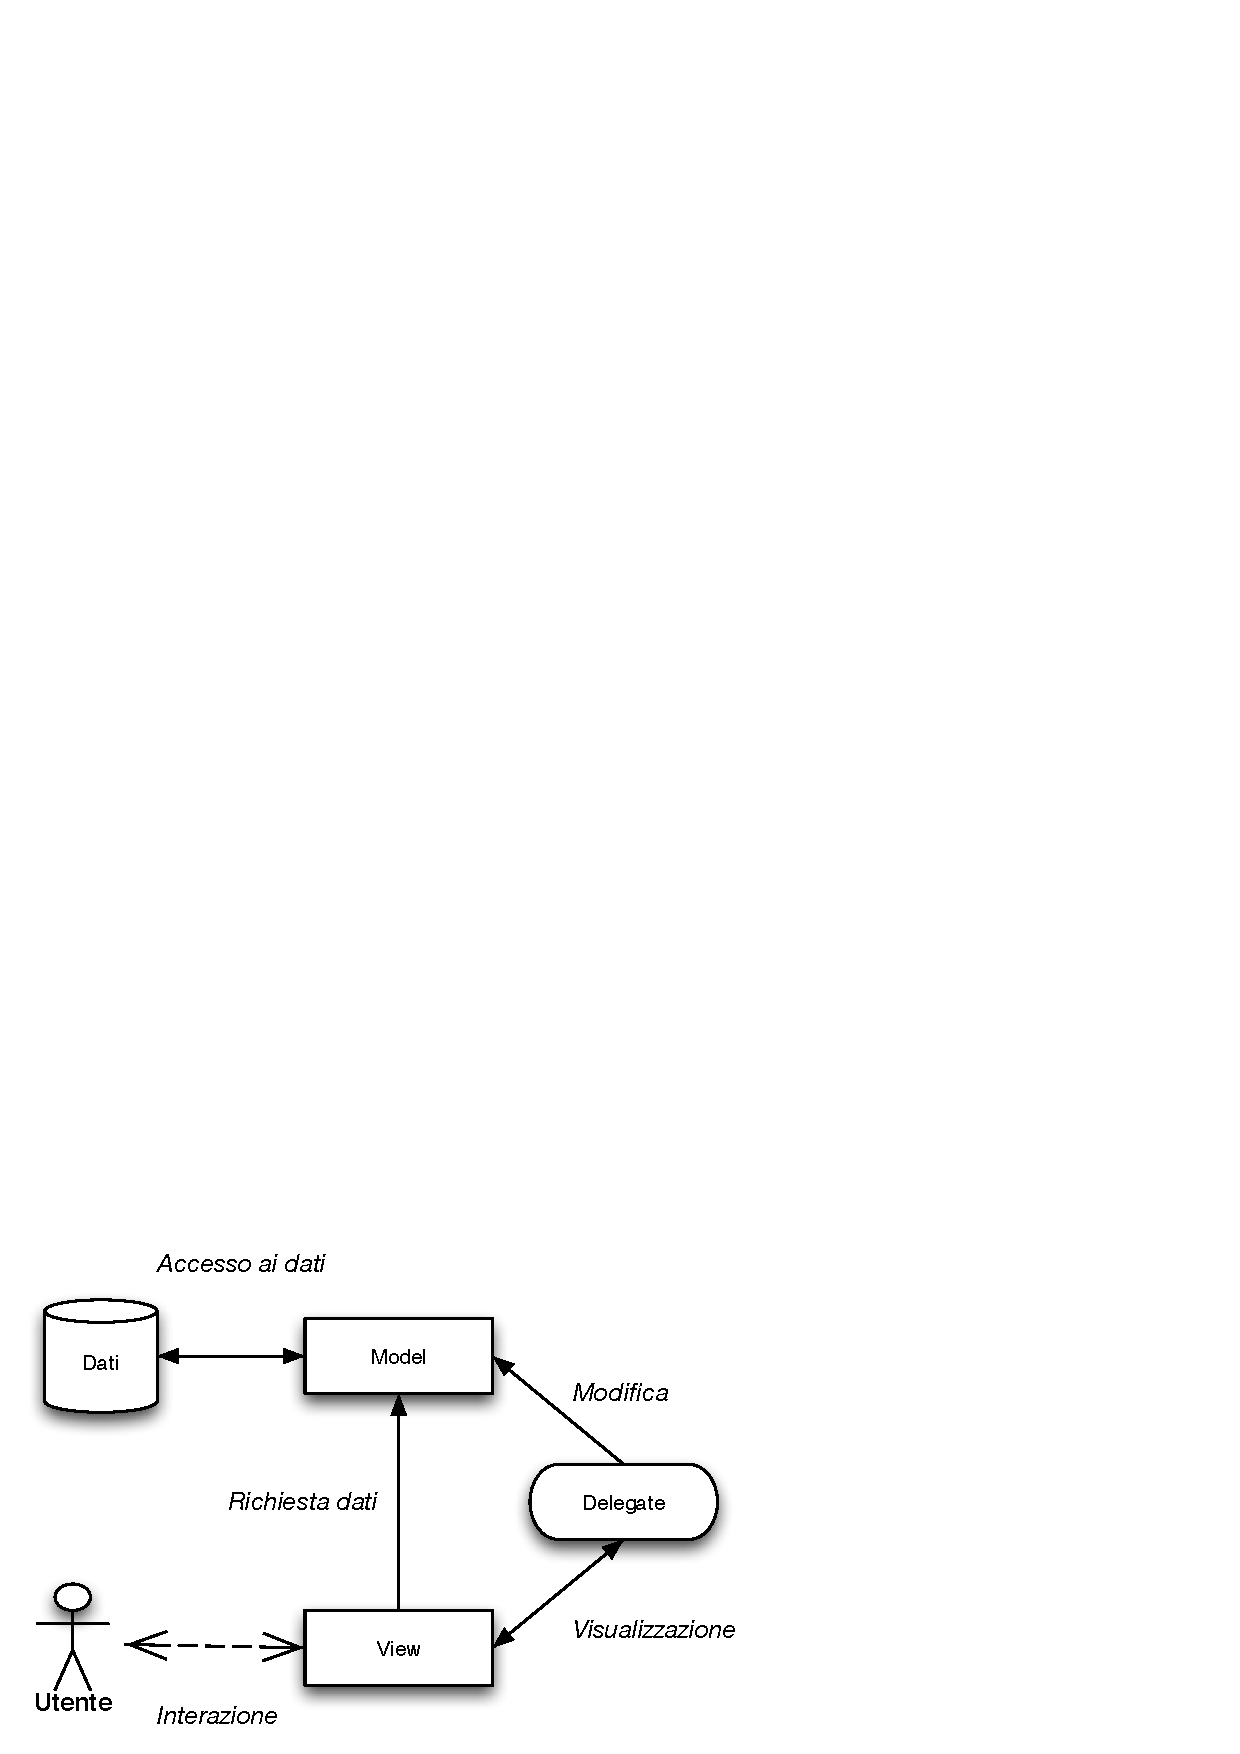
\includegraphics{images/mvd.png}
\caption{Diagramma delle interazioni nel pattern MVD in Qt}
\label{default}
\end{center}
\end{figure}


In quanto scritto fin'ora è possibile intravedere i benefici principali che derivano dall'utilizzo di questa architettura. 

In primo luogo, è possibile presentare all'utente i dati in maniera diversa senza per questo doverli duplicare o reimplementare i metodi di accesso ad essi. Per far ciò sarà sufficiente realizzare più view differenti, lasciando inalterato il model. Viceversa, se viene a cambiare il modo in cui i dati sono memorizzati, ad esempio passando dall'uso di un semplice file di testo all'uso di un databae, non sarà necessario apportare modifiche al view, poiché questa entità è per costruzione agnostica rispetto alla strategia di accesso ai dati.

Questa architettura libera inoltre il programmatore dal compito oneroso di dover sincronizzare manualmente i dati mostrati nell'interfaccia con i dati effettivamente memorizzati, specialmente in seguito ad un'interazione dell'utente con l'interfaccia. Siccome è la view che si occupa di richiedere i dati al model nel caso in cui venga richiesta una modifica nella visualizzazione, basterà aggiornare i dati in un solo punto e la modifica verrà propagata in maniera automatica anche a tutte le view che devono mostrare tali informazioni. 

Sussiste anche un vantaggio in termini prestazionali: siccome le view hanno consapevolezza dei dati esatti che è necessario mostrare, si limitano a richiedere quelli strettamente indispensabili in base alla visuale che l'utente ha sull'interfaccia in un determinato istante. Per fare un esempio, a fronte di qualche migliaia di record presenti nella base dati, è improbabile doverli mostrare tutti contemporaneamente all'utente in un'ipotetica tabella. Sarà la view che richiederà al model solamente il sottoinsieme di record da mostrare effettivamente quando l'utente provocherà l'evento corrispondente allo scorrimento verticale della tabella. Come risultato si ottiene una gestione più efficiente della memoria da parte dell'applicazione e un'interfaccia più reattiva.

%TODO: descrivere la possiiblità di creare in PyQt custom model e view. o di utilizzare le più comuni già presenti (treeview, etc)

\section{Il componente QtWebKit}

Come è stato detto in precedenza, si è scelto di utilizzare il framework Qt per sviluppare l'applicazione soprattuto per la possibilità di utilizzare al suo interno il motore di rendering WebKit, senza dover ricorrere a librerie esterne. Il componente QtWebKit è risultato essere ben integrato nel framework ed è stato possibile utilizzarne le potenzialità in maniera elegante ed efficace.

Siccome al centro delle funzionalità dello strumento da sviluppare si trova l'interazione con un'applicazione web, questo componente del framework ne ha costituito la parte principale, attorno a cui gli altri moduli si trovano a ruotare.

\subsection{WebKit rendering engine}

WebKit è un motore di rendering per visualizzare documenti che utilizzando i linguaggi di markup HTML ed SVG per definire il contenuto, CSS per regolarne gli stili di visualizzazione e Javascript come linguaggio di scripting per manipolare il Document Object Model (DOM). I due componenti principali al suo interno, realizzati in C++, sono il WebCore, responsabile per il rendering dei documenti sullo schermo, e il JavaScriptCore, che implementa all'interno di WebKit l'interprete Javascript. Nelle sue ultime versioni, l'interprete Javascript in WebKit compila questo linguaggio di scripting direttamente in codice macchina, migliorandone notevolmente i tempi di esecuzione.

Dopo che nel giugno 2005 Apple ha annunciato il rilascio di WebKit alla comunità open source con licenza LGPL e BSD, ne è stato effettuato il porting in svariati framework, tra qui Qt, sfruttando il fatto che WebKit, rispetto alle soluzioni alternative, si configura come un porgetto più snello e modulare, quindi più facilmente integrabile.

Oltre che alla possibilità di mostrare sullo schermo le pagine web di cui è necessario verificare il comportamento, il componente QtWebKit è stato fondamentale nello sviluppo dell'applicazione per definire ed eseguire materialmente i test. Di particolare interesse si è rivelata l'interazione instaurabile grazie a QtWebKit tra la parte di applicazione desktop in Python e la pagina web in esame. Grazie a questo motore di rendering è infatti stato possibile iniettare ed eseguire nel contesto della pagina web del codice Javascript generato dalla parte di applicazione in Python sotto forma di stringhe di testo, accedere e manipolare il DOM del documento tramite l'API di QtWebKit, ed infine far comunicare in maniera bidirezionale le due parti attraverso un sistema di conversione automatico da oggetti definiti in Python ad oggetti utilizzabili in Javascript all'interno della pagina web.

\subsection{Interazione tra QtWebKit ed il DOM}

Attraverso le classi QWebElement e QWebElementCollection il framework Qt permette al programmatore di manipolare il DOM della pagina web correntemente caricata da QtWebKit. Nello specifico, QWebElement rappresenta un singolo nodo dell'albero del documento, e mette a disposizione i metodi per modificarne gli attributi o il contenuto, per accedere ai nodi discendenti o al nodo padre visitando l'albero DOM e per appendere ad esso nuovi elementi come suoi discendenti diretti.

I nodi del DOM sono poi selezionabili specificando un selettore CSS. E' poi possibile richiamare un metodo Javascript su di un oggetto di tipo QWebElement, sistema utile ad esempio per simulare un evento nel DOM.

\subsection{QtWebKit Bridge}

Oltre ai metodi appena descritti, esiste un altro meccanismo all'interno del framework Qt per far comunicare l'applicazione in Python con una pagina web, Questo meccanismo, definito con il nome QWebKit  Bridge, estende l'interprete Javascript di WebKit consentendogli di lavorare con oggetti di classe QObject, definiti all'interno del framework. 

Questa classe, che costituisce il cuore delle funzionalità di Qt, oltre a realizzare il meccanismo di eventi basato su signal e slot consente di definire proprietà per le sue istanze in maniera dinamica, ossia durante l'esecuzione del programma. Questa capacità di introspezione viene sfruttata per poter passare dinamicamente da un oggetto QObject ad un oggetto Javascript e viceversa, data l'analogia che sussiste tra le proprietà dinamiche di entrambi. Naturalmente, il framework si occupa in maniera trasparente di convertire i tipi di dato da un ambiente all'altro: Qt gestisce ad esempio la conversione sia di tipi semplici, come dal tipo QString, definito nel framework, al tipo string in Javascript, sia di oggetti più complessi, come liste di tipo QList in array Javascript.

Particolarmente interessante è poi la possibilità di selezionare un nodo del DOM in uno script tramite l'API Javascript per poi passarlo al contesto Python, dove esso potrà essere manipolato sotto forma di oggetto di tipo QWebElement. 

Allo stesso modo, anche il meccanismo di slot e signal funziona in maniera trasparente tra il contesto Python e quello Javascript, a patto che il signal venga definito nel contesto dell'applicazione. Dall'ambiente Javascript è consentito ad esempio stabilire una connessione tra signal e slot di due oggetti messi a disposizione dall'esterno, oppure associare ad un signal emesso in Python uno slot rappresentato da una funzione definita in un oggetto Javascript. L'unico vincolo a questo sistema molto potente di condivisione è rappresentato dal fatto che, per motivi di sicurezza, l'applicazione deve indicare in maniera esplicita quali oggetti sono accessibili al contesto Javascript.

Come si può immaginare, le interazioni appena descritte aprono numerose possibilità interessanti al programmatore, consentendogli di implementare le funzionalità progettate nel contesto a cui più si addicono. Come evidenziato nella documentazione di Qt, il confine tra l'applicazione web e quella desktop diventa molto labile e ciò permette in molti casi di sfruttare le peculiarità migliori di questi due mondi. Si possono ad esempio realizzare applicazioni web che sono mantenute per comodità su di un server remoto, ed estenderne le funzionalità attraverso un'applicazione desktop che utilizza il componente QWebKit per superare le limitazioni tradizionalmente imposte da un browser, sia dal punto di vista prestazionale, sia da quello dell'interazione con il sistema operativo.

Nel nostro caso, questo interessante sistema è stato sfruttato per realizzare lo strumento di testing progettato. Uno dei vantaggi apportati, sicuramente da sottolineare, è stato riscontrato nel poter impiegare le migliori tecnologie disponibili in entrambi i contesti: per manipolare il DOM e per gestire gli eventi nell'ambiente web si è scelto di utilizzare la libreria jQuery, che offre un'interfaccia estremamente potente ed elegante per questi scopi, senza doverne riscrivere da zero le funzionalità  necessarie all'interno dell'applicazione. jQuery consente di gestire il DOM e gli eventi in modo molto più efficace ad esempio rispetto al componente QWebKit, perciò si è scelto di iniettare questa la logica sotto forma di codice Javascript nelle pagine web sotto esame, senza doversi preoccupare dell'interazione con la parte di codice in Python. Uno dei risultati più soddisfacenti durante lo sviluppo dello strumento per il testing è stato proprio l'alto livello di integrazione tra le tecnologie migliori a disposizione per ciascuna funzionalità da implementare.

%TODO: inserire codice?

\section{jQuery}

JQuery è una libreria in Javascript per facilitare ed uniformare tra i diversi browser la manipolazione del DOM, la gestione degli eventi, le animazioni e l'uso di richieste asincrone (AJAX). Rilasciata con doppia licenza MIT e GPL nel 2006, risulta essere ad oggi la libreria Javascript più utilizzata nel web [http://trends.builtwith.com/javascript/JQuery]. 

Il suo uso così diffuso è dovuto, oltre che alle prestazioni in linea con altre librerie analoghe, soprattutto all'interfaccia API semplice ed intuitiva, che permette di concentrarsi sulle funzionalità da sviluppare piuttosto che sui dettagli di basso livello. Sotto questo aspetto, jQuery si avvantaggia grazie all'implementazione di un'API di tipo \emph{fluent}, in cui è possibile concatenare di seguito più chiamate ai metodi di un oggetto, grazie al fatto che i metodi, dopo aver eseguito la manipolazione sull'oggetto, restituiscono ancora un'istanza della classe di partenza. Per rendere l'idea della leggibilità del codice scritto in jQuery, di seguito viene riportato un esempio:

\lstinputlisting[caption=Esempio di utilizzo della libreria jQuery ]{code/jquery_ex_1.js}

Attraverso queste poche istruzioni vengono prima selezionati i nodi del DOM di tipo DIV con classe "test", poi si accede ai rispettivi nodi figli di tipo A, che non siano però i primi nell'ordine. Di questi viene infine modificato l'attributo href ed assegnata una funzione di callback per l'evento click. 

Uno dei moduli più interessanti della libreria jQuery è proprio il sistema di selezione e di manipolazione del DOM. Nell'ambito dell'applicazione sviluppata, si è scelto di utilizzare proprio queste funzionalità di alto livello messe a disposizione dalla libreria poiché non si è riscontrato lo stesso livello di flessibilità in altre librerie sviluppate in Python.

Come visto nel capitolo relativo agli obiettivi dello strumento, due delle caratteristiche fondamentali che si è deciso di ottenere consistono nella semplicità di utilizzo e in un certo grado di robustezza dei test definiti. La scelta del sistema di selezione dei nodi del DOM nel contesto della pagina sotto esame gioca un ruolo fondamentale per il raggiungimento di entrambi questi requisiti. Molte delle soluzioni esistenti che sono state analizzate in fase preliminare utilizzano principalmente selettori XPath, che presentano però alcuni svantaggi rispetto ai selettori CSS. Si è deciso quindi di utilizzare i selettori CSS e si sono analizzate varie librerie che consentissero di accedere ai nodi del DOM mediante selettori CSS, valutando però anche la differente capacità espressiva rispetto all'XPath.

Inizialmente si è provato ad utilizzare la libreria pyquery [http://pypi.python.org/pypi/pyquery], scritta in Python, che sulla carta sembrava fornire un buon sistema di manipolazione del DOM, ispirandosi decisamente all'API di jQuery. Dopo alcuni esperimenti di utilizzo più approfondito ci si è però scontrati con alcuni bug e caratteristiche mancanti, necessarie per supportare l'algoritmo di generazione automatica dei selettori per i test sull'interfaccia della pagina web. 

Piuttosto che procedere con la correzione dei bug e l'implementazione delle caratteristiche mancanti, è sembrato più produttivo utilizzare direttamente la libreria jQuery per accedere al DOM della pagina web oggetto dei test e per implementare l'algoritmo di generazione dei selettori, sfruttando poi tecnologia QWebKit Bridge per comunicare in maniera trasparente con la parte applicativa scritta in Python.

\subsection{Un confronto tra i selettori CSS ed XPath}

Come è stato scritto in precedenza, uno dei vincoli progettuali stabiliti durante la fase di analisi dello strumento da sviluppare è stato l'utilizzo di selettori CSS piuttosto che selettori XPath per identificare gli elementi del DOM sui quali simulare gli eventi e stabilire delle assertion. Verrà presentato ora un confronto tra queste due tipologie di selettori, cercando di evidenziare gli aspetti che hanno influenzato la scelta compiuta. Per le osservazioni principali ci si è basati sugli spunti offerti in occasione della conferenza "Selenium meetup", tenutasi l'11 Maggio 2011 presso i Mozilla Office in California, durante la quale si è tenuto un intervento su questo tema.

Prima di confrontare alcune caratteristiche di questi due meccanismi di selezione, è opportuno chiarire la loro differente natura per comprenderne meglio le limitazioni ed i vantaggi intrinseci.

XPath, abbreviazione di XML Path Language, è un linguaggio per la selezione dei nodi all'interno di un documento XML. La versione 1.0, standardizzata dal W3C nel 1999, nacque appunto con l'obiettivo ben specifico di fornire una sintassi per individuare un elemento nell'albero XML attraverso l'uso di un percorso simile a quello utilizzato nel formato degli URL o di un filesystem, nei quali il carattere \\ è utilizzato per separare i livelli gerarchici. Attraverso XPath è possibile selezionare i nodi sia rispetto ad un percorso assoluto nell'albero, sia ad uno relativo ad un altro elemento specificato. XPath è in grado inoltre di specificare percorsi sia in senso ascendente che discendente nella gerarchia rappresentata dalla struttura al albero. Il linguaggio XPath è inoltre arricchito da un corposo insieme di funzioni, che operano su stringhe, numeri e valori booleani. Esse forniscono maggiore capacità espressiva, ad esempio permettendo di selezionare elementi in base al loro contenuto, al formato della stringa contenuta in un determinato attributo, oppure di filtrare i risultati ottenuti combinando predicati di tipo logico su insiemi di nodi selezionati.

Il linguaggio CSS (Cascading Style Sheets) è invece nato per tutt'altre finalità. Esso è infatti è costituito da una serie di regole per definire l'aspetto grafico e la formattazione di un documento scritto utilizzando l'XML o i suoi formati derivati, principalmente l'HTML. Il primo standard, sviluppato dal W3C, è stato rilasciato nel 1996. Per applicare le regole di stile definite ad un certo insieme di nodi del documento, la specifica CSS definisce un sistema di selezione, che con il passare degli anni si è arricchito notevolmente di nuove caratteristiche fino all'attuale versione 3, rimanendo comunque più semplice rispetto ad XPath. 

La semplicità dei selettori CSS implica però una minore potenza rispetto ai selettori XPath. Tra le limitazioni principali, non è possibile risalire nell'albero utilizzando un selettore CSS, ma solo specificare regole di selezione in maniera discendente, ossia da un nodo padre verso i nodi figli. Questa limitazione deriva soprattutto dal fatto che l'obiettivo principale della specifica CSS non è la selezione dei nodi e si è preferito limitarne le funzionalità a quelle di uso più comune per la presentazione dei documenti e per agevolarne un'implementazione il più omogenea possibile da parte dei vari browser. La specifica CSS definisce poi un insieme di pseudo-elementi utilizzabili nei selettori, i quali implementano però solamente un sottoinsieme delle funzionalità esprimibili tramite le funzioni di XPath.

Sebbene quindi i selettori CSS siano effettivamente meno potenti rispetto al tipo XPath, alcuni fattori ne hanno determinato la maggiore diffusione di utilizzo che è riscontrabile oggi, specialmente nell'ambito legato alle applicazioni web.
Tra questi fattori va incluso sicuramente il progressivo abbandono del formato XML in favore di quello JSON che si è verificato negli ultimi anni. Quest'ultimo formato di codifica, essendo di fatto più maneggevole e meno verboso rispetto all'XML, ha trovato infatti largo impiego in ambito web e molti linguaggi dinamici, come Python, PHP o Ruby integrano librerie standard che forniscono un maggiore supporto all'uso questo formato. 

\begin{figure}[htbp]
\begin{center}
\includegraphics[width=\textwidth]{images/byexml.png}
\caption{Statistica sul declino dell'uso di API in XML, http://blog.programmableweb.com/2011/05/25/1-in-5-apis-say-bye-xml/}
\label{default}
\end{center}
\end{figure}

Per citare alcuni dati pratici, sia Facebook che Twitter, nelle utlime versioni della loro API pubblica, hanno scelto di deprecare l'utilizzo dell'XML come sistema per convogliare le risposte alle richieste dei client e attualmente supportano esclusivamente il formato JSON. [https://dev.twitter.com/blog/changing-trends-api, http://developers.facebook.com/docs/reference/api/].

Ciò ha certamente portato ad un minore interesse da parte degli sviluppatori verso il linguaggio XPath, nato per essere usato in accoppiata con il formato XML. Oltretutto, i selettori CSS, benché meno potenti, sono sufficienti per gestire in maniera più semplice la grande maggioranza delle situazioni di interesse pratico.  

\subsubsection{Leggibilità}

Per rendersi conto della differente leggibilità tra selettori XPath e CSS, in favore di questi ultimi, è sufficiente osservare la tabella seguente, che mette a confronto i due tipi di selettori per lo stesso scopo: 

\begin{table}[htdp]
\caption{comparing selectors}
\begin{center}
\begin{tabular}{|c|c|c|}
\hline
\verb|div#foo| & \verb|div[@id="foo"]| & Seleziona l'elemento DIV con id "foo" \\\hline
\verb|div.foo| & \verb|//div[contains(concat(' ',normalize-space(@class),' '),' foo')]| & Seleziona l'elemento DIV che ha una classe "foo" \\\hline
\verb|p:first-child| & \verb|*[1]/self::p| & Seleziona l'elemento P che è il primo figlio del suo elemento padre \\\hline
\verb|p + a| & \verb|p/following-sibling::*[1]/self::a| & Seleziona gli elementi A preceduti immediatamente da un elemento P \\\hline
\verb|table#foo tr.test td:nth(2)| & \verb|//table[@id="foo"]//tr[@class="test"]//td[2]| & Seleziona l'elemento TD contenuto nella gerarchia specificata \\\hline

\end{tabular}
\end{center}
\label{comparing xpath vs css}
\end{table}

Come si può osservare, i selettori CSS risultano essere nella media più semplici e di più immediata comprensione. Queste caratteristiche fanno quindi sì che i test definiti tramite selettori CSS risultino maggiormente mantenibili nel lungo periodo.

\subsubsection{Prestazioni}

%TODO: è il caso di aggiungere?

\subsubsection{Utilizzo con jQuery}

Dalla versione 1.3, la libreria jQuery ha scelto di non supportare più i selettori di tipo XPath nella sua API. L'uso di selettori CSS è quindi una scelta obbligata se si decide di impiegare jQuery senza dipendere da plugin esterni. 

\chapter{Architettura dello strumento di testing}

In questo capitolo viene descritta l'architettura ...

\section{Modulo main.pyw}

Questo modulo costituisce il punto di ingresso dell'applicazione. La classe MainWindow rappresenta la finestra principale, ed eredita le caratteristiche della classe QMainWindow, definita nel framework PyQt. A differenza delle normali finestre di dialogo, la finestra principale deve essere unica all'interno dell'applicazione e prevede l'eventuale spazio per un barra dei menù, una barra di stato, un'area centrale in cui verranno posizionati i widget dell'interfaccia ed infine una serie di dock window, ossia finestre posizionabili e ridimensionabili dall'utente contenute nella finestra principale.

\begin{figure}[htbp]
\begin{center}
\includegraphics{images/mainwindowlayout.png}
\caption{Zone principali di una MainWindow}
\label{default}
\end{center}
\end{figure}

Nel costruttore della classe MainWindow sono inizializzate le strutture dati principali usate internamente per mantenere in memoria lo stato dell'applicazione e sono posizionati i componenti visuali. Si è cercato di mantenere la logica vera e propria dell'applicazione in moduli e classi esterni, per facilitare la gestione del codice. Di conseguenza gli unici due compiti delegati alla classe principale riguardano la costruzione dell'interfaccia grafica e il collegamento tra i segnali emessi dai widget in seguito all'interazione dell'utente e le funzioni di callback per la gestione degli eventi.

\subsection{Costruzione dell'interfaccia grafica}

Per la costruzione dell'interfaccia grafica esistono due metodologie possibili nell'ambito del framework Qt. La prima soluzione prevede la costruzione ed il posizionamento programmatico dei widget e dei layout, definendo cioè il modo in cui l'interfaccia sarà composta tramite chiamate nel codice agli appositi metodi delle classi che incapsulano i componenti visuali.

La seconda alternativa contempla invece l'uso di uno strumento visuale per questo compito, chiamato QtDesigner [http://doc.trolltech.com/4.7/designer-manual.html]. Utilizzando questo editor il programmatore può disegnare visivamente l'interfaccia grafica trascinando i widget da una barra direttamente sulla finestra principale e posizionarli a piacimento senza ricorrere al codice. E' inoltre possibile gestire visivamente anche le connessioni tra signal e slot dei widget in maniera rapida tramite un apposito editor. 

Le informazioni fornite a QtDesigner sono memorizzate successivamente in un file con estensione .ui, che deve essere poi tradotto in codice Python tramite un'apposita utility eseguibile da linea di comando, prima di poter essere utilizzato.

Sebbene l'uso di questo strumento possa risultare decisamente produttivo, specialmente per creare prototipi o per gestire più efficacemente interfacce grafiche complesse, si è scelto di non utilizzarlo e di costruire l'interfaccia dell'applicazione in maniera programmatica. La scelta è stata fatta soprattutto per motivi didattici, in quanto l'utilizzo di questo strumento visuale avrebbe potenzialmente nascosto la filosofia con la quale il framework Qt gestisce il posizionamento dei widget, ostacolando l'apprendimento e rendendo poi più difficili interventi manuali di modifica in un secondo momento. Inoltre, la costruzione programmatica fornisce sicuramente un grado di controllo maggiore per un'interfaccia non estremamente complicata come quella per l'applicazione da realizzare.

Il widget principale dell'interfaccia, che raggruppa al suo interno la maggioranza degli altri componenti, è un widget di tipo QSplitter. Esso permette di posizionare al suo interno altri widget all'interno di due aree separate da una barra, ridimensionabili in larghezza o in altezza dall'utente. In questo caso, si è impostato l'orientamento in senso orizzontale, in modo da ospitare nella zona sinistra il componente del browser e nella zona destra l'elenco delle azioni e delle asserzioni registrate. In base alla risoluzione dello schermo, l'utente può ridimensionare lo spazio assegnato in orizzontale ad una delle due aree nel caso avesse la necessità di visualizzare più o meno informazioni sulla registrazione attuale.

Una volta istanziato il widget QSplitter ed averne assegnato una referenza ad una proprietà della classe, esso è stato impostato come widget centrale della finestra tramite il metodo QWindow::setCentralWidget. 

\lstinputlisting[caption=Definizione e posizionamento del widget principale ]{code/ui/main_splitter.py}

Di seguito sono creati e posizionati nelle due aree i widget delle tre aree principali, ossia la barra dell'indirizzo, il browser e la lista delle azioni registrate. Il codice per questo scopo è stato suddiviso in altrettanti metodi protetti della classe MainWindow, per una migliore leggibilità e mantenibilità. 

\subsubsection{La barra degli indirizzi}

Per realizzare la barra dell'indirizzo, attraverso la quale caricare una pagina nel browser sottostante, sono stati utilizzati un campo di testo semplice QLineEdit e un bottone a pressione di tipo QPushButton. Questi ultimi sono stati posizionati in orizzontale tramite un layout di tipo QHBoxLayout, che gestisce in maniera automatica il posizionamento fluido del suo contenuto in base alle dimensioni del contenitore.

All'interno del metodo chiamato alla pressione del pulsante, è stato inserita della semplice logica per rendere compatibile il formato dell'url inserito dall'utente con quello atteso dal componente del browser. Poiché quest'ultimo internamente si aspetta un URL completo di protocollo, esso viene aggiunto in maniera automatica se non viene digitato nel campo di testo dall'utente, come avviene nei normali browser.

Siccome la visita di un determinato indirizzo viene considerata come un evento interessante ai fini della simulazione, se la funzione di registrazione è attiva questa azione viene aggiunta all'elenco di quelle compiute dall'utente. Usando questa caratteristica è possibile definire allo stesso modo il punto di partenza di un test: basterà infatti attivare la registrazione, inserire l'indirizzo da visitare e da lì cominciare con l'interazione.

\subsubsection{Il browser}

Il widget di tipo QWebView, che visualizza effettivamente il contenuto delle pagine web, non viene istanziato e gestito direttamente dal modulo principale, come avviene per tutti gli altri widget. Si è infatti scelto di incapsularne le funzionalità all'interno del modulo simulator, descritto in seguito nel dettaglio. Tutta la parte relativa alla simulazione e all'interazione con l'applicazione web viene implementata attraverso i metodi della classe QWebPage e QWebView, pertanto dall'esterno il modulo simulator viene visto come un oggetto opaco. 

Come si è visto però il posizionamento dei widget nell'interfaccia è responsabilità esclusivamente della classe MainWindow. Per questo motivo, da essa è possibile ottenere un riferimento al componente del browser attraverso il metodo simulator::getWidget(). Una volta fatto ciò, il widget di classe QWebView.

Al di sotto del browser sono state posizionate una label per mostrare lo stato di caricamento delle pagine da visualizzare ed una per mostrare all'utente il selettore CSS selezionato tramite l'apposito strumento. Queste informazioni sono gestire dal modulo simulator, e per poterle reperire dall'esterno si è sfruttato il sistema di gestione degli eventi offerto da Qt. Grazie ad esso, la classe Simulator definisce ed emette svariati segnali personalizzati, ai quali sono connessi gli slot definiti nella classe MainWindow. Quest'ultima viene quindi notificata quando il simulatore esegue azioni di interesse per l'interfaccia grafica.

\lstinputlisting[caption=Comunicazione ad eventi tra MainWindow e Simulator ]{code/ui/loading_label.py}

Nel codice mostrato vengono connessi i segnali emessi dalla classe Simulator con i metodi di callback della classe MainWindow. In particolare, in corrispondenza dell'evento di inizio caricamento di una pagina, viene mostrata nell'interfaccia la label che notifica all'utente questo stato di attesa, poiché questa operazione può richiedere un certo periodo di tempo, a seconda della velocità di connessione.  

Sempre in questo estratto di codice, si può osservare la sintassi per ricevere segnali con parametri. In questo caso, il simulatore aggiunge all'evento di selezione di un elemento un parametro di tipo PyQt\_PyObject, contenente un'instanza della classe PickedData che incapsula le informazioni sulla selezione dell'utente. Questa particolare sintassi per il tipo del parametro da ricevere è dovuta alla conversione necessaria tra i tipi del framework Qt, definiti in C++, e i tipi del framework PyQt, definiti in Python. 

\subsubsection{La lista delle azioni}

La lista delle azioni è stata collocata nel pannello destro del widget QSplitter principale. Per realizzarla, si è scelto di utilizzare il componente QTreeView, il quale visualizza i dati tenendo conto di una gerarchia ad albero tra gli elementi da mostrare. I livelli intermedi possono essere contratti ed espansi, in modo che l'utente possa scegliere di quali informazioni mostrare i dettagli. 

Se la modalità di registrazione è attiva, in questo spazio vengono mostrate le azioni compiute dall'utente all'interno della pagina web che sono significative ai fini della simulazione, come il click sui link, la compilazione di campi testuali, eccetera. In aggiunta, tra un'azione e l'altra è possibile inserire le assertion, ossia particolari condizioni che il simulatore deve verificare durante l'esecuzione del test. Quest'ultime sono di fatto equiparabili in un certo senso alle azioni compiute dall'utente, in quando automatizzano i controlli visivi che dovrebbero essere effettuati per accertarsi del corretto funzionamento. Per questo motivo, sono presentate nella stessa porzione di interfaccia delle azioni, nell'ordine cronologico in cui sono state definite.

Per implementare la vista ad albero si è ricorsi al pattern MVC proposto dal framework PyQt, pertanto è stato necessario definire una classe model apposita che funge da tramite tra la struttura dati interna, nella quale le azioni registrate sono memorizzate, e la view, che deve mostrare tali dati secondo certi criteri nell'interfaccia. Questa implementazione verrà descritta più nel dettaglio in seguito, all'interno del paragrafo dedicato al modulo actions.

\lstinputlisting[caption=Costruzione della vista ad albero e connessione dei segnali ]{code/ui/action_tree.py}

Come si può osservare, attraverso il metodo setModel della classe QTreeView viene indicato al framework quale classe si intende adoperare come model per la vista istanziata.

Nelle righe successive vengono poi creati due pulsanti di tipo QToolButton e collegati i relativi eventi di click con i metodi che comunicano al simulatore di inziare la riproduzione delle azioni correntemente memorizzate, oppure di cancellare le azioni evidenziate.

Per quest'ultimo scopo nel metodo \verb|_onRemoveActionClicked| è necessario accedere direttamente al model impostato per la vista ad albero, poiché è questa classe che si occupa di gestire i dati, secondo il pattern MVC. Le azioni non vengono infatti rimosse direttamente richiamando un metodo della classe QTreeView. Sarà invece il model che notificherà la view di un cambiamento avvenuto nei dati sottostanti e ciò provocherà un'aggiornamento delle informazioni mostrate nell'interfaccia. In questo modo è garantita la sincronia dei dati in memoria con quelli presentati a video, senza che l'applicazione possa trovarsi in uno stato inconsistente sotto questo aspetto.

\subsubsection{La barra degli strumenti}

Creare una tipica barra degli strumenti è relativamente semplice all'interno del framework Qt: è sufficiente infatti richiamare il metodo addToolBar della classe QMainWindow, che come visto prevede già lo spazio per ospitarla. I vari pulsanti nella barra sono invece rappresentati da oggetti di tipo QAction, ai quali viene assegnata un'icona. 

Gli oggetti QAction non sono semplici pulsanti, ma rappresentano le azioni principali eseguibili dall'applicazione. Tramite appositi metodi si definiscono vari attributi di queste azioni, tra cui ad esempio le combinazioni di tasti che le attivano. La classe QAction viene definita in Qt per uniformare e centralizzare la gestione di queste azioni, che normalmente è possibile compiere in maniere differenti. Spesso infatti azioni come l'apertura o il salvataggio di un file sono raggiungibili sia dalla barra degli strumenti, sia dal menù principale dell'applicazione. Siccome l'azione che l'utente si aspetta di eseguire è in effetti la stessa, è opportuno che dal lato del codice venga utilizzata la stessa entità, in modo da evitare una possibile duplicazione.

I file di immagine per le icone utilizzate nell'applicazione sono gestiti tramite un file esterno in formato XML, nel quale indicare le risorse impiegate con i percorsi ed i nomi dei file. Per ogni risorsa è anche possibile specificare un identificativo utilizzabile nell'applicazione per reperire il file in maniera più agevole e leggibile, senza specificarne il percorso fisico. Per poter usare questa lista di risorse, è necessario compilare il file XML in codice Python tramite l'utility \verb|pyrcc4| ed poi importarlo nell'applicazione come fosse un comune modulo in Python.

Siccome la creazione di un oggetto \verb|QAction| è un'operazione comune e richiede un discreto numero di linee di codice per assegnare l'icona, il testo di descrizione e la combinazione di tasti, è stato creato un metodo statico apposta nella classe \verb|Gui| del package \verb|Utilities|.

\section{Modulo simulator}

Il modulo \verb|Simulator| costituisce il cuore dell'applicazione, poiché raggruppa le classi utilizzate per interagire con l'applicazione web da testare. La classe \verb|Simulator| al suo interno sfrutta la tecnologia QWebKit e ne pilota l'interfaccia per gli scopi della simulazione. Dall'esterno quindi non è necessario interagire direttamente con il browser, poiché la classe Simulator ne astrae ed estende le funzionalità, introducendo i concetti di azione dell'utente, di asserzione e di simulazione.

Il componente QWebKit presenta un'architettura altamente modulare, che permette di riutilizzare singolarmente le diverse parti che lo compongono, in maniera efficiente. Nello specifico, è la classe \verb|QWebPage| che gestisce il caricamento delle pagine, la cronologia degli indirizzi visitati, le strategie di memorizzazione dei cookies, ed altri aspetti di alto livello. Ogni QWebPage contiene come minimo un oggetto di tipo \verb|QWebFrame|, che modella invece un frame definito tramite i tag HTML \verb|<frame>| o \verb|<iframe>|. Attraverso un \verb|QWebFrame| si può poi accedere alla rappresentazione del DOM, selezionando e modificando i nodi presenti, modellati a loro volta dalla classe QWebElement. 

Grazie alla modularità delle due classi appena descritte, si può evitare l'overhead dovuto al rendering vero e proprio della pagina web se questo non è necessario ai fini dell'applicazione (ad esempio poiché è sufficiente accedere alle informazioni nel DOM). Per visualizzare sullo schermo la pagina web è infatti disponibile l'apposita classe \verb|QWebView|, che essendo discendente della classe |QWidget| viene trattata come un qualsiasi altro componente dell'interfaccia grafica.

\subsubsection{Iniezione di codice Javascript nelle pagine web}

Per i motivi descritti nel capitolo riguardante le tecnologie utilizzate, si è scelto di accedere al DOM della pagina e di intercettare gli eventi dovuti all'interazione con l'utente tramite la libreria jQuery. Tutto il codice realizzato in javascript deve quindi poter essere iniettato all'interno della pagina web che viene caricata dal simulatore prima di poterne utilizzare le funzionalità. 

La classe QWebFrame fornisce un metodo apposta per questo scopo, chiamato \verb|evaluateJavaScript|. Come indica il nome, esso accetta come parametro una stringa di testo contenente del codice javascript, che viene eseguito nel contesto del frame specficato. Il valore di ritorno del metodo corrisponde al valore restituito dall'esecuzione dell'ultima istruzione Javascript.

Nel caso dell'applicazione sviluppata, viene ipotizzato l'utilizzo del solo frame principale. Questo vincolo ha semplificato la fase di iniezione del codice nelle pagine web, senza però limitare nel complesso le funzionalità dello strumento. Inoltre oggi l'uso dei frame all'interno delle pagine web viene fortemente sconsigliato poiché ne danneggiano l'usabilità e l'accessiblità, tant'è che i tag relativi all'inserimento dei frame sono stati rimossi dalla nuova specifica per l'HTML5 [http://www.w3.org/TR/html5-diff/\#absent-elements]. 

All'interno del costruttore della classe Simulator vengono letti i file che contengono la libreria jQuery ed i componenti dell'applicazione sviluppati in Javascript, ossia il registratore degli eventi, il generatore dei selettori CSS e lo strumento per selezionare gli elementi della pagina web (\verb|Picker|). Il contenuto di questi file viene quindi iniettato in ogni pagina web nel momento in cui il componente \verb|QWebPage| segnala che il caricamento della pagina è completata tramite l'apposito  \verb|signal|. 

Prima di iniettare effettivamente il codice Javascript, esso viene manipolato per evitare potenziali conflitti con il codice Javascript che potrebbe essere già presente nella pagina corrente. Per evitare conflitti tra i nomi delle variabili jQuery definisce un metodo apposito chiamato \verb|noConflict| che consente di usare questa libreria insieme ad altre che utilizzano il nome di variabile \verb|$| come alias per l'oggetto principale (succede ad esempio nel caso del framework Mootools [http://mootools.net/]). 

All'interno della classe Simulator viene perciò definito un alias speciale per la variabile di jQuery \verb|$|, che viene sostituito a questo simbolo in maniera automatica prima di eseguire il codice Javascript nel contesto della pagina web. Questo passaggio è dimostrato nel seguente estratto di codice:

\lstinputlisting[caption=Caricamento della libreria jQuery con modalità no-conflict]{code/ui/jquery_no_conflict.py}

Un altro aspetto da tenere in considerazione per il corretto funzionamento del codice Javascript iniettato interessa le tempistiche con le quali esso si trova a dover interagire con il DOM della pagina. Se il codice si trova infatti ad accedere al DOM mentre la costruzione dell'albero da parte del browser non è ancora completata, potrebbero verificarsi comportamenti inattesi poiché gli ultimi elementi della pagina potrebbero non essere ancora effettivamente stati aggiunti alla rappresentazione in memoria del DOM. La manifestazione tipica di questo fenomeno consiste quindi nella mancata selezione di alcuni elementi, considerati inesistenti. 

Siccome l'istante in cui viene terminato il caricamento della pagina a livello di rete non coincide necessariamente con l'istante in cui la rappresentazione in memoria del DOM è stata completata, per superare questo potenziale problema non si può fare affidamento semplicemente sul segnale \verb|loadFinished| emesso dalla classe \verb|QWebPage|. Fortunatamente, il framework jQuery fornisce una semplice soluzione alla questione grazie al metodo  \verb|$.ready()|. La funzione anonima passata a questo metodo, contenente il codice da eseguire, viene infatti eseguita solamente quando il caricamento del DOM è stato completato.

Oltre che per caricare il codice delle librerie, questo metodo è stato utilizzato anche per realizzare la parte di simulazione vera e propria, che viene descritta più dettagliatamente in seguito, nel paragrafo dedicato al package \verb|actions|. Per ora è sufficiente dire che le azioni dell'utente che sono state registrate, come il click su di un link, vengono rieseguite facendo eseguire all'interprete Javascript il codice apposito, che riproduce l'evento come se fosse stato generato dall'utente.

\subsubsection{Comunicazione tra Python e Javascript}

Come si è visto in precedenza, il framework PyQt fornisce anche un modo più sofisticato per interagire con il contesto web dall'applicazione in Python, che permette di utilizzare oggetti in Python in maniera trasparente anche all'interno del codice Javascript.

\subsection{Sincronizzazione tra richieste HTTP e flusso di simulazione}

Uno dei problemi principali che ci si è trovati ad affrontare durante lo sviluppo dello strumento per il testing è costituito dalla necessità di sincronizzare il flusso di esecuzione delle azioni simulate con i tempi di caricamento delle pagine web da parte di QWebKit. 

Sebbene sia stato appena descritto il metodo per attendere il completamento della rappresentazione del DOM prima di eseguire codice Javascript, esso non risolve il problema di stabilire la tempistica corretta con la quale far eseguire le azioni registrate al simulatore. E' infatti la parte di applicazione in Python che si occupa di pilotare il simulatore, stabilendo il momento in cui esso deve eseguire una determinata azione. Tale operazione deve essere iniziata però solamente quando la classe \verb|QWebPage| ha terminato il caricamento della pagina, poiché in caso contrario il codice Javascript da iniettare per eseguire materialmente la simulazione degli eventi e delle asserzioni avrebbe un comportamento potenzialmente non prevedibile. 

Per garantire la sincronizzazione temporale dei vari passi della simulazione, la classe \verb|Simulator| implementa il metodo \verb|wait_load|, mostrato nell'estratto seguente:

\lstinputlisting[caption=Gestione della sincronia da parte del simulatore]{code/simulator/wait_load.py} 

Per sospendere l'esecuzione della simulazione fino al completo caricamento della pagina corrente viene utilizzato un ciclo nel quale si controlla periodicamente il valore assunto della proprietà \verb|_load_status|. Il ciclo viene interrotto quando il valore assunto indica il termine della fase di caricamento, oppure quando scade un timeout, onde evitare che il tempo di attesa sia indefinito qualora si verifichino problemi. 

Il valore della variabile di stato \verb|_load_status| viene modificato in maniera asincrona dallo slot associato al segnale \verb|loadFinished()|, emesso dal componente del browser. Una volta ricevuto l'evento, la variabile di stato viene impostata con valore nullo, per indicare che non è in corso il caricamento di alcuna pagina.

Nel caso in cui il metodo di attesa venga invocato senza che sia effettivamente in corso un caricamento, il ciclo non viene eseguito.

La soluzione adottata non ha presentato particolari problemi di prestazioni pur implementando di fatto una forma di "busy form of waiting", poiché i tempi di attesa sono generalmente molto brevi e sono comunque controllati da un timeout. Una soluzione più elegante da questo punto di vista potrebbe contemplare l'utilizzo della programmazione concorrente mediante thread, che aggiungerebbe però un ulteriore livello di complessità all'applicazione senza aggiungere nulla però agli scopi finali.

L'effetto collaterale indesiderato consiste però nel fatto che, utilizzando il ciclo di attesa, l'interfaccia dell'applicazione smette di essere reattiva all'interazione con l'utente. Per superare questo ostacolo, si è fatto uso del metodo \verb|QCoreApplication.processEvents|, con il quale si impone manualmente al processo di processare gli eventi in coda in arrivo dal sistema operativo sottostante. Normalmente il loop degli eventi, tipico di ogni applicazione dotata di interfaccia, viene gestito internamente dal framework Qt, ma in questo caso è stato indispensabile interagirci direttamente.

Il metodo \verb|wait_load| viene invocato automaticamente quando viene simulata un'azione di click su di un elemento. Se il click non provoca il caricamento di una pagina o una richiesta asincrona, l'applicazione non si pone in stato di attesa. In questo modo il fase di registrazione non è necessario preoccuparsi di questo dettaglio tecnico.

\subsection{Simulazione e richieste AJAX}

La questione riguardante la sincronizzazione risulta ancora più delicata se decide di tenere in considerazione anche le richieste AJAX che possono essere eseguite dall'applicazione web. In questo caso, prima di simulare le azioni e le asserzioni successive si è costretti ad individuare una strategia per stabilire con certezza quando le eventuali richieste AJAX sono terminate, per poter poi proseguire con il flusso della simulazione. 

La maggiore complessità di questo problema rispetto al precedente risiede nella natura asincrona delle richieste AJAX. A differenza di quanto avviene per quest'ultime, il caricamento di una nuova pagina è un evento prevedibile durante il corso della simulazione, ed è pertanto gestibile in maniera efficace grazie al segnale \verb|loadFinished| emesso dalla classe \verb|QWebPage|. 

Poiché oramai la tecnologia AJAX trova impiego nella maggioranza delle applicazioni web recenti, è sembrato opportuno che lo strumento sviluppato supportasse il test di applicazioni che fanno uso di richieste asincrone, ricordando che tra gli obiettivi posti giocano un ruolo importante la semplicità d'uso e che l'utilizzatore per ipotesi può non avere competenze sulle tecnologie web utilizzate. 

A tale proposito si consideri questo semplice scenario d'uso: l'utente clicca su di un link e dietro le quinte l'applicazione web invia una richiesta AJAX al server. Il server risponde con un messaggio, ed il contenuto del DIV sottostante al link viene aggiornato con il messaggio ricevuto, senza che la pagina venga ricaricata. A questo punto si desidera definire un test che verifichi il corretto funzionamento dell'applicazione web in base a questo scenario. 

Affinché il test sia realizzabile, è necessario che il simulatore attenda il completamento della richiesta AJAX prima di eseguire l'asserzione definita dall'utente sul contenuto del messaggio visualizzato dopo il click sul link. Se ciò non avvenisse, il test fallirebbe solamente a causa delle tempistiche con cui viene effettuato.

Sono da tenere poi presenti le seguenti condizioni aggiuntive. In primo luogo, non è possibile prevedere a priori il tempo impiegato per completare la richiesta asincrona, poiché esso dipende da fattori esterni non controllabili, come il tempo di risposta del server, la dimensione della risposta e la congestione della rete. In aggiunta, differenti richieste AJAX possono essere originate in parallelo dalla stessa pagina, siccome potenzialmente l'utente può continuare ad interagire con l'interfaccia dell'applicazione web mentre questa attende il completamento di una precedente richiesta asincrona.

\begin{figure}[htbp]
\begin{center}
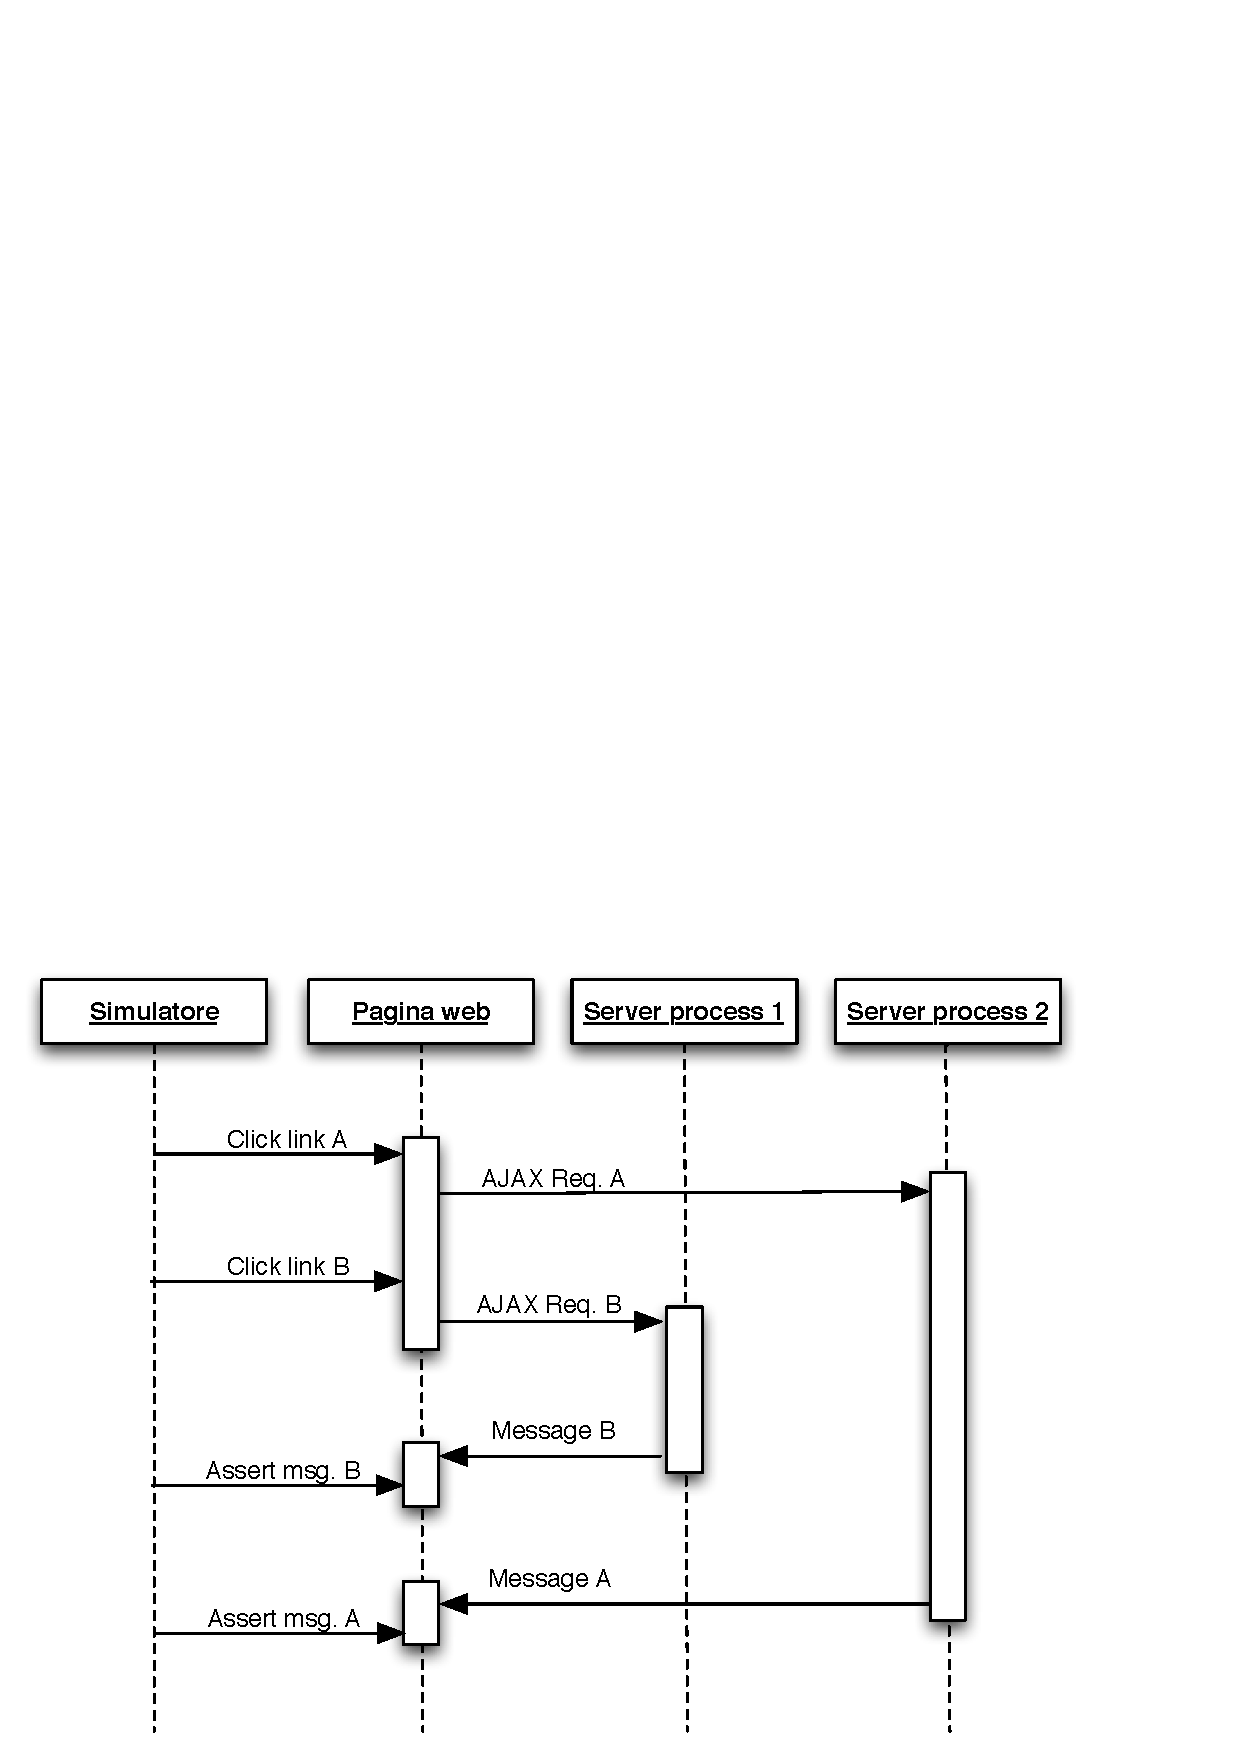
\includegraphics[width=\textwidth]{images/ajax_sync.png}
\caption{Sequence diagram per richieste AJAX parallele}
\label{fig:ajaxSequence}
\end{center}
\end{figure}

Nella figura ~\ref{fig:ajaxSequence} viene rappresentato un diagramma di sequenza che illustra la situazione descritta fino ad ora, con la corretta sequenza temporale in cui il simulatore deve effettuare le asserzioni nel caso in cui le richieste parallele ricevano risposte sfasate rispetto all'ordine di partenza.  

Per gestire le tempistiche in gioco per questo scenario non si può ricorrere al segnale utilizzato nel caso precedente, poiché questo non viene emesso dalla classe \verb|QWebPage| per le richieste asincrone generate una volta terminato il caricamento iniziale della pagina.

Per sapere quando una richiesta asincrona viene completata è stato necessario interagire ad un livello più basso del sistema, attraverso la classe \verb|QNetworkAccessManager|. Quest'ultima modella l'interazione a livello di rete del browser e permette di accedere anche ai dati delle singole richieste e risposte HTTP. Tra i segnali emessi, di particolare interesse è stato il segnale \verb|finished(QNetworkReply *)|, utilizzato per segnalare che è stata ricevuta una risposta ad una precedente richiesta e tale risposta viene passata come parametro al segnale. I dati di queste due entità sono incapsulati all'interno delle due classi \verb|QNetworkRequest| e \verb|QNetworkReply|.

Durante il caricamento della pagina il browser effettua diverse richieste HTTP attraverso il \verb|QNetworkAccessManager|, ad esempio per ricevere le immagini o altre risorse esterne alla pagina. Si è rivelato quindi necessario trovare un modo per distinguere le richieste AJAX dalle altre, che non richiedono un trattamento particolare. Per fare ciò si è scelto di analizzare gli header HTTP della richiesta, cercando come indicatori la presenza ed il valore del campo \verb|X-Requested-With|.

L'utilizzo di questo header particolare non è indicato nelle specifiche del W3C per quando riguarda le richieste di tipo XMLHttpRequest [http://www.w3.org/TR/XMLHttpRequest/], tuttavia può essere considerato uno standard de facto poiché tutti i maggiori framework Javascript (jQuery, MooTools, Prototype, YUI ed altri) lo includono automaticamente nelle richieste AJAX effettuate tramite queste librerie. Rimane però escluso il caso in cui l'applicazione sotto esame utilizzi il metodo nativo del browser per le richieste asincrone, senza aggiungere l'header \verb|X-Requested-With|. Sebbene sia probabilmente possibile stabilire un sistema di identificazione più raffinato, tenendo conto anche di questo caso, si è scelto di non approfondire la ricerca in questo senso per scarso interesse ai fini pratici, poiché oramai la stragrande maggioranza delle applicazioni web di una certa rilevanza si appoggiano su uno di questi framework Javascript [http://trends.builtwith.com/javascript].

\lstinputlisting[caption={Identificazione di una richiesta AJAX terminata}, label=code:ajax_sniffing]{code/simulator/ajax_sniffing.py}

Il procedimento appena descritto è mostrato nell'estratto ~\ref{code:ajax_sniffing}. Come si può osservare, dopo che una richiesta asincrona è stata completata viene aggiornato di conseguenza il valore della proprietà \verb|load_status|, campionato durante l'attesa dal simulatore all'interno del metodo \verb|wait_load|.

Nel caso di richiese AJAX in parallelo, siccome il simulatore ne attende in automatico il completamento, di fatto esse vengono eseguite in maniera serializzata durante la simulazione, anche se l'utente non ha atteso la risposta alla prima richiesta prima di effettuare la seconda. Questa serializzazione forzata risulta indispensabile per eseguire nell'ordine corretto le eventuali asserzioni definite durante il test, senza che il loro risultato dipenda da fattori esterni non riproducibili.

\begin{figure}[htbp]
\begin{center}
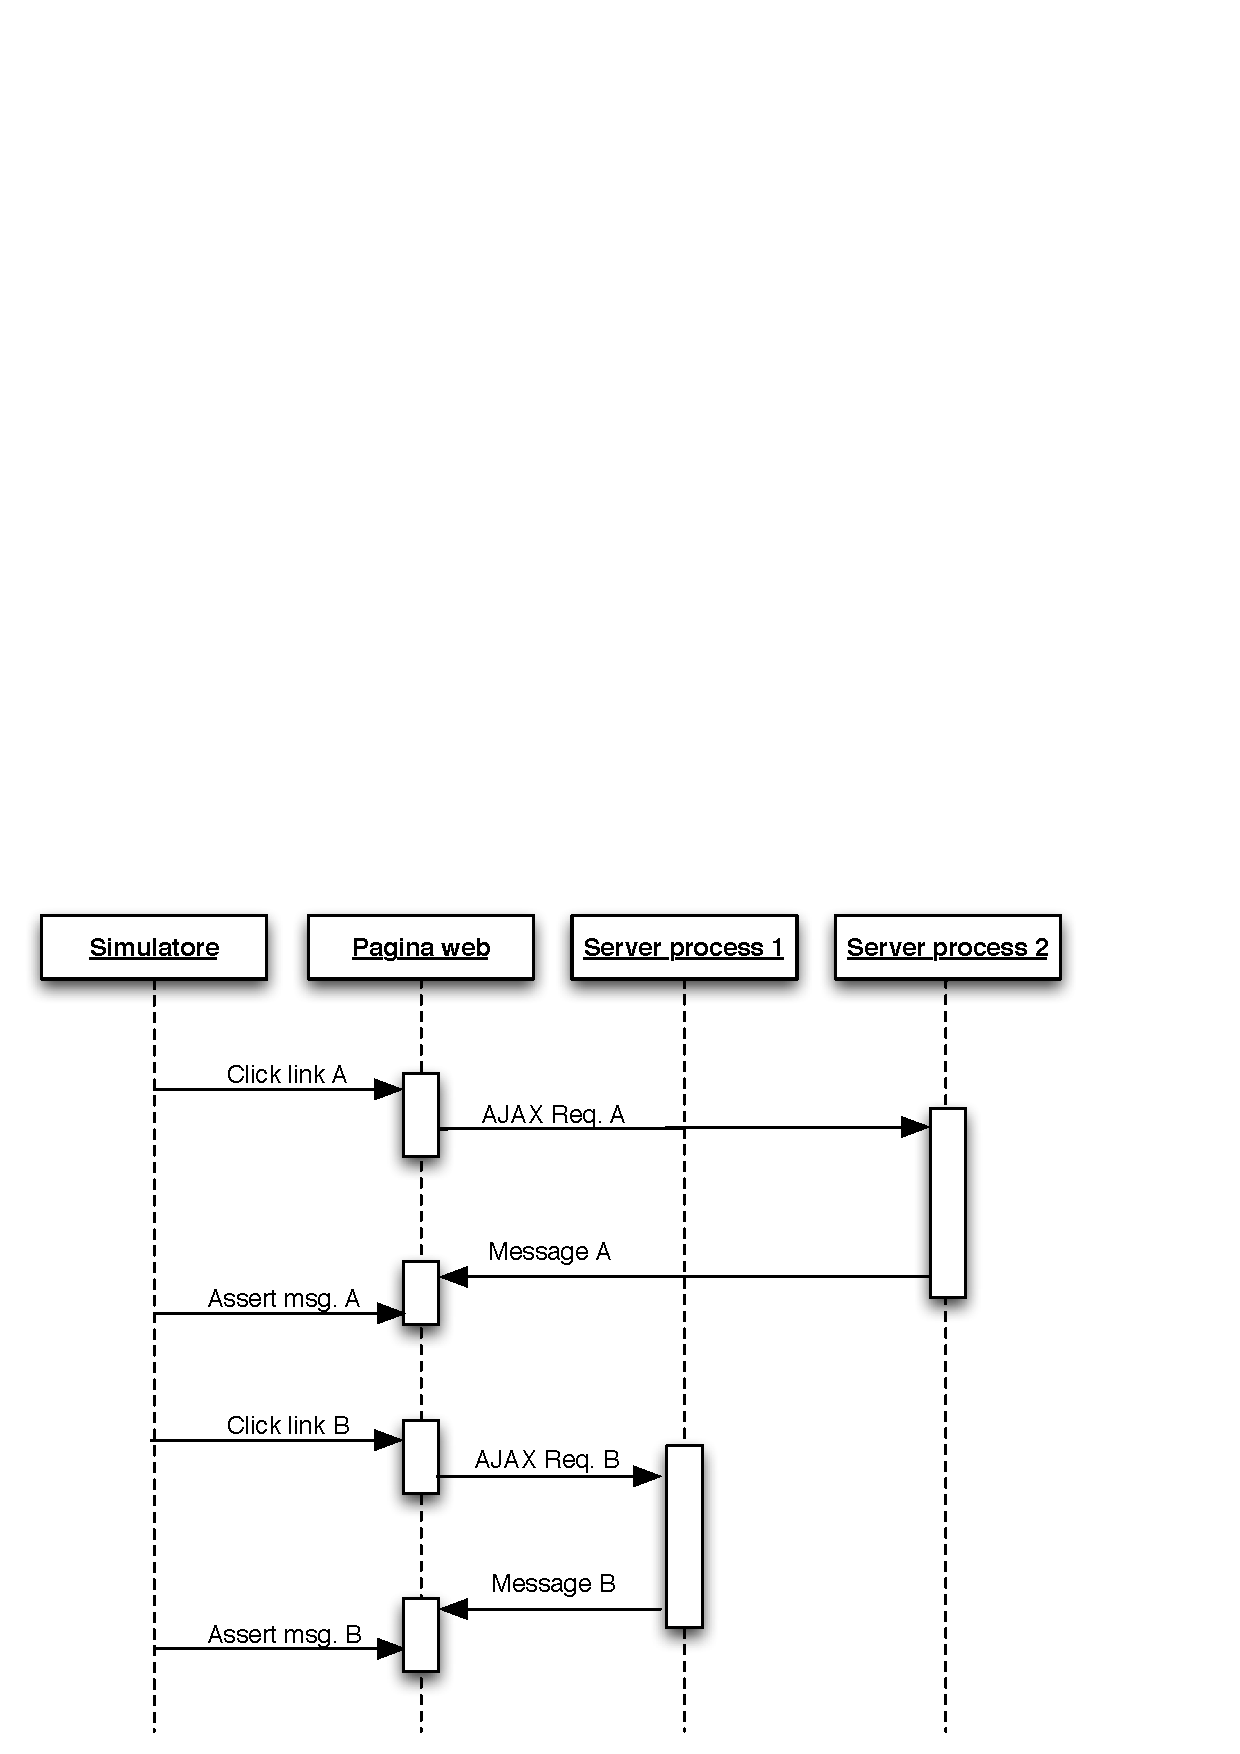
\includegraphics[width=\textwidth]{images/ajax_sync_for_simulation.png}
\caption{Sincronizzazione di richieste parallele durante la simulazione}
\label{fig:ajaxParallelSimulation}
\end{center}
\end{figure}

La figura ~\ref{fig:ajaxParallelSimulation} mostra come il simulatore gestisce uno scenario di test che contempli la presenza di richieste parallele, come quello indicato in figura ~\ref{fig:ajaxSequence}

\subsection{Riproduzione delle azioni}

Il controllo della riproduzione vera e propria delle azioni registrate per il test viene delegato al metodo \verb|play| della classe \verb|Simulator|. Come parametro questo metodo riceve una lista di oggetti di classe \verb|Action|, itera sulla lista e su di  ognuna di esse invoca il metodo \verb|execute|. La logica vera e propria di esecuzione per le azioni e per le asserzioni è contenuta all'interno delle sottoclassi varie della classe \verb|Action|, che espongono l'implementazione specializzata del metodo statico \verb|execute|. Questo metodo viene richiamato passando come parametro un riferimento al simulatore, in modo che l'azione possa utilizzarlo per iniettare codice Javascript nella pagina o per effettuare altre operazioni necessarie.

Il metodo \verb|play| emette poi i segnali \verb|startSimulation| e \verb|endSimulation| rispettivamente all'inizio e alla fine della simulazione, i segnali \verb|startPlayAction|, \verb|endPlayAction| subito prima e subito dopo l'esecuzione di ogni singola azione. La classe della finestra principale intercetta questi eventi e aggiorna l'interfaccia grafica di conseguenza, evidenziando ad esempio l'azione che si sta eseguendo in un dato momento nella vista ad albero.

\section{Modulo actions}

\subsection{Implementazione del Model nel paradigma MVD}

Come è stato descritto in precedenza, il framework Qt implementa il pattern MVD per gestire la visualizzazione dei dati nell'interfaccia grafica. La lista delle azioni viene mostrata all'utente attraverso una TreeView, cui è stato associato un model responsabile di manipolare l'accesso alla struttura dati principale, contenente le azioni registrate che compongono il test. 

La definizione di un model personalizzato ha consentito di avere un controllo maggiore sul modo in cui vengono mostrati i dati nella vista al albero, rispetto all'utilizzo del model generico già implementato all'interno del framework e pronto per essere abbinato alla TreeView nei casi più comuni. 

La struttura dati in cui sono memorizzate le azioni consiste in una lista semplice, una struttura dati già presente in Python attraverso il tipo List. Quando viene registrata una nuova azione, il model fornisce l'interfaccia per inserirla in questa lista, eseguendo poi una serie di operazioni non visibili dall'esterno. Una vista ad albero viene generalmente utilizzata per rappresentare una certa struttura gerarchica presente nei dati. Nel caso dell'applicazione realizzata, la gerarchia da visualizzare consiste in una lista di azioni, considerate come nodi padre, e per ciascuna di essere un'insieme di dettagli, visti come nodi figli della relativa azione. In questo modo l'utente potrà avvantaggiarsi della vista ad albero per visualizzare solo i dettagli di interesse, esplodendo i nodo padre.

Il model deve quindi occuparsi di costruire questa gerarchia, che di per sé non è presente nella struttura dati che memorizza le azioni. Essa infatti è una lista semplice e non un albero, poiché i dettagli di ogni azione sono in realtà memorizzati come proprietà degli oggetti di classe \verb|Action| contenuti nella lista stessa. Il model quindi itera sulla lista delle azioni e da queste costruisce una struttura aggiuntiva ad albero che mappa ciò che la vista associata mostrerà effettivamente. Per i nodi di questo albero viene utilizzata la classe ausiliaria \verb|TreeItem|, che rappresenta un nodo di tipo principale oppure di dettaglio.

La classe \verb|TreeModel| si inserisce nell'architettura MVD del framework ereditando le funzionalità e l'interfaccia dalla classe \verb|QAbstractItemModel|. Per rispettare le convenzioni, essa deve reimplementare alcuni metodi definiti nella classe astratta. 

Nello specifico i metodi \verb|insertRow| e \verb|RemoveRow| si occupano di inserire e rimuovere gli oggetti dalla lista delle azioni e di notificare alla classe della vista il cambiamento dei dati, in modo da sincronizzarne la visualizzazione. Inoltre, quando si eseguono queste operazioni viene aggiornata di conseguenza anche la struttura ad albero interna.

 \lstinputlisting[caption={Costruzione della struttura dati ad albero interna al model}, label=code:buildTreeView]{code/model/convert_to_tree.py}

E' necessario inoltre reimplementare il metodo \verb|index|, poiché esso rende di fatto possibile alla classe \verb|TreeView| l'associazione tra i nodi della struttura ad albero nel model e gli elementi mostrati nella vista. In altre parole, la vista invoca il metodo \verb|index| per sapere quale dato mostrare nelle varie caselle del componente dell'interfaccia.

Una volta acquisito l'indice, la vista richiede al model il dato corrispondente. Per far ciò invoca il metodo \verb|data| del model, passando oltre all'indice anche un parametro indicante il "ruolo", ossia la modalità con cui i dati verranno usati. In base a questo parametro, la vista può richiedere i dati da utilizzare per mostrare il testo, per disegnare lo sfondo oppure un'icona, eccetera. Il model in base al ruolo richiesto fornisce se ne è in grado le informazioni richieste, accedendo alla struttura dati. 

Nel caso particolare dell'applicazione realizzata questo meccanismo viene utilizzato ad esempio per colorare in maniera differente lo sfondo di un elemento della vista al albero che rappresenta un asserzione, a seconda se essa abbia avuto esito positivo o negativo. E' importante notare che, siccome ci si trova ad operare all'interno del paradigma MVD, ogni cambiamento desiderato nelle viste deve essere rispecchiato da un cambiamento nei dati forniti dal model. La cronologia delle azioni che portano ad evidenziare di rosso un'asserzione fallita nella vista ad albero è la seguente:

\begin{enumerate}
\item La classe \verb|Simulator| nel \verb|play| invoca il metodo \verb|execute| sull'oggetto corrispondente all'asserzione corrente
\item L'azione effettua il controllo attraverso il simulatore. L'esito è negativo, la proprietà \verb|Assertion.passed| viene impostata a \verb|False|
\item Viene emesso il segnale \verb|dataChanged| dal model, la vista viene notificata di una modifica nei dati e deve ridisegnare l'elemento corrispondente all'indice ricevuto.
\item La classe \verb|TreeView| richiama il metodo \verb|data| del model indicando l'indice, con ruolo \verb|Qt.DisplayRole|, il model reperisce il dato tramite l'indice e restituisce la stringa da mostrare
\item La classe \verb|TreeView| richiama il metodo \verb|data| con ruolo \verb|Qt.BackgroundRole|, il model reperisce l'azione indicata dall'indice, verifica se è un'asserzione (istanza di \verb|Assertion|) e in tal caso restituisce un oggetto \verb|QBrush| con il quale la vista disegnerà lo sfondo della cella corrispondente. In caso contrario la vista userà le impostazioni standard per lo sfondo.
\end{enumerate}

\lstinputlisting[caption={Implementazione del metodo data per il model delle azioni}, label=code:modelData]{code/model/data_method.py}
 
\subsection{Salvataggio dei test in formato XML}

La classe \verb|TreeModel| si occupa anche di altre due operazioni che interessano i dati, ossia l'esportazione e l'importazione dei test in formato XML. Una volta registrata una sequenza di azioni, l'utente può scegliere di salvarla in un file XML su disco secondo il formato definito dall'applicazione, per poi poterlo recuperare in un secondo momento.

Per il parsing e la generazione del formato XML con codifica UTF-8 è stato utilizzato il package \verb|xml.etree|, che fa parte delle librerie standard fornite dal linguaggio Python, che con poche righe di codice ha consentito di eseguire tutte le operazioni necessarie.

Il metodo \verb|saveToXml| si occupa di creare la rappresentazione in memoria dell'albero XML partendo dalla lista di azioni memorizzate, per poi delegarne la serializzazione e la scrittura su file alle classi della libreria Python. La rappresentazione nel formato XML di ogni tipo di azione disponibile è gestita all'interno delle corrispondenti classi, che devono implementare il metodo \verb|toXML|. In questo modo si evita di accoppiare eccessivamente il codice del model con i dettagli interni di ogni azione.

Un esempio del formato XML utilizzato per rappresentare la sequenza di azioni è riportato nel listato ~\ref{code:xmlFormat} 

\lstinputlisting[language=xml, caption={Formato XML di un test case}, label=code:xmlFormat]{code/model/testcase.xml}

\subsubsection{Azioni ed asserzioni}

Le azioni eseguibili dal simulatore si classificano in due macrocategorie principali: azioni che simulano le operazioni dell'utente sull'interfaccia ed asserzioni che verificano alcuni aspetti circa il corretto funzionamento dell'applicazione.

Ognuna di queste azioni è stata modellata in un'apposita classe, che contiene al suo interno la logica per l'esecuzione. Per facilitare l'implementazione di nuove azioni in aggiunta a quelle già presenti è stata impostata una gerarchia di classi per rappresentare le azioni, in modo da inserire le operazioni comuni nei livelli più alti della linea ereditaria. Tale struttura presenta le seguenti classi:

\begin{description}
\item[ ] La classe di base \verb|Action|, dalla quale ereditano tutte le altre azioni. Questa classe è astratta e definisce l'interfaccia che ogni sottoclasse deve implementare affinché possa essere utilizzata correttamente nell'applicazione.
I tre metodi indispensabili sono il metodo \verb|execute|, che deve contenere la logica per l'esecuzione dell'azione tramite l'istanza della classe \verb|Simulator| passata come parametro, il metodo \verb|fromXML|, che inizializza le proprietà della classe a partire dal nodo XML fornito in ingresso, ed infine il metodo \verb|toXML|, che si occupa di costruire il nodo dell'albero XML per la rappresentazione della classe. Questi ultimi due metodi sono utilizzati per importare ed esportare i test registrati.

\item[ ] La classe astratta \verb|UserAction|, che discende dalla classe \verb|Action| e modella un'interazione dell'utente con l'applicazione web sotto esame. Contiene il codice per gestire le proprietà comuni ad ognuna di esse.

\item[ ] La classe astratta \verb|AssertAction|, con funzioni analoghe alla precedente per le asserzioni.

\item[ ] Le classi che estendono \verb|UserAction|, raggruppate nel modulo \verb|actions.user_actions|, che definiscono una singola azione dell'utente.

\item[ ] Le classi che estendono \verb|AssertAction|, contenute nel modulo \verb|actions.assertions|, che rappresentato i vari tipi di asserzioni supportate dall'applicazione.
 
\end{description}

\begin{figure}[htbp]
\begin{center}
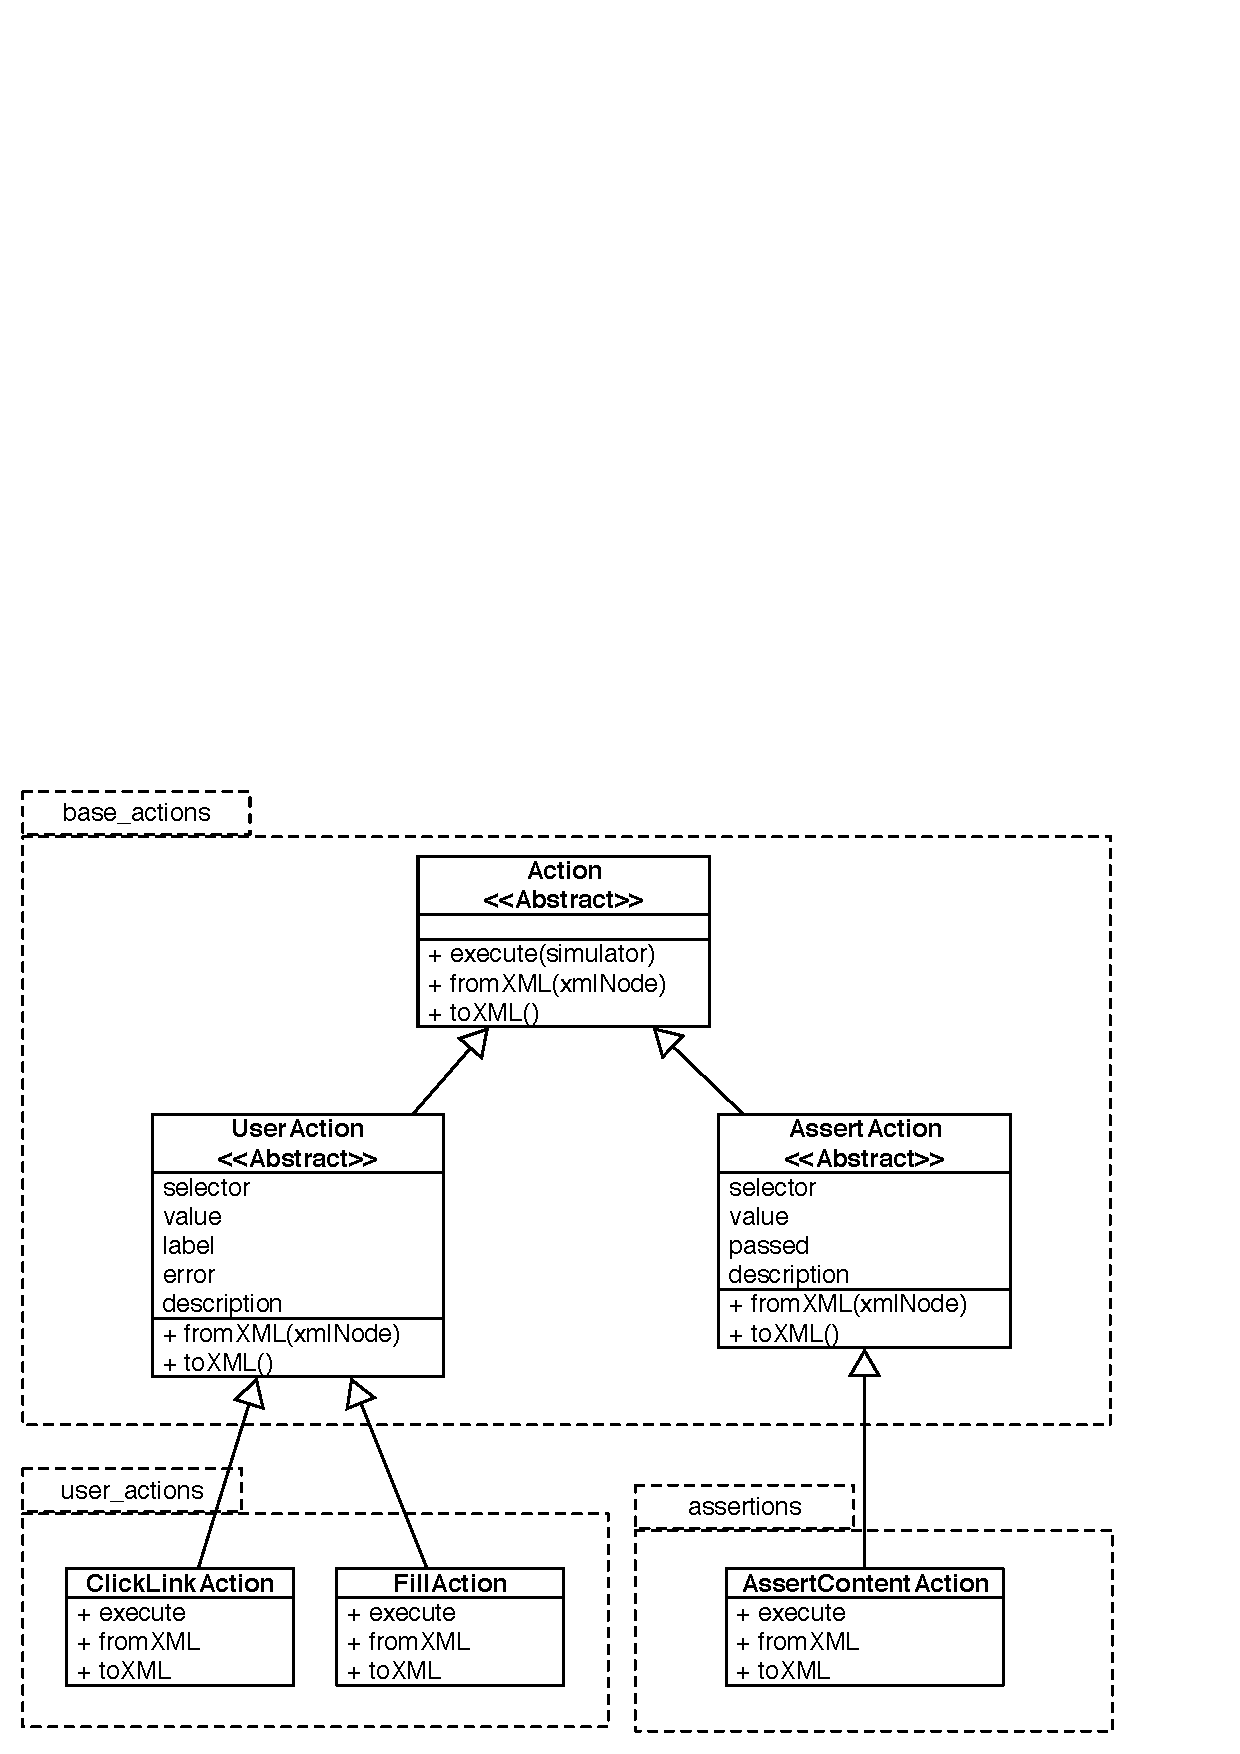
\includegraphics[width=\textwidth]{images/uml_actions.png}
\caption{UML diagram per il package delle azioni}
\label{fig:actionUML}
\end{center}
\end{figure}

Nel listato ~\ref{code:clickLinkAction} viene presentata a titolo esplicativo la classe \verb|ClickLinkAction|, che simula il click dell'utente su di un collegamento ipertestuale. Nel metodo \verb|execute| viene utilizzata l'istanza della classe \verb|Simulator| passata come parametro per eseguire il codice Javascript che simula effettivamente l'evento e per fermare il flusso di esecuzione dei test fino al completamento dell'eventuale richiesta HTTP generata dal click.

\lstinputlisting[language=Python, caption={Dettagli implementativi della classe ClickLinkAction}, label=code:clickLinkAction]{code/actions/click_link_action.py}

Aggiungere nuove azioni disponibili nell'applicazione in un secondo momento non richiede particolari modifiche al codice, oltre all'implementazione della relativa classe. Grazie al sistema di tipizzazione dinamica ("duck typing") tipico del Python e di altri linguaggi non compilati, l'applicazione sarà in grado di utilizzare direttamente le funzionalità esposte dalla nuova classe.

\subsection{La registrazione delle azioni utente}

La cattura delle interazioni tra l'utente e la pagina web viene effettuata usando il meccanismo di gestione degli eventi del DOM. Utilizzando la libreria jQuery è possibile definire delle funzioni di callback, invocate quando un determinato evento raggiunge l'elemento specificato. 

\subsection{DOM event model}

Il motore WebKit utilizzato nel framework Qt adotta la specifica del W3C per il la gestione degli eventi nell'ambito del DOM [http://www.w3.org/TR/DOM-Level-2-Events/events.html], pertanto si è fatto riferimento a queste direttive per identificare una strategia adatta alla cattura degli eventi generati dall'utente. 

In tale specifica vengono definiti le proprietà dell'evento, il modo in cui un evento si propaga nell'albero del DOM e la possibilità di registrare per un nodo dell'albero uno o più \verb|EventListener|, ossia una funzione da eseguire quando l'evento di tipo specificato raggiunge quell'elemento.

La propagazione degli eventi nel DOM viene divisa in due fasi distinte. Durante la prima fase, chiamata "Event capture", l'evento viene propagato in senso discendente nell'albero, dal nodo padre al nodo figlio, fino a raggiungere l'elemento specificato come "target" dell'evento. Le funzioni registrate come EventListener per questa fase possono così manipolare l'oggetto che rappresenta l'evento prima che esso raggiunga il nodo direttamente interessato. E' importante notare che solamente i nodi dell'albero che appartengono alla linea di discendenza del nodo target hanno la possibilità di interagire in questo processo di propagazione. Inoltre, gli EventListener vengono registrati esclusivamente in base alla tipologia dell'evento.

Dopo questa fase discendente, l'evento raggiunge il nodo target e ha inizio la fase di "Event bubbling", simmetrica alla precedente. L'evento infatti risale nella gerarchia dell'albero dal nodo di destinazione fino alla cima e vengono attivati tutti gli EventListener dei nodi interessati da questo percorso e definiti per questa fase, nell'ordine in cui sono stati registrati.

All'interno di un EventListener è inoltre possibile decidere di fermare la propagazione dell'evento oppure decidere di cancellarne l'azione normalmente associata, neutralizzandone di fatto l'effetto.

L'implementazione di WebKit fornisce quindi l'interfaccia Javascript necessaria per intercettare gli eventi nel DOM, tuttavia si è scelto di utilizzare la libreria jQuery poiché essa facilita la gestione degli eventi e offre funzionalità di livello più astratto rispetto all'implementazione nativa, che permettono di trascurare buona parte dei dettagli più difficili da trattare.

\subsection{Registrazione degli eventi}

Attraverso il metodo \verb|jQuery.bind| viene registrata una funzione di callback per il tipo di evento specificato come parametro. Grazie all'interfaccia fluente della libreria, questo metodo è invocabile direttamente su un insieme di oggetti del DOM selezionati. In questo caso la funzione di callback sarà associata a tali nodi del DOM e quindi invocata quando l'evento del tipo specificato li raggiungerà nel suo percorso di propagazione. E' da tenere presente che jQuery permette di associare un event listener solo per la fase di "Event bubbling" e non per la fase di "Event capture". Questa limitazione non ha però avuto ripercussioni nell'applicazione ricercata. 

Per intercettare gli eventi dell'utente si sono quindi associate le funzioni di callback agli elementi di interesse:

\begin{enumerate}
\item Per i campi di testo si è registrato l'event handler in corrispondenza dell'evento jQuery \verb|blur|, generato quando l'elemento specificato perde la proprietà di focus. Ciò accade quando l'utente interagisce con un altro elemento della pagina, segnalando di fatto di aver terminato la digitazione dell'input.

\item Per i collegamenti ipertestuali, le caselle di selezione, i radio button ed i bottoni dei form si intercetta l'evento \verb|click|.

\item Per i menù a tendina l'evento di interesse è di tipo \verb|change|, che si verifica quando l'utente modifica il valore selezionato.

\end{enumerate}

Il codice che definisce queste funzioni viene iniettato nella pagina web dalla classe \verb|Simulator|, secondo le modalità descritte in precedenza. Grazie al canale di comunicazione instaurato dal framework PyQt tra contesto Python e contesto Javascript, all'interno di ognuna di esse viene invocato il rispettivo metodo della classe Python \verb|Logger|. Essa si occupa di creare l'istanza corretta della classe \verb|UserAction| in base all'evento che è stato catturato e di memorizzarla nella struttura dati dell'applicazione.

\lstinputlisting[language=Javascript, caption={Esempio di codice per la cattura degli eventi in Javascript}, label=code:eventHandlers]{code/actions/log_select.js}

Affinché l'evento sia riproducibile in un secondo momento, bisogna memorizzare un selettore all'elemento interessato. Per fare ciò viene usato un algoritmo di generazione del selettore CSS per l'elemento corrente descritto in seguito. Il suo ruolo è fondamentale in fase di riproduzione poiché tramite grazie ad esso l'elemento da cui far partire l'evento verrà recuperato nella pagina. 

Le funzioni di callback per gli eventi si interessano anche di reperire informazioni aggiuntive da presentare all'utente ai fini di una migliore leggibilità dei test registrati. Ad esempio, nel caso dei collegamenti ipertestuali viene estratto il testo contenuto nel tag anchor, mentre nel caso di un campo di input viene reperito, se presente, il contenuto del tag label ad esso associato, che fornisce indicazioni sul dato da inserire. Grazie a questi accorgimenti, i passi registrati dallo strumento sono comprensibili anche senza avere competenze tecniche particolari, come mostrato in figura ~\ref{fig:actionNotes}.

\begin{figure}[htbp]
\begin{center}
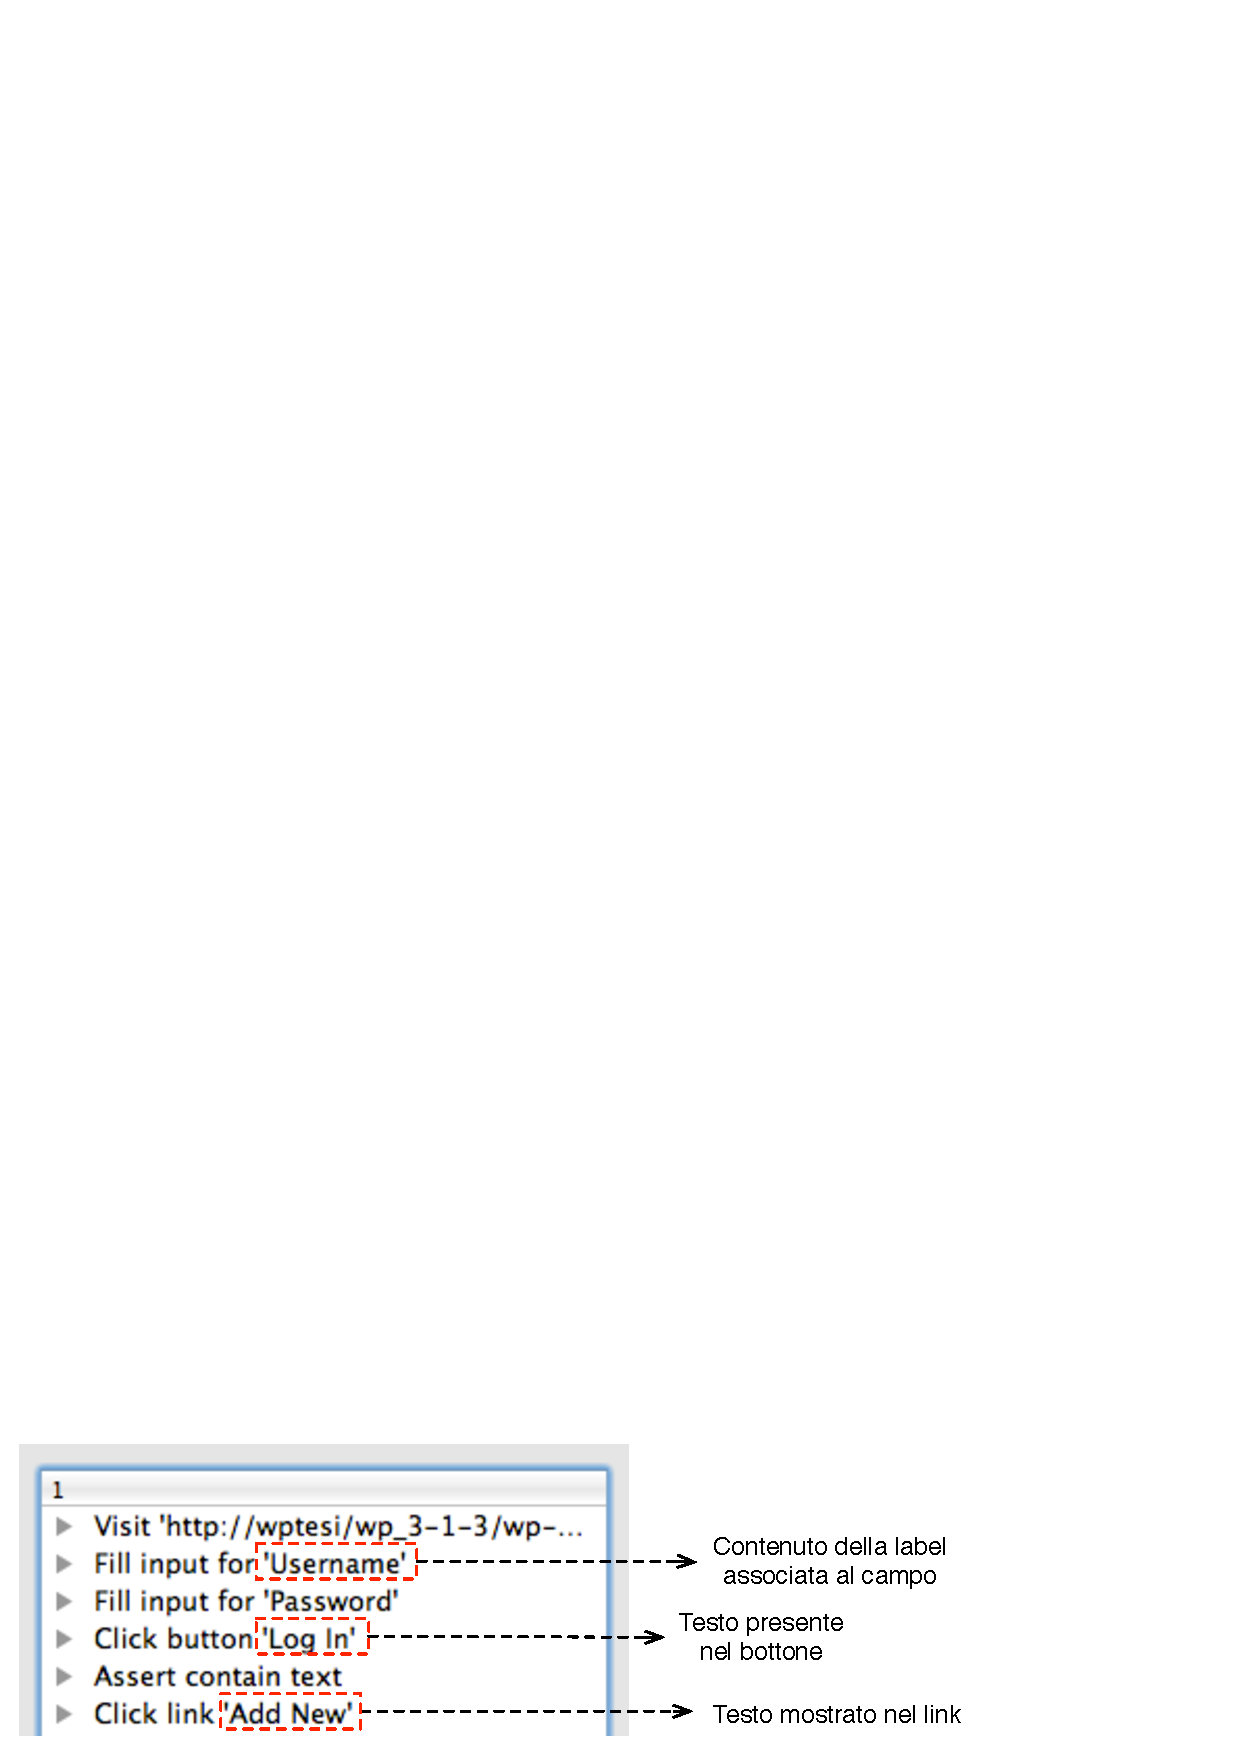
\includegraphics[width=\textwidth]{images/action_notes.png}
\caption{Lista delle azioni registrate mostrata all'utente nell'interfaccia grafica}
\label{fig:actionNotes}
\end{center}
\end{figure}

Si è rivelata di notevole interesse inoltre la funzione \verb|jQuery.live|, qualora l'applicazione web su cui si stanno effettuando i test faccia uso di richieste AJAX. In questi casi è frequente che il DOM venga modificato una volta terminata la richiesta, ad esempio creando nuovi nodi per mostrare nella pagina i dati ricevuti dal server. 

Siccome questi nuovi elementi non erano presenti nel DOM nel momento in cui è stato iniettato il codice Javascript, gli event listener per questi nodi non sono stati registrati e risulterebbe impossibile intercettare gli eventi che li interessano. Utilizzando la funzione \verb|jQuery.live| invece che \verb|jQuery.bind|, viene registrato un event listener speciale per il nodo radice dell'albero DOM. Quando l'evento si verifica esso viene propagato dal basso verso l'alto durante la fase di "event bubbling" e poiché non sono associati event listener al nodo del DOM appena inserito, esso raggiunge il nodo radice, dove viene intercettato dall'event listener registrato tramite \verb|.live|. A questo punto viene verificato che l'elemento target dell'evento coincida con quello specificato per \verb|live| e in caso positivo si procede all'esecuzione del codice di gestione dell'evento. Siccome quest'ultimo passaggio non viene effettuato fino a che l'evento non si verifica, gli elementi che corrispondono al selettore indicato rispondono comunque all'evento, anche se aggiunti al DOM in un secondo momento.

Uno scenario tipico viene rappresentato in figura ~\ref{fig:liveEventCase}, dove è necessario poter continuare il test dell'applicazione cliccando su link aggiunto alla pagina dopo la richiesta asincrona.

\begin{figure}[htbp]
\begin{center}
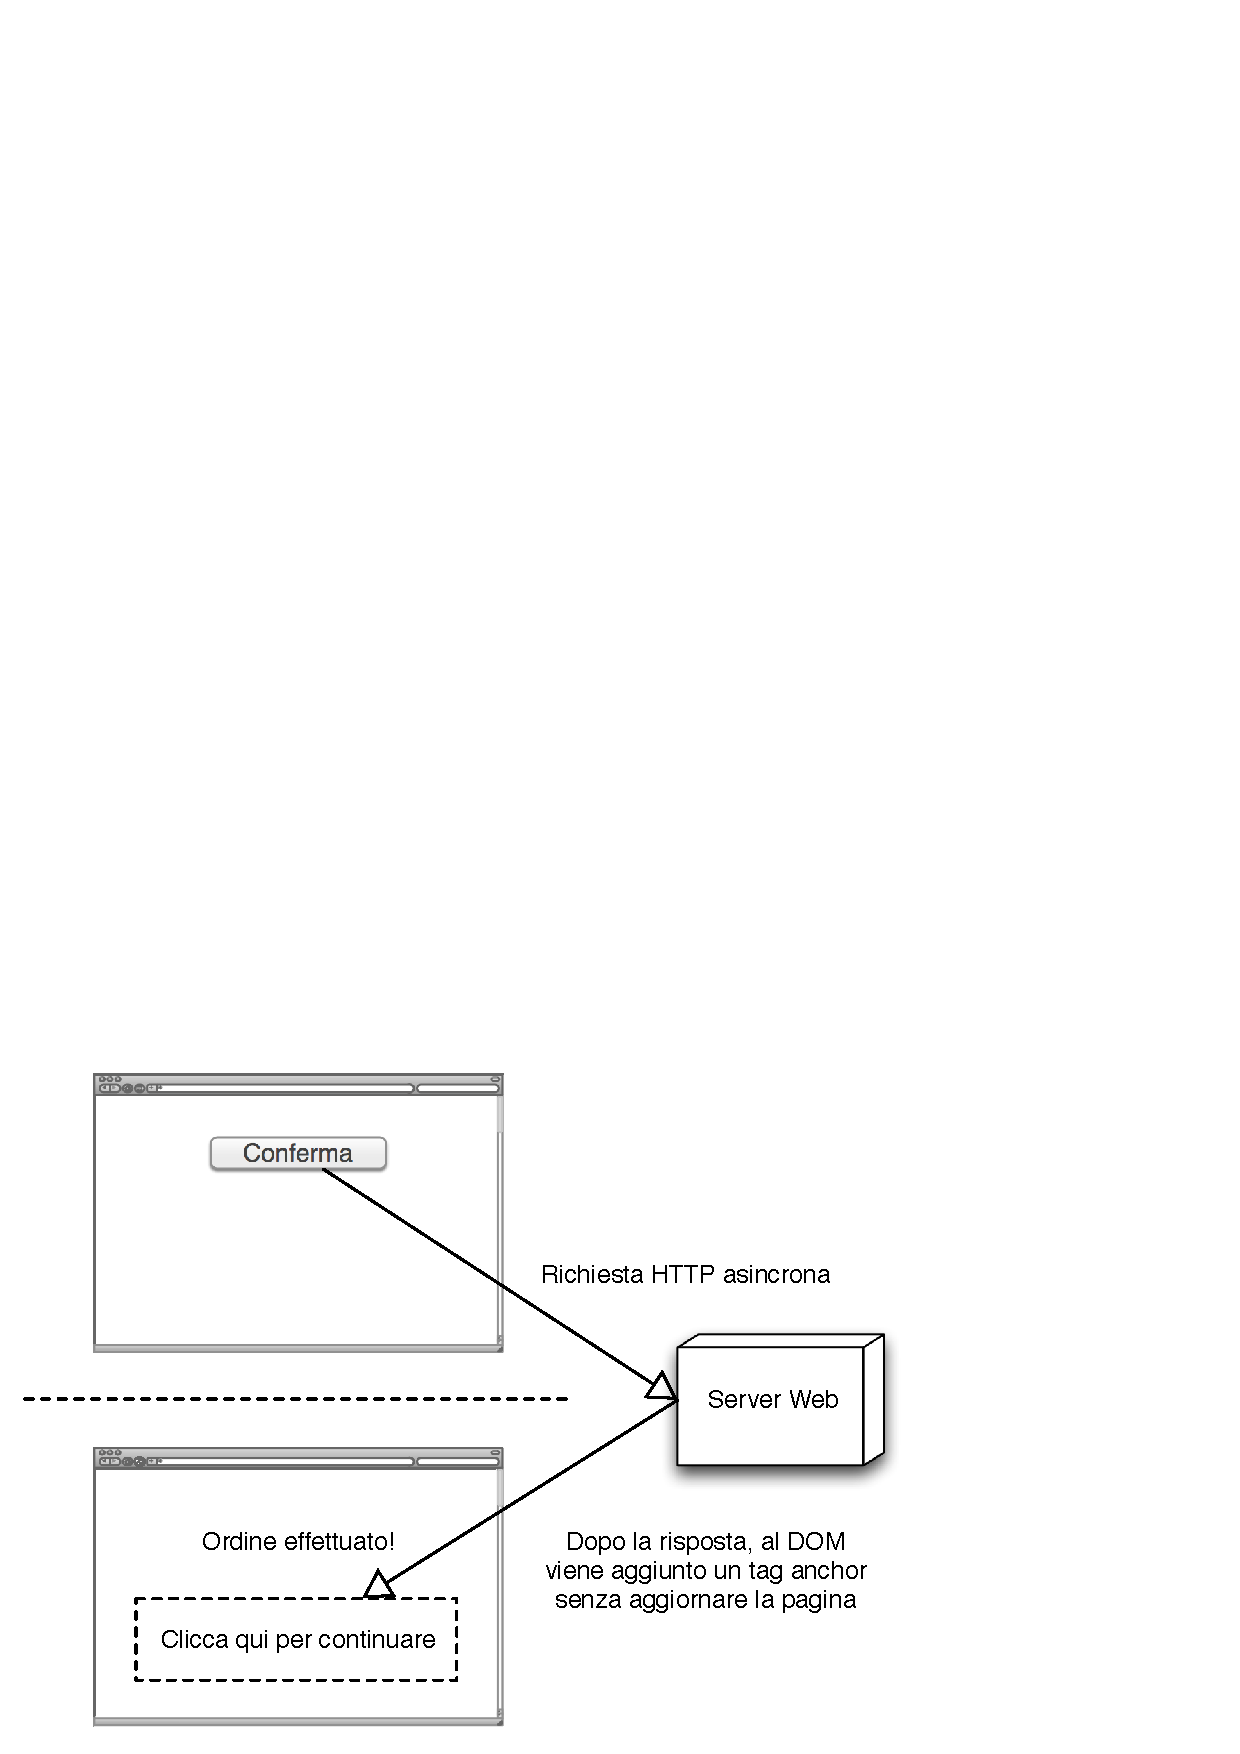
\includegraphics[width=\textwidth]{images/live_event_case.png}
\caption{Esempio di scenario che contempla la modifica del DOM}
\label{fig:liveEventCase}
\end{center}
\end{figure}

%TODO: solo alcuni eventi sono registrati, spiegare ?

\subsection{Riproduzione degli eventi}

Una volta che le azioni compiute dall'utente sulla pagina web sono state registrate mediante la strategia descritta nel paragrafo precedente, è necessario poterle riprodurre in maniera programmatica per simulare l'interazione dell'utente durante la simulazione del test.

Per sintetizzare gli eventi sono state considerate ed implementate due strategie alternative, che verranno ora analizzate nel dettaglio.

\subsubsection{Eventi Javascript}

La soluzione che si è rivelata più semplice consiste nel riprodurre gli eventi tramite codice Javascript, in maniera simmetrica a come essi vengono registrati. Per la scrittura del codice apposito si è tratta in parte ispirazione dal framework YUI Library, rilasciata da Yahoo con licenza BSD, la quale contiene un modulo per la simulazione degli eventi. 

Come punto di partenza si è utilizzata l'API definita dalla specifica DOM Event del W3C, la quale definisce i metodi \verb|createEvent| e \verb|dispatchEvent| per creare un evento di un dato tipo e per avviare la sua propagazione del DOM. Attraverso questi metodi è perciò possibile sintetizzare tutte le tipologie di eventi definite nella specifica, personalizzandone se necessario le proprietà.

Il codice Javascript che si occupa di generare gli eventi è stato implementato come un plugin per la libreria jQuery all'interno del file \verb|jquery.simulate.js| così da integrarne l'utilizzo con l'interfaccia fluente di jQuery. Grazie all'architettura dei plugin, i metodi definiti per creare gli eventi sono invocabili direttamente su di una collezione di nodi del DOM selezionata tramite la sintassi standard di jQuery.

\lstinputlisting[language=Javascript, caption={Creazione di un evento del mouse in Javascript}, label=code:jsMouseEvent]{code/actions/create_event.js}

Il plugin per la simulazione degli eventi viene iniettato nella pagina dal simulatore subito dopo il termine del caricamento e classi in Python ne possono richiamare le funzionalità all'interno del rispettivo metodo \verb|execute| utilizzando come intermediario la classe \verb|Simulator|. 

Questo meccanismo di sintesi è stato utilizzato per riprodurre gli eventi legati al mouse, come il click o lo spostamento del puntatore sopra un determinato elemento. L'inserimento di una sequenza di caratteri all'interno di un campo di testo e la sezione di un'opzione da un menù a tendina sono stati invece implementati attraverso il metodo \verb|val()| dell'API jQuery, che imposta il valore del campo di input al parametro passato. Questa scelta ha permesso di semplificare la simulazione di questi eventi, che altrimenti avrebbero dovuto essere realizzati attraverso la combinazione di una serie di eventi. E' infatti possibile riprodurre l'inserimento di una stringa in un campo di testo anche attraverso la propagazione di un evento di tipo \verb|keyPress| per ogni carattere della stringa immessa.

I due principali vantaggi di questo approccio sono dati dalla facilità di creare eventi tramite codice Javascript e dal fatto che durante questa operazione ci si trova già direttamente nel contesto del DOM della pagina. Ciò rende più semplice migliorare l'implementazione adottata interagendo se necessario con gli altri elementi. Inoltre, è possibile avvantaggiarsi direttamente dell'uso di jQuery per la manipolazione semplificata degli eventi.

Di contro, lo svantaggio principali risiede nel livello di accuratezza della simulazione che questo metodo fornisce. Quando l'utente effettua un click su di un link di fatto non viene generato un unico evento, bensì si originano una serie di eventi collaterali subito prima e subito dopo l'azione che l'utente ha intenzione di compiere. Nel caso dell'esempio corrente, lo spostamento del mouse sull'elemento \verb|anchor| ne scatena prima di tutto l'evento \verb|onmouseover|. Ancora prima del click vero e proprio, a seconda del tipo l'elemento può ottenere lo stato di focus, che provoca l'omonimo evento.

Nel caso di applicazioni più complesse, a questi eventi collaterali vengono associati degli event listener per implementare alcune funzionalità importanti, come nel caso dell'autocompletamento per un campo di input. A seconda di come sono stati implementati questi dettagli, potrebbe quindi non essere sufficiente simulare un solo evento per riprodurre in maniera sufficientemente verosimile il reale comportamento dell'utente. Tuttavia, nei casi di studio esaminati questo problema non si è mai presentato in maniera tale da compromettere l'esecuzione dei test.

\subsubsection{Eventi nativi}

La seconda strategia analizzata per la simulazione degli eventi nell'applicazione web si avvantaggia degli eventi nativi. 

E' opportuno ricordare che anche l'applicazione realizzata all'interno del framework Qt implementa una gestione interna degli eventi, concettualmente simile a quella presentata per il DOM. Il componente grafico QWebView, che disegna sullo schermo la pagina web caricata, è soggetto come ogni altro widget al meccanismo di propagazione degli eventi. Pertanto quando l'utente effettua un click sul widget QWebView l'evento viene intercettato e quest'ultimo innesca poi la creazione del relativo evento nel DOM della pagina. 

Anziché sintetizzare l'evento di interesse direttamente nel contesto del DOM, si è quindi pensato di sfruttare il controllo esercitabile sull'ambiente esterno per spostare la simulazione dell'evento ad un livello decisamente più basso, molto più vicino a quello del sistema operativo sottostante. In questo modo la simulazione dell'evento è decisamente più accurata, poiché il componente \verb|QWebView| riceve degli eventi del tutto analoghi a quelli che riceverebbe dal loop principale dell'applicazione, provenienti dal sistema operativo, e li riporta in maniera nativa nel contesto della pagina web. Dal punto di vista di quest'ultima non è pertanto possibile distinguere tra un evento reale ed uno simulato attraverso tale strategia in maniera pratica. In figura ~\ref{fig:nativeEvents} è riportato lo schema a blocchi dei componenti interessati durante la simulazione nativa degli eventi.

\begin{figure}[htbp]
\begin{center}
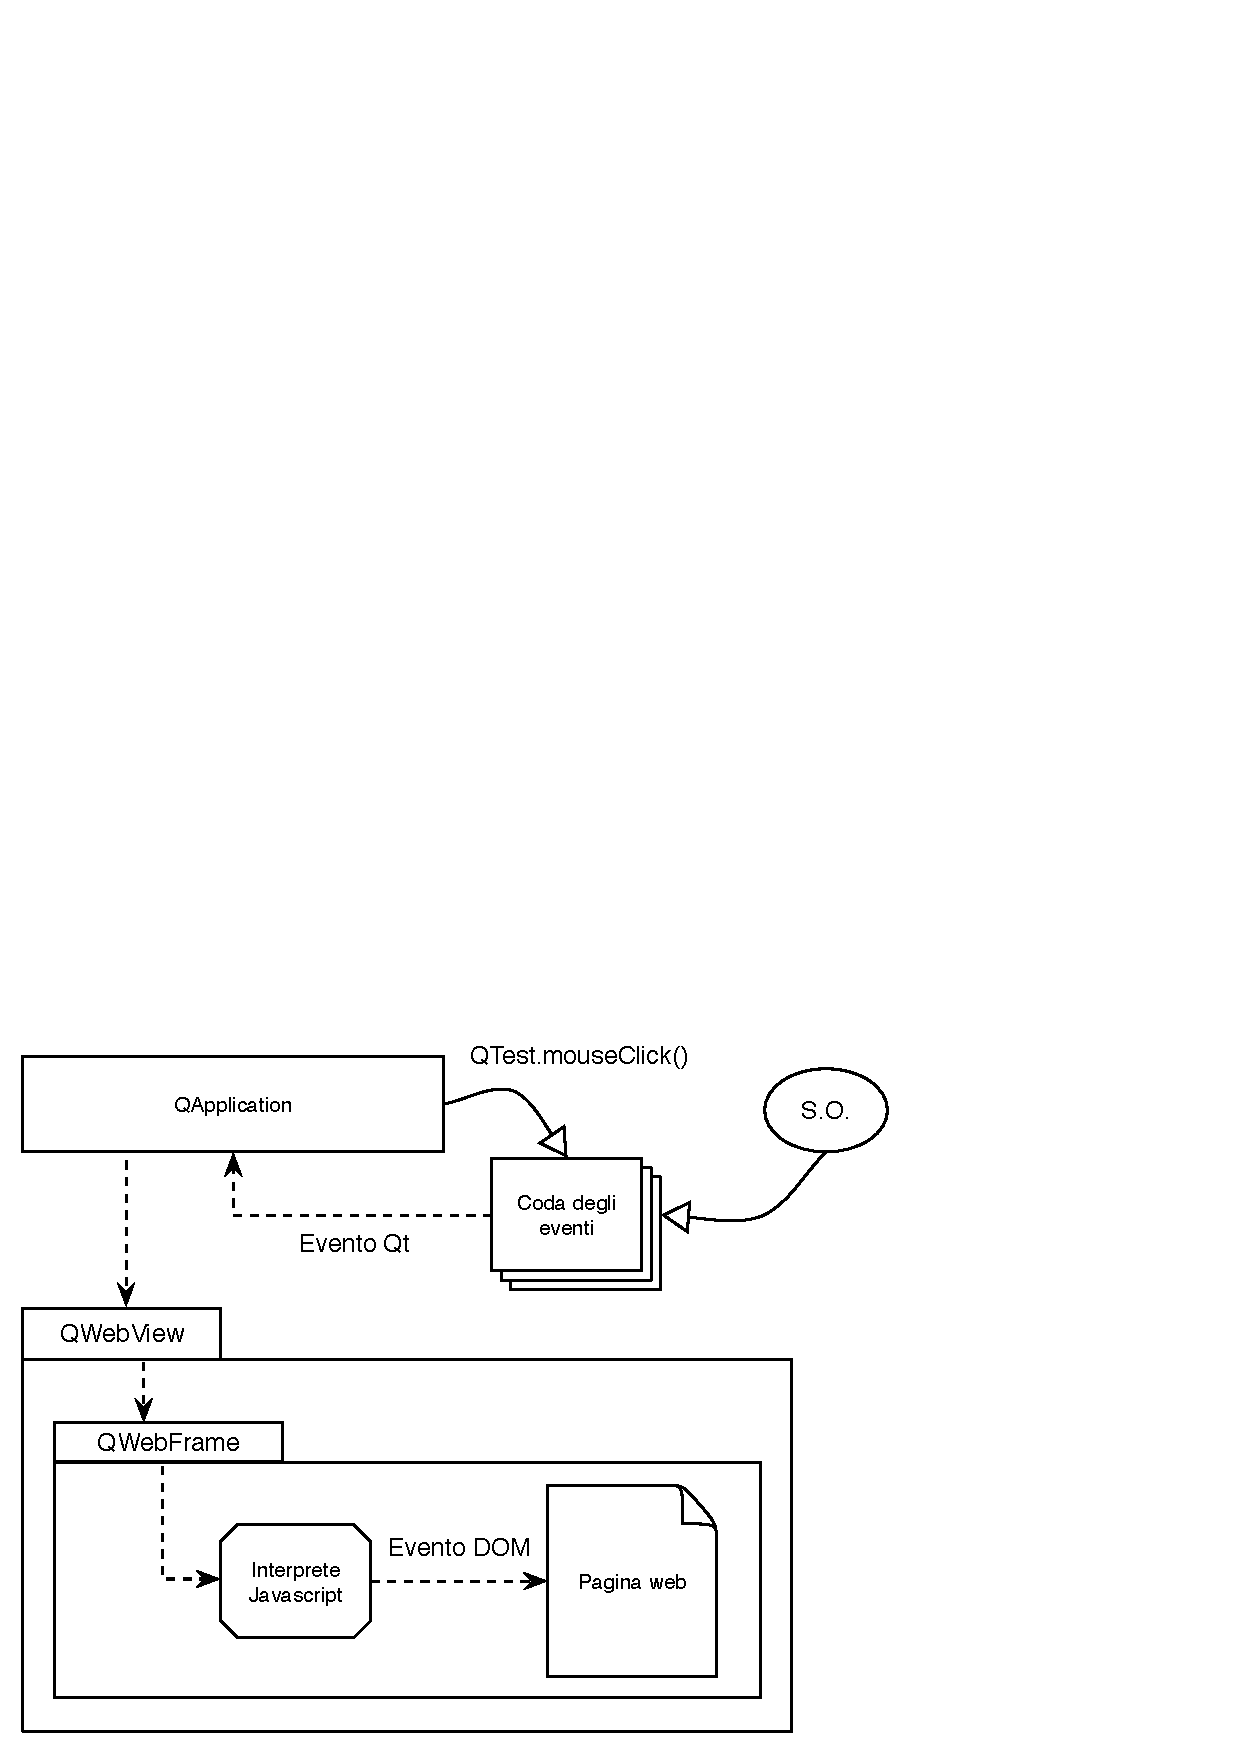
\includegraphics[width=\textwidth]{images/native_events.png}
\caption{Flusso degli eventi per la simulazione nativa}
\label{fig:nativeEvents}
\end{center}
\end{figure}

Per inviare all'applicazione eventi definiti dal framework Qt si possono utilizzare i metodi \verb|QCoreApplication::sendEvent| e \verb|QCoreApplication::postEvent|, che, con alcune differenze interne, inseriscono un oggetto di tipo \verb|QtEvent| nella coda degli eventi dell'applicazione, specificando quale widget deve risultare come primo destinatario di tale evento. L'utilizzo di tali metodi, tentato come primo approccio, ha comportato una serie di problematiche non banali che hanno quindi portato alla ricerca di una soluzione alternativa.

L'attenzione si è quindi spostata sul modulo \verb|QTest| del framework, concepito per facilitare l'esecuzione di test sulle interfacce grafiche realizzate con Qt. Per questo scopo il modulo offre dei metodi per la simulazione degli eventi, che hanno consentito di aggirare agevolmente gli ostacoli incontrati durante il primo approccio al problema.

Nello specifico sono stati utilizzati principalmente i metodi \verb|QTest:.mouseMove| e \verb|QTest:.mouseClick| per simulare le interazioni principali con il componente \verb|QWebView|, come mostrato nel listato ~\ref{code:nativeClickLink}. In questo estratto si può osservare come l'azione di click su di un link venga riprodotta simulando prima lo spostamento del mouse sul nodo del DOM e poi l'effettivo click.

\lstinputlisting[language=Python, caption={Implementazione nativa dell'azione ClickLink}, label=code:nativeClickLink]{code/actions/click_link_native.py}

Come primo parametro viene indicata l'istanza di classe \verb|QWidget| a cui deve essere recapitata per prima la notifica dell'evento. L'altro parametro comune rappresenta invece le coordinate dello schermo alle quali si deve verificare l'evento simulato, indicate tramite un oggetto di classe \verb|QPoint|.

Per ricavare le coordinate del nodo del DOM destinatario dell'evento si è seguito il seguente approccio. Il simulatore esegue del codice Javascript che richiama il metodo \verb|jQuery.offset| sul nodo selezionato, il quale restituisce l'ascissa e l'ordinata dell'elemento in base alla distanza dal margine sinistro e da quello superiore della pagina. Successivamente viene istanziato un oggetto di classe \verb|QPoint| con i valori ottenuti. 

A questo punto è necessario convertire le coordinate dell'elemento relative al componente \verb|QWebView| al sistema sistema di riferimento della finestra applicativa, in modo da identificare correttamente la posizione utilizzata per simulare l'evento. 

\lstinputlisting[language=Python, caption={Coordinate del nodo DOM interessato dalla simulazione}, label=code:elementPosition]{code/actions/element_position.py}

\chapter{Algoritmi di selezione degli elementi}

\section{Considerazioni iniziali e prerequisiti}

Al momento della registrazione delle azioni è indispensabile poter generare un selettore CSS che permetta di identificare in maniera univoca l'elemento interessato dall'interazione, per potervi accedere in fase di riproduzione. In aggiunta, il selettore individuato dovrebbe garantire una certa flessibilità ai cambiamenti che possono avvenire nel DOM durante il successivo sviluppo dell'applicazione, per non ritrovarsi con un insieme di test troppo fragili.
Allo stesso tempo però è necessario raggiungere un compromesso accettabile tra la resistenza alle variazioni e l'accuratezza delle verifiche, in modo che queste ultime permettano effettivamente di rivelare i problemi che si presentano.

La soluzione proposta parte da alcune considerazioni di partenza, basate principalmente sulla propria esperienza e sui criteri generali considerati come migliore prassi nella realizzazione di pagine web dinamiche, descritte di seguito. Tali punti non sono da considerarsi come vincoli necessari per il funzionamento dell'algoritmo, ma piuttosto come un'insieme di condizioni sotto le quali esso può esprime il suo funzionamento ottimale. 

\subsection {Validazione della sintassi HTML}

I risultati dell'algoritmo sono da considerarsi prevedibili solamente nel caso che il codice HTML della pagina web su cui esso viene applicato sia valido secondo la DTD dichiarata. Questa condizione presuppone che l'albero del DOM possa essere costruito in maniera corretta e che vengano eliminate possibili ambiguità, difficili da gestire in fase di analisi. I browser tentano di correggere gli errori di sintassi più comuni e spesso i problemi non sono così evidenti ad una semplice verifica visuale del contenuto mostrato. 

In particolare, l'algoritmo sfrutta in maniera intensiva la presenza e la distribuzione del l'attributo id per determinare quali elementi del DOM siano meno soggetti a potenziali cambiamenti. E' quindi importante che l'attributo id venga utilizzato in maniera corretta, secondo le specifiche del W3C, evitandone per esempio la duplicazione. Se per generare le pagine si utilizzano sistemi di gestione dei contenuti (CMS) spesso non si ha il controllo completo sugli attributi id assegnati ai nodi, perciò in tali casi è bene assicurarsi che l'attributo venga adoperato in maniera adeguata.

Per ottenere i migliori risultati è quindi sempre consigliabile assicurarsi di validare il codice HTML delle pagine sotto esame attraverso uno strumento come il W3C Validator [http://validator.w3.org]. Le specifiche dettate da questa organizzazione sono state infatti utilizzate per stabilire un'insieme omogeneo di regole su cui fondare la strategia dell'algoritmo.

Se questo requisito non viene rispettato, potrebbe essere possibile perdere molti dei vantaggi forniti dall'algoritmo in termini di flessiblità ai cambiamenti strutturali delle pagine.

\subsection {Utilizzo dei tag HTML in maniera semantica}

Ogni tipologia di tag HTML disponibile è stato pensato per trasmettere un significato semantico preciso ai contenuti della pagina, e non solamente per regolarne l'aspetto con cui esso viene presentato. La scrittura di codice HTML semantico è oramai diventata una prassi consolidata nello sviluppo di applicazioni web moderne poiché i benefici ottenibili sono molteplici ed interessano ambiti diversi, dalla mantenibilità del codice all'indicizzazione sui motori di ricerca, passando per l'accessiblità.

L'algoritmo proposto cerca di sfruttare per quanto possibile il significato semantico attribuito ai vari elementi della pagina per reperire ulteriori informazioni e stabilire un selettore che tenga in considerazione le porzioni di pagina soggette a modifiche con maggiore probabilità.

Un uso attento della semantica implica generalmente anche la presenza di un minor numero di tag HTML nella pagina, ossia di un albero del DOM più compatto. Ciò favorisce evidentemente la robustezza dei test sull'interfaccia, sia perché riduce il numero di componenti che possono variare, sia perché i selettori generati sono più semplici ed effettivi. Per gli stessi motivi è opportuno affidare quanto più possibile ai fogli di stile la presentazione del contenuto, senza ricorrere ove non necessario all'aggiunta di codice di markup aggiuntivo per fini prettamente grafici.

In merito a questo criterio non possono esistere regole deterministiche e schemi prefissati da seguire. E' quindi responsabilità di chi si occupa dello sviluppo dell'interfaccia utente dell'applicazione web la scrittura di codice che faciliti la fase di verifica. L'algoritmo proposto cerca infatti di fornire supporto per stabilire la strategia di selezione degli elementi, ma l'uso di uno strumento automatico può sfruttare ma non può sostituire il lavoro svolto a monte per scrivere codice di qualità. Questa affermazione d'altronde è valida nell'ambito dei test in ogni dominio: più il codice sotto esame è ben organizzato, più sarà facile verificarne il funzionamento dall'esterno.

\section{Idee ed ipotesi di partenza}

Il funzionamento dell'algoritmo fonda le sue basi su di un modello empirico e non su concetti dimostrabili a priori, poiché le differenti casistiche che si presentano esaminando applicazioni web reali sono in numero potenzialmente infinito. Pertanto i punti di partenza sono stati forniti dalla propria esperienza nella realizzazione di pagine e di applicazioni web utilizzando le tecnologie più recenti, e dall'osservazione diretta di casi significativi.

Gli spunti raccolti hanno contribuito a definire una serie di criteri adattabili alle situazioni comuni, attraverso i quali l'algoritmo tenta di risolvere i problemi tipici presenti nel test di applicazioni web. L'obiettivo principale è riuscire a stabilire un selettore CSS che identifichi l'elemento corretto nonostante le possibili modifiche che interessino i suoi attributi, quelli dei nodi appartenenti alla sua linea gerarchica e il suo posizionamento nel DOM. A seguire viene presentato un elenco delle variazioni più comuni, per chiarificare i concetti esposti fino ad ora.

\subsection {Schemi tipici di variazioni nel DOM}

Nella figura ~\ref{fig:domMod} sono presentati i principali schemi individuati secondo i quali avvengono le variazioni nel DOM durante il processo incrementale di sviluppo dell'applicazione web. Nei diagrammi sono evidenziati in arancione i nodi di interesse ai fini del test. 

Le modifiche rappresentate non pregiudicano in linea di massima il funzionamento della pagina in esame: si pensi ad esempio al caso comune in cui si aggiunga un tag div che funge da semplice contenitore, oppure all'aggiunta di una o più classi per ragioni stilistiche. E' quindi importante che il selettore tenga in considerazione queste potenziali variazioni in modo che l'elemento interessato sia reperibile anche seguito ad esse, pena il fallimento del test senza un effettivo difetto funzionale.

\begin{figure}[htbp]
\begin{center}
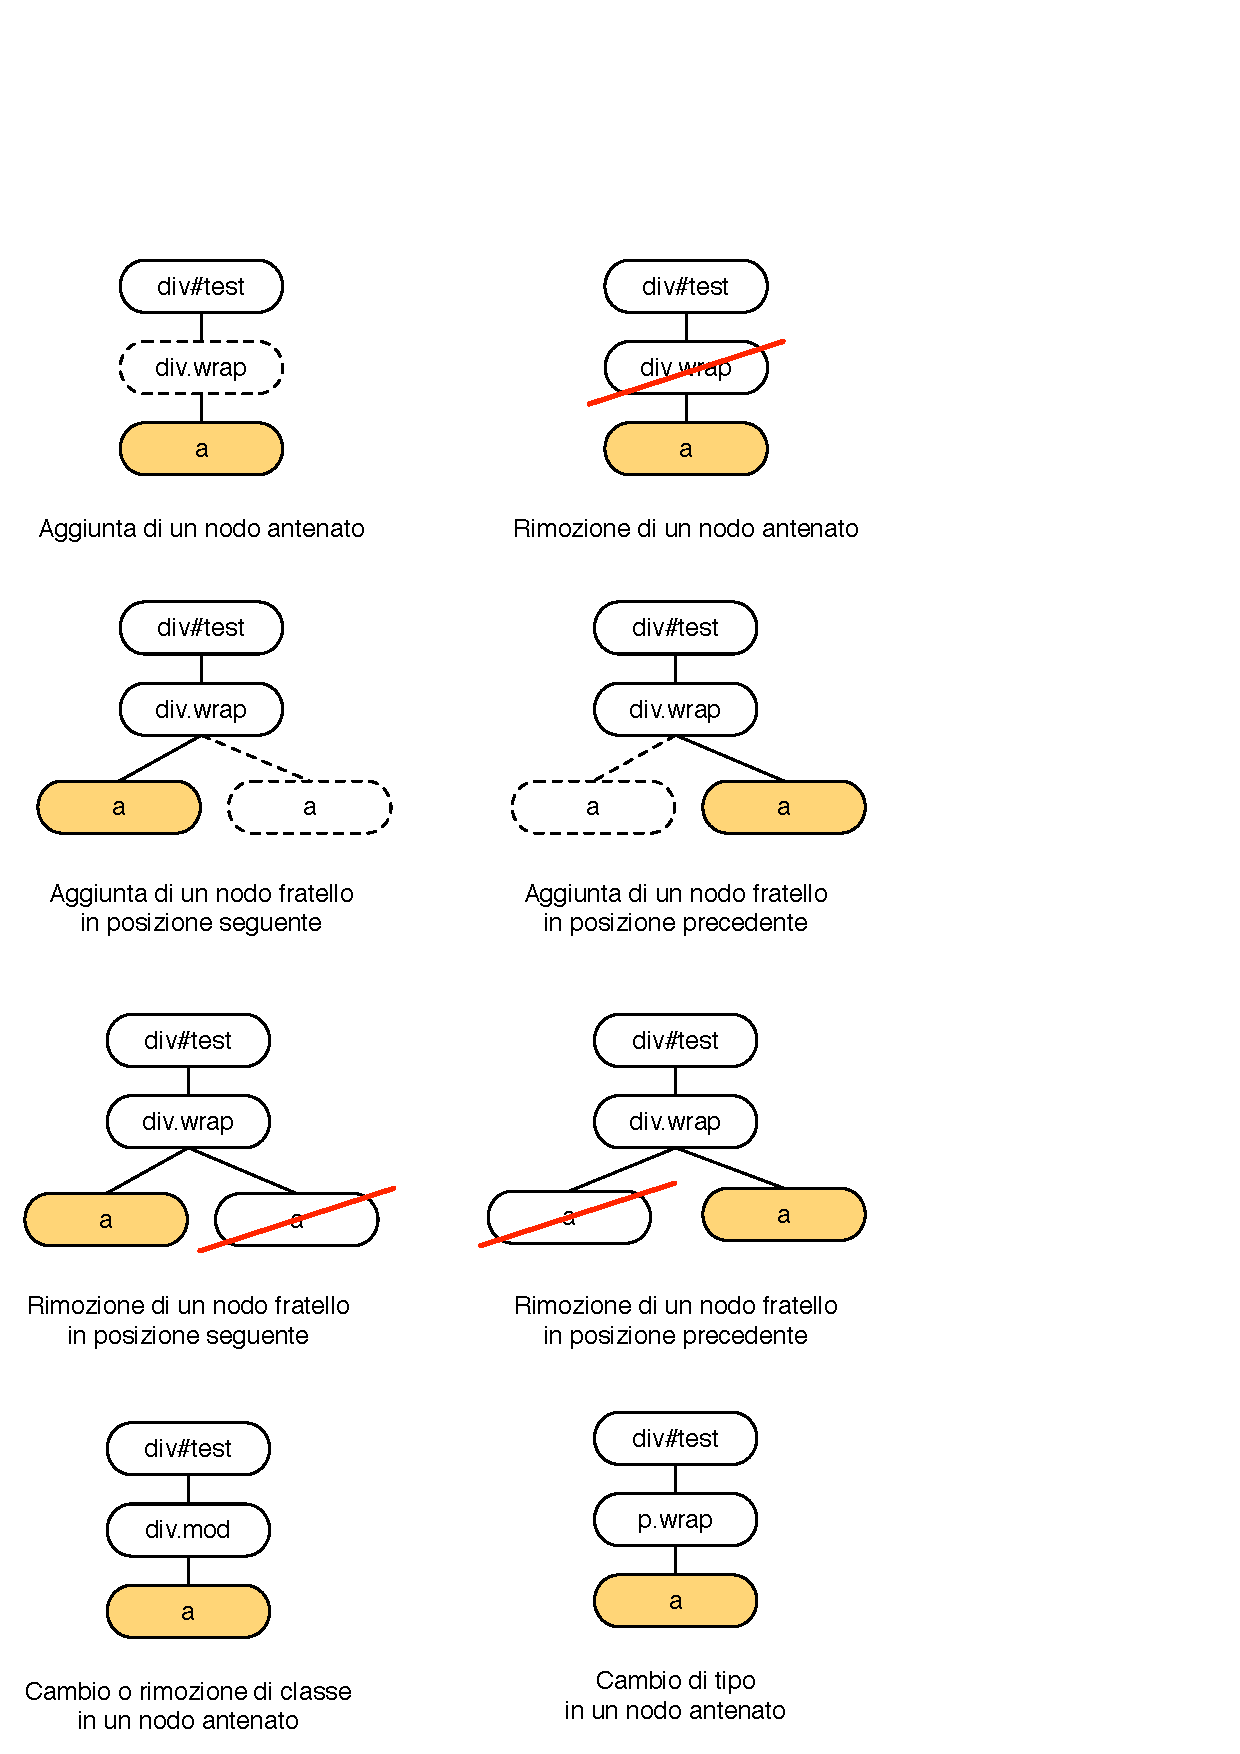
\includegraphics{images/dom_mod.png}
\caption{Principali schemi di modifica del DOM}
\label{fig:domMod}
\end{center}
\end{figure}

\subsection {L'importanza dell'attributo id}

L'algoritmo proposto attribuisce una notevole importanza all'attributo id assegnabile ai tag HTML. Secondo la specifica W3C, l'attributo id deve essere utilizzato come identificatore univoco per un elemento della pagina. Di conseguenza, se in fase di scrittura dell'HTML si sceglie di assegnare questo attributo ad un tag, si può dedurre che esso agli occhi dello sviluppatore svolge un ruolo ben preciso ed ha pertanto la sua importanza nella pagina. Essendo univocamente identificato inoltre sarà sempre possibile accedere a tale elemento indipendentemente dal contesto in cui esso si trova. 

Inoltre, questo identificativo rappresenta il modo più performante e sicuro per accedere all'elemento da codice Javascript, tramite il metodo \verb|document.getElementById|. Siccome spesso l'id viene assegnato proprio con questo scopo, è relativamente poco probabile che esso venga modificato o rimosso in un secondo momento rispetto ad altri attributi, poiché ciò comporterebbe anche la potenziale modifica degli script sviluppati per l'applicazione.

Idealmente, se tutti gli elementi del DOM avessero un attributo id il problema che l'algoritmo tenta di risolvere sarebbe inesistente, poiché la selezione del nodo di interesse non dovrebbe tener conto della posizione nell'albero. Questa osservazione giustifica di fatto il peso che l'algoritmo gli assegna. 

Più l'albero del DOM è complesso, più alta è la probabilità che si verifichi prima o poi una variazione che interessi indirettamente il percorso verso il nodo di interesse. L'algoritmo cerca pertanto di semplificare le condizioni di partenza lavorando su di un sottoalbero che contiene il nodo da selezionare. Come radice di questo sottoalbero viene scelto il primo nodo antenato che possiede un attributo id, incontrato visitando in maniera bottom-up la gerarchia del nodo da selezionare. 

Nel caso banale in cui il nodo da selezionare possieda egli stesso un id, il sottoalbero coinciderà con esso. Negli altri casi invece si avrà come punto di partenza del selettore un nodo con attributo id, che quindi avrà le proprietà descritte poco prima, limitando quindi le potenziali combinazioni di variazioni relativamente alla struttura dell'intero documento. Per costruzione il selettore CSS risultante avrà in prima posizione un frammento di tipo id, che sarà anche l'unico presente, nel caso in cui nodo abbia almeno un elemento antenato con questo attributo impostato. 

\begin{figure}[htbp]
\begin{center}
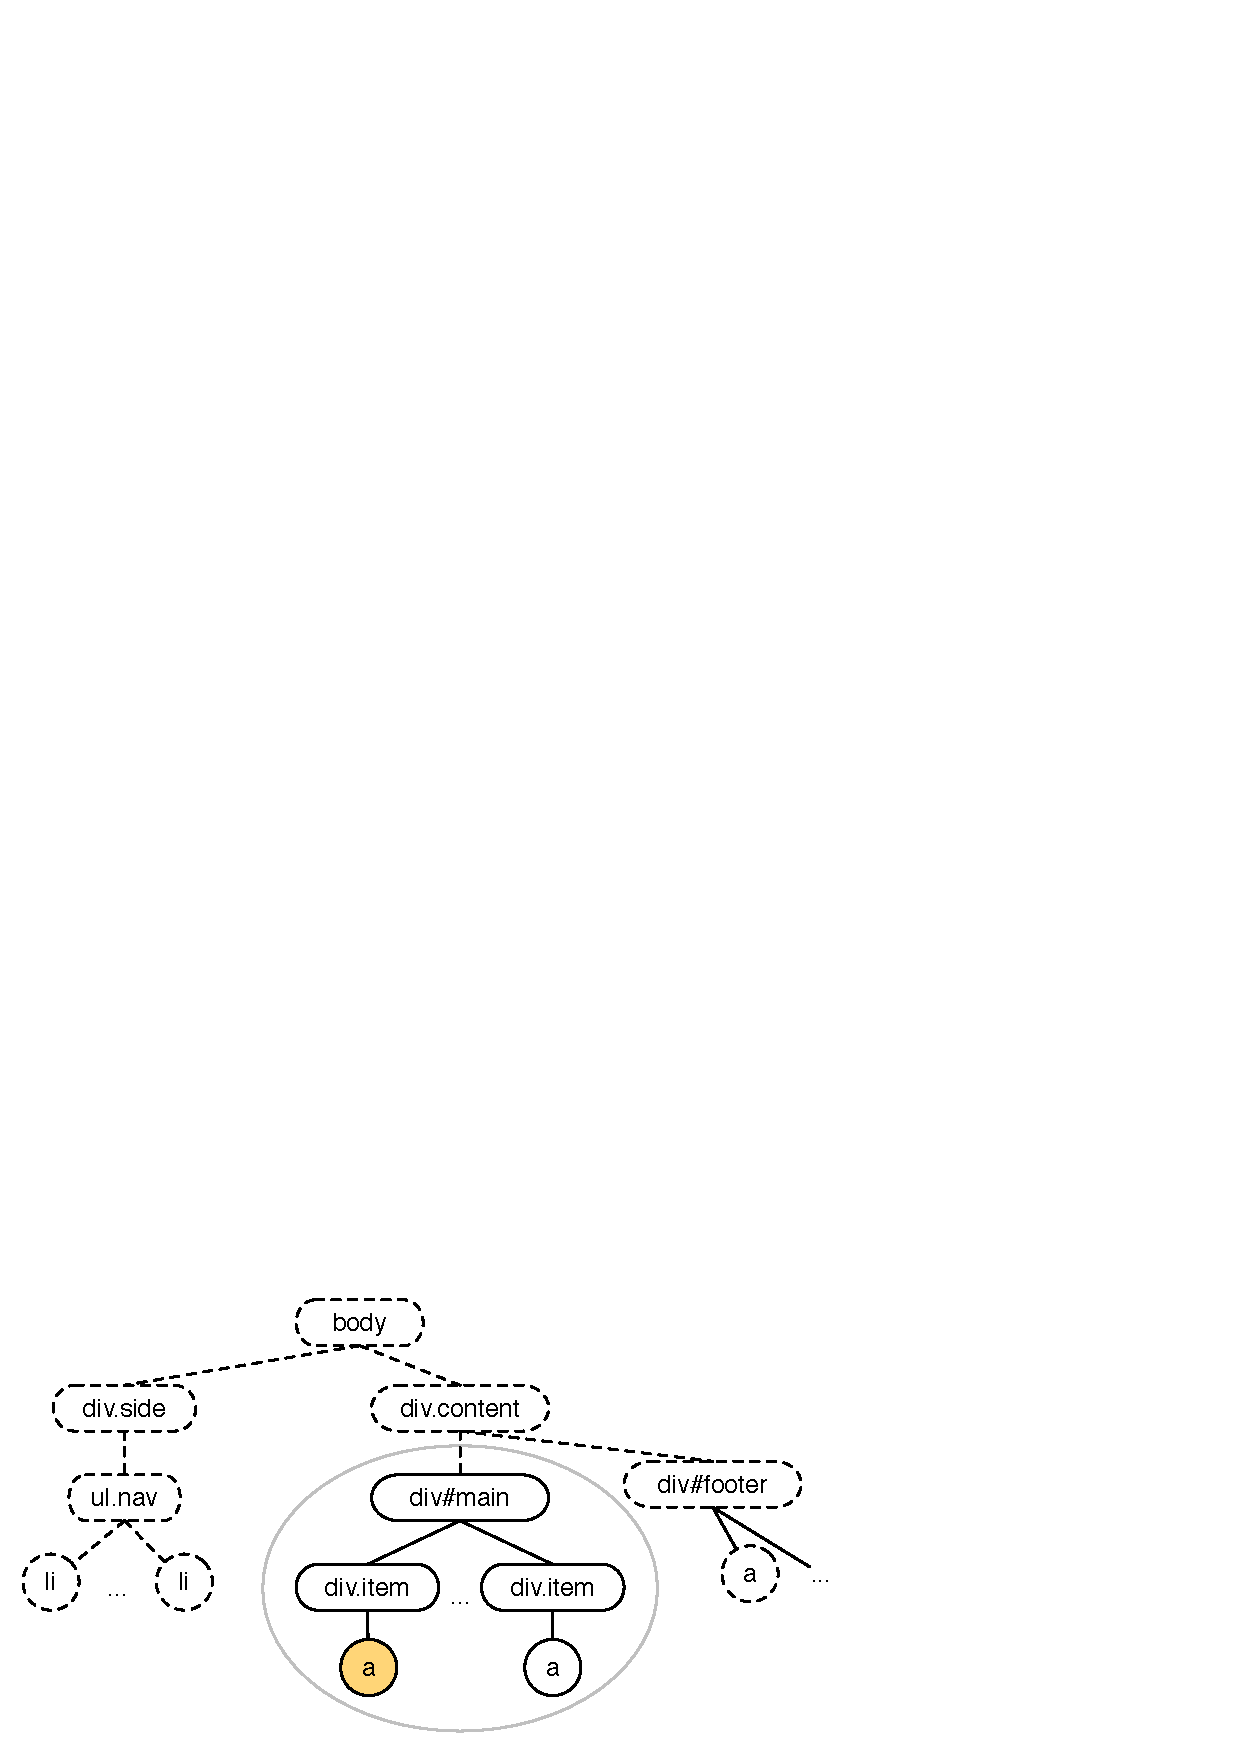
\includegraphics{images/id_partition.png}
\caption{Identificazione del sottoalbero a partire dall'ID}
\label{fig:idPartition}
\end{center}
\end{figure}

Il problema di selezionare in modo flessibile i vari componenti in fase di testing è una problematica che come si è detto interessa anche le applicazioni tradizionali con interfaccia grafica. In questo ambito una delle soluzioni spesso utilizzate comporta l'utilizzo di una o più classi ausiliarie che svolgono il ruolo di repository per i componenti. Tramite queste classi è possibile accedere in maniera opaca ai vari widget durante i test, poiché esse implementano al loro interno la logica per individuare il componente, mappandone la reale posizione ad un identificativo. Quando viene modificata la struttura dell'interfaccia, è quindi sufficiente modificare il codice in un solo punto, senza modificare l'implementazione dei test.

Nel caso delle applicazioni web con interfaccia in HTML, l'attributo può svolgere concettualmente lo stesso ruolo dell'identificativo nel repository dei widget, con il vantaggio che questa possibilità è intrinseca alla tecnologia utilizzata.

Durante lo sviluppo dell'interfaccia è buona norma quindi procedere con un occhio di riguardo per la successiva fase di acceptance testing e adoperare gli accorgimenti necessari per renderla più facile. Per quanto visto fino ad ora, può essere molto utile assegnare gli attributi id agli elementi più importanti della pagina, che permettono all'utente di attivare le funzionalità principali oppure che forniscono le informazioni di maggiore interesse, e tenere il più possibile costanti i valori di questi identificativi durante le successive modifiche, in modo da non influenzare i test definiti.

\subsection {L'attributo role}

Un altro importante attributo utilizzato dall'algoritmo è l'attributo \verb|role|. Se presente, esso serve ad indicare uno o più ruoli che l'elemento possiede nell'ambito della pagina. Un corretto uso semantico di questo attributo viene illustrato nella specifica del W3C [\url{http://www.w3.org/TR/xhtml-role/#s_role_module_attributes}]:

\lstinputlisting[language=Html, caption={Esempio di uso semantico dell'attributo role}, label=code:roleAttr]{code/selector/w3c_role.html}

Se chi ha scritto il codice HTML ha inserito questo attributo in un tag, con molta probabilità il suo valore può essere un buon candidato per selezionare l'elemento stesso in mancanza di un attributo id, oppure per costruire il percorso verso l'elemento da selezionare se l'attributo si trova su di un elemento antenato. 

In quest'ultimo caso l'attributo può aiutare ad identificare il sottoalbero in cui si trova l'elemento di interesse, corrispondente ad un'area nella pagina web.

\subsection {Selettori per elementi particolari}

In base al tipo e valore semantico dell'elemento da selezionare, l'algoritmo adopera una strategia particolare per un sottoinsieme di elementi DOM che hanno attributi particolari:

\begin{description}
\item[Campi di input] Alcuni tipi di tag HTML sono definiti per permettere all'utente di inserire dei dati in ingresso, processabili poi lato server. La loro strategia di selezione è pertanto fondamentale in fase di testing. Per questi elementi di input, come caselle di testo, caselle di spunta, menù a tendina, è di particolare interesse l'attributo \verb|name|. 

Il valore assegnato a tale attributo viene utilizzato nell'invio della richiesta HTTP successiva alla sottomissione del form come chiave che identifica il dato inserito dall'utente nel relativo campo. Lato server l'applicazione utilizza quindi il valore dell'attributo \verb|name| per accedere al dato inviato. Siccome esiste questa dipendenza all'interno dell'applicazione, è poco probabile che l'attributo name venga modificato in seguito a modifiche grafiche nel layout della pagina.Per questo motivo, è un ottimo candidato per identificare in maniera consistente e robusta il nodo del DOM in mancanza dell'attributo id.

\item[Label] Il tag \verb|label| è stato definito appositamente per comunicare all'utente il tipo di dato a inserire in un campo di testo. L'algoritmo ne utilizza l'alttributo \verb|for|, che se presente specifica l'id del campo di input a cui si riferisce il testo dell'etichetta. Per gli stessi motivi indicati nel punto precedente è possibile sfruttare questa informazione aggiuntiva nel selettore generato.

\item[Liste] Per definire liste ordinate di elementi in una pagina in maniera semantica si utilizza l'apposito tag \verb|ol|. Nel selettore CSS che individua un particolare elemento di questo tipo di liste l'algoritmo ne specifica sempre l'ordine, utilizzando lo pseudo selettore \verb|:eq(n)| messo a disposizione dalla libreria jQuery, che estende le capacità dei selettori CSS con alcuni pseudo-selettori aggiuntivi.

\item[Collegamenti ipertestuali] Anche i collegamenti ipertestuali giocano un ruolo centrale durante la fase di testing. Nel caso in cui non siano definiti attributi di tipo id o class, l'algoritmo utilizza lo pseudo selettore \verb|:contains()| di jQuery, che seleziona un elemento in base al testo contenuto.

Le alternative analizzate per questo particolare caso sono state la selezione in base alla posizione rispetto al nodo padre oppure in base all'url specificato nell'attributo \verb|href|. Entrambe queste alternative si sono però rivelate meno efficaci. La posizione è infatti una variabile poco significativa, che rende la selezione troppo fragile alle modifiche. Il valore dell'alttributo \verb|href| invece è stato scartato poiché l'url di un link è eccessivamente soggetto a modifiche interne all'applicazione, anche di piccola entità come l'aggiunta di un parametro alla querystring o casistiche simili.

\end{description}

\subsection {Descrizione dell'algoritmo}

All'interno dell'applicazione sviluppata, si è implementato l'algoritmo proposto utilizzando il linguaggio Javascript e la libreria jQuery. Quest'ultima è stata impiegata in questo ambito per due motivi. In primo luogo, jQuery fornisce dei metodi di navigazione dell'albero DOM molto potenti e di comodo utilizzo, senza bisogno di dover ricorrere all'API di Javascript per reimplementare queste funzionalità. In secondo luogo, jQuery estende le capacità dei selettori CSS3 con nuovi pseudo-selettori, che in alcuni casi rappresentano una scorciatoia per selettori più complessi usati frequentemente, mentre in altri casi esprimono concetti non definibili tramite i selettori standard. In aggiunta, è possibile ampliare questo insieme di pseudo-selettori realizzandone di personalizzati se necessario.

Il funzionamento dell'algoritmo per la generazione dei selettori CSS è diviso in due fasi distinte. 

Nella prima fase si costruisce in maniera ricorsiva il selettore, partendo dal nodo di interesse e visitando l'albero in maniera bottom-up. Durante questo processo sono tenuti in considerazione i criteri esposti in precedenza per comporre le singole parti del selettore, basandosi sull'elemento corrente in ogni iterazione.

Nella seconda fase il selettore così ottenuto viene ottimizzato dal punto di vista delle potenziali variazioni future subite dall'albero del DOM, in seguito a modifiche grafiche o di contenuto dell'applicazione sotto esame. Procedendo per tentativi l'algoritmo tenta di eliminare le componenti non indispensabili, per ottenere un selettore minimo.

Queste due fasi vengono descritte nel dettaglio nei paragrafi seguenti.

\subsubsection {Prima fase: percorso bottom-up}

La prima fase viene realizzata attraverso la funzione \verb|_traverse|. Come parametro in ingresso l'algoritmo si aspetta un riferimento ad un oggetto Javascript che rappresenta il nodo del DOM da selezionare. I passaggi dell'algoritmo sono i seguenti:

\begin{enumerate}
\item Se l'elemento corrente è il tag \verb|body|, la ricorsione viene terminata e si restituisce il selettore generato fin'ora, poiché si è raggiunta la radice dell'albero.
\item Viene prodotto il componente del selettore che specifica l'elemento corrente:
	\begin{enumerate}
		\item Se per l'elemento corrente è stato definito l'attributo id, questo viene aggiunto  in fronte al selettore costruito fino ad ora.
		\item Se l'elemento è di tipo \verb|a|, viene preposto il frammento \verb|a:icontains(<contenuto del tag>)|, che seleziona il nodo che contiene il testo specificato nelle parentesi dello pseudo-selettore jQuery.
		\item Se l'elemento possiede uno o più attributi \verb|role|, viene aggiunto un frammento del tipo \verb|<tipotag>[role=<role>]|.
		\item Se l'elemento è un widget di input e possiede l'attributo \verb|name|, si aggiunge un frammento del tipo \verb|<tipotag>[name=<name>]|
		\item Se l'elemento è una label è presente l'attributo \verb|for| e nella pagina esiste un nodo con attributo id uguale al valore dell'attributo for, si aggiunge un frammento del tipo \verb|<tipotag>[for=<for>]| 
		\item Se l'elemento è una voce di un elenco numerato, viene specificato il numero ordinale che ne indica la posizione tra i figli del nodo \verb|ol| genitore, tramite lo pseudo-selettore \verb|:eq(<indice>)|
		\item Se l'elemento possiede una o più classi, viene presa la prima in ordine di definizione e aggiunto in cima allo stack un componente al selettore del tipo \verb|.<classe>|
		\item Infine, se nessuna delle condizioni precedenti è applicabile, si aggiunge al selettore il nome del tag corrente.
	\end{enumerate}
\item Si verifica se il selettore costruito fino a questo punto identifica uno ed un solo elemento tra tutti i figli del genitore del nodo corrente.
	\begin{enumerate}
		\item Se la verifica ha esito positivo, il selettore generato fino a questo punto è univoco. Si continua la ricorsione richiamando il metodo \verb|_traverse| passandogli come argomenti il padre dell'elemento attuale, che diventerà l'elemento corrente della prossima iterazione, e il vettore contenente le componenti del selettore generate.
		\item In caso contrario, esistono almeno due nodi nella partizione dell'albero visitata che rispondono allo stesso selettore. Siccome questo sarà sempre vero anche per le iterazioni successive, è necessario rimediare al problema. Per far ciò, si ricava l'indice posizionale dell'elemento identificato dal selettore in cima allo stack dei frammenti, relativamente al nodo genitore. Si appende poi a tale frammento lo pseudo-selettore \verb|:eq(<indice>)|. Poiché questa operazione viene effettuata ad ogni iterazione dell'algoritmo, si ha la certezza che il selettore così ottenuto sia univoco per costruzione, poiché l'indice posizionale è l'elemento sicuramente discriminante in caso di ambiguità.
	\end{enumerate}	
	
\end{enumerate}

Al termine di questo procedimento si ottiene quindi un selettore univoco per l'elemento iniziale, composto da un frammento per ogni livello del DOM incontrato nella visita.

\subsubsection {Seconda fase: ottimizzazione del selettore}

Il selettore ottenuto tramite la fase precedente viene semplificato per ottenere un nuovo selettore che identifichi lo stesso elemento di partenza, ma che sia più resistente alle potenziali modifiche apportate alla struttura della pagina.

La fase di ottimizzazione si basa sulla seguente ipotesi, ricavata in maniera empirica durante lo sviluppo delle interfacce di numerose applicazioni web, che si basa sull'osservazione del punto dell'albero DOM in cui avvengono le modifiche durante lo sviluppo dell'interfaccia nel lungo periodo. Considerando come punto di riferimento la posizione nel DOM del nodo selezionato per il test, è più probabile che le modifiche si verifichino nei livelli gerarchici più vicini al punto di riferimento, piuttosto che nei livelli più distanti. Si identifica quindi una certa località nella distribuzione delle modifiche rispetto al nodo di interesse.

Questa ipotesi si fonda sul fatto che la struttura di una pagina web segue normalmente uno schema comune, nella quale gli elementi più in alto nel DOM sono utilizzati per definire la struttura di base del layout grafico, come l'intestazione della pagina, l'area dei contenuti principali, la barra di navigazione laterale, eccetera. E' ragionevole supporre che, una volta definite, queste macro aree rimarranno stabili e non subiranno modifiche continue durante lo sviluppo incrementale dell'interfaccia.

Viceversa, saranno gli elementi più interni a subire il maggior numero di modifiche, con l'aggiunta di nuovo contenuto, nuove voci nei menù, e la riorganizzazione delle strutture interne.

Sfruttando queste considerazioni, l'algoritmo prova a rimuovere progressivamente i frammenti del selettore, partendo dal frammento subito precedente a quello riferito al nodo di interesse, che rimane pertanto sempre presente. Se il selettore ottenuto continua ad identificare univocamente lo stesso elemento di partenza, il frammento corrente viene rimosso e si procede con quello che lo precede. Il procedimento viene interrotto quando si raggiunge il primo frammento di tipo id.

Di seguito vengono esposti nel dettaglio i vari passaggi di questa fase:

\begin{enumerate}
\item Si marca il nodo di partenza aggiungendovi una classe speciale, per poter verificare successivamente se il selettore ottimizzato continua ad identificare effettivamente lo stesso elemento.
\item Il vettore \verb|path| è popolato con i frammenti del selettore ottenuto dalla prima fase. In prima posizione è presente il frammento più generico, in ultima quello relativo al nodo di partenza.   
\item Per ogni elemento del vettore \verb|path|, partendo dal penultimo e procedendo con indice decrescente:
	\begin{enumerate}
		\item Se il frammento corrente è di tipo id, si interrompe l'iterazione e si ritorna il selettore corrente
		\item In caso contrario, si duplica il vettore, si rimuove dalla copia il frammento corrente e si compone il nuovo selettore unendo gli elementi del vettore di prova.
		\item Si recupera l'insieme dei nodi del DOM che rispondono a tale selettore di prova e si verifica che esso sia composto da un unico elemento. Inoltre, questo elemento deve possedere la classe speciale usata come marcatore, per assicurarsi che il selettore identifichi esattamente il nodo di partenza.
		\item Se queste condizioni sono verificate, il vettore di prova diventa il vettore del selettore corrente. L'algoritmo procede e l'analisi si sposta sul frammento precedente.
	\end{enumerate}
\end{enumerate}


\end{document}

